\chapter{引言}
\label{ch:introduction}

\section{研究背景与问题提出}

在我国加快推进数字中国建设与 “双碳” 目标实现的宏观背景下，数字经济正在成为重塑经济结构、推动能源体系转型的核心力量。数字技术通过数据要素的高效配置、产业模式的创新升级以及绿色技术的广泛渗透，深刻影响能源生产、传输、消费与管理方式，为能源结构低碳化转型提供了重要动力。国家数据局发布的《“数据要素 × 绿色低碳” 三年行动计划研究报告》进一步明确，数据要素与数字技术将深度赋能能源效率提升、碳排放管控与新型电力系统建设，为区域能源转型提供制度与技术双重支撑\cite{guojia2025}。当前关于省域数字经济与能源结构关系的研究已积累较为丰富的成果，相关研究普遍采用面板数据与空间计量方法检验数字经济对能源消费、碳排放及能源结构转型的影响，但多数研究仍依赖传统统计分析、计量模型与二维图表进行结果呈现，难以直观展现数据的时空分布特征，也无法支持灵活的交互查询与沉浸式理解。

增强现实技术凭借虚实融合、空间定位、三维可视化和自然交互等优势，能够将抽象的经济能源数据转化为直观可视、可漫游、可对比的沉浸式场景。增强现实（Augmented Reality，AR）与空间地理信息的融合应用已在智慧城市、环境监测等领域展现出显著优势，空间定位与虚实注册技术的持续进步为复杂数据场景化呈现提供了可靠支撑\cite{Liu_Jia_Nie_Rosenberg_Interrante_Zhu-Tian_2025}\cite{esri2026}。然而，将数字经济与能源结构的实证研究同多模态自然交互（手势、射线、语音与大语言模型）、沉浸式可视化以及大模型智能交互相结合的系统性成果仍然较为缺乏，相关理论框架、系统设计与应用验证均有待完善。基于这一现实背景，本文开展省域数字经济与能源结构的 AR 沉浸式分析系统研究，旨在构建集数据测算、实证分析、三维呈现与智能交互于一体的综合分析框架，为区域能源转型与数字经济融合发展提供新的研究范式与决策工具。


\section{研究意义}

本文的研究意义主要体现在理论与实践两个层面。在理论层面，本研究有助于丰富数字经济驱动能源结构转型的理论体系，完善多学科交叉的分析框架，同时拓展增强现实技术在经济管理与能源政策领域的应用边界，推动区域经济研究从传统静态展示向沉浸式、交互化、智能化方向升级。在实践层面，构建的 AR 沉浸式分析系统能够为政府部门提供直观、动态、可比较的决策支持工具，帮助决策者快速把握省域数字经济与能源结构的时空差异与演变趋势，提高政策制定的精准性与时效性。同时，该系统也可为科研教学、成果展示与公众科普提供沉浸式平台，降低复杂经济能源数据的理解门槛，推动研究成果更高效地服务于社会需求。


\section{国内外研究现状}

在数字经济与能源结构研究领域，国内外学者围绕数字经济的内涵测度、能源结构转型影响因素以及二者之间的作用机制开展了大量研究。已有研究普遍证实，数字经济能够通过提升资源配置效率、推动技术创新、促进产业结构升级等路径降低能源消耗、推动清洁能源替代并改善碳排放水平。相关研究多采用面板数据模型、空间计量模型与中介效应模型开展实证检验，部分研究从绿色金融、产业结构调整等视角揭示了数字经济影响碳减排与能源转型的中间机制，但研究成果的呈现方式仍以传统图表为主，在时空信息表达与交互体验方面存在明显局限。\cite{fu2025}\cite{shihongyuan2026}

在 AR 可视化与空间交互领域，视觉 SLAM（Simultaneous Localization and Mapping，同时定位与建图）、视觉惯性融合定位、三维渲染以及虚实融合注册技术日趋成熟，相关应用已广泛覆盖地理信息、智慧城市、工业运维、教育培训等场景。在 AR 手势交互方面，深度骨骼关键点检测与手势分类方法的进展\cite{wang2026ar_io_survey}\cite{sun2024ar_gesture_survey}为穿戴式空间交互提供了稳健的输入基础；沉浸式可视化方面，空间数据叙事与多视图联动技术\cite{Liu_Jia_Nie_Rosenberg_Interrante_Zhu-Tian_2025}\cite{chen2025immersive_econ}在经济地理场景中逐步受到关注。AR 在空间数据理解与决策支持方面的优势得到大量实证研究验证，混合现实设备的空间建模与实时跟踪能力不断提升，为多维度数据的沉浸式呈现提供了技术保障。\cite{panzeri2026cartographic}\cite{siriborvornratanakul2024ar_vr_review}尽管 AR 在空间数据可视化方面具备天然优势，但面向省域尺度经济能源面板数据的沉浸式分析系统仍然较少，尤其缺乏针对计量分析结果的定制化呈现方案。

在大模型与 AR 融合方面，最新研究表明，大语言模型（Large Language Model，LLM）能够显著增强 AR 系统的自然语言理解、空间推理、知识问答与场景生成能力，使得沉浸式交互更加智能与流畅。大模型与扩展现实的结合已形成较为清晰的技术范式，在场景理解、语音驱动交互与空间智能体等方向快速突破\cite{wang2026ar_io_survey}\cite{lee2024gazepointar}\cite{li2025llm_ar_fusion}。然而，现有融合应用多集中于通用场景，与能源经济机制、实证模型结论以及区域政策分析的结合仍较为薄弱，难以直接支撑专业化决策分析。

综合来看，现有文献在数字经济与能源结构的理论机制、实证方法以及 AR 技术应用等方面均取得了重要进展，但仍存在三方面明显不足，且这些不足与本文的研究动机直接对应。首先，传统研究呈现方式以静态二维图表为主，难以直观反映省域数据的时空异质性与区域差异，交互性与可读性较弱，这直接限制了实证结论向决策场景的高效传递——本文由此将 AR 沉浸式可视化作为核心呈现手段（对应第\ref{ch:ar_visualization}章）。其次，AR 系统在经济能源领域的应用缺乏针对性，穿戴场景下的传统键鼠交互可达性差、指令易误触，未能与实证分析框架深度结合——本文由此将多模态自然交互引入经济能源分析任务（对应第\ref{ch:ar_interaction}章）。最后，大模型与 AR 的融合尚未充分服务于能源经济机制解释、政策推演与智能问答等核心需求，且存在幻觉风险与计量结论混用的隐患——本文由此将 LLM 限定为受约束的纠错与解释层（对应第\ref{ch:ar_interaction}章第\ref{sec:ch3_speech_llm}节）。基于上述研究缺口，本文以构建一体化 AR 沉浸式分析系统为切入点，将数字经济与能源结构的实证分析同三维可视化、多模态交互（手势、射线、语音与大语言模型）与智能分析相结合，形成从理论、数据、系统到应用的完整研究链条。

为增强“现有不足—本文动机—研究内容”的可核对对应关系，表\ref{tab:gap_motivation_map}将主要不足与本文对应章节及预期作用加以对齐，便于读者把握全文的逻辑闭环。

\begin{center}
    \captionof{table}{\label{tab:gap_motivation_map}研究缺口与本文对策及章节对应}
    \small
    \begin{tabular}{p{3.6cm}p{4.6cm}p{3.8cm}p{3.2cm}}
    \hline
    研究缺口 & 本文动机与切入点 & 主要研究内容承载 & 预期作用 \\
    \hline
    传统二维呈现难以连续阅读省域时空证据链 & 以 AR 将地图、时序与计量面板绑定在同一视野与同一状态语义下 & 第\ref{sec:ch4_req}节—第\ref{sec:ch4_summary}节可视化与状态驱动联动 & 降低“图—表—文”切换成本，提升证据一致性 \\
    穿戴场景下键鼠交互可达性差、指令易误触 & 引入手势、射线、语音等多模态互补，并做稳定化与冲突消解 & 第\ref{sec:ch3_arch_overview}节—第\ref{sec:ch3_fusion}节多模态交互与融合 & 提升走动式讲解与临场操作可行性 \\
    大模型易与计量结论混用、存在幻觉风险 & 将 LLM 限定为纠错/解释层，并与数据引擎解耦 & 第\ref{sec:ch3_speech_llm}节及第\ref{sec:ch4_arch}节数据流设计 & 在增强自然语言交互的同时维持可审计性 \\
    实证结论与展示口径易脱节 & 以统一变量口径导出数据资产并驱动可视化 & 第\ref{ch:empirical_de_es}章与第\ref{sec:ch5_viz}节沉浸阅读链路 & 支撑“统计结果可沉浸核对” \\
    \hline
    \end{tabular}
\end{center}

\section{技术路线与创新点}

本文综合运用多种研究方法以保证研究的科学性与系统性。在理论分析方面，采用文献研究法梳理相关理论与研究进展，构建研究框架。在数据测度方面，采用指标综合评价法完成数字经济与能源结构指数的计算。在实证分析方面，运用面板数据模型、空间分析与相关性分析方法揭示影响效应与区域差异。在系统开发方面，采用工程化设计方法完成 AR 系统的架构、模块实现、测试与验证，并结合用户体验法评估系统有效性。整体技术路线遵循从理论到实证、从设计到实现、从分析到应用的逻辑，确保研究过程严谨且成果具备实际应用价值。

本文的创新之处主要体现在研究范式、技术融合与应用落地三个方面。在研究范式上，将传统经济能源实证研究与沉浸式 AR 可视化相结合，实现从二维结果展示向三维空间交互分析的跨越。在技术融合上，将面向省域数据场景的多模态交互（手势、射线、语音与大语言模型（Large Language Model，LLM）语义层）引入经济能源分析领域，并在几何判据手势管线基础上引入轻量神经网络分类器（DBEW-NN），以可忽略的端侧开销（1.32\,ms推理时延、221.5\,KB内存）将手势识别宏平均F1由0.700提升至0.967，提升操作效率与决策解释能力。在应用层面，构建了集实证模型、数据展示、智能问答与政策推演于一体的完整系统，可为相关领域提供可复用、可推广的决策支持工具。


\section{本文研究内容}
\label{sec:research_content}

本文围绕省域数字经济与能源结构的 AR 沉浸式分析系统展开研究，核心工作涵盖以下四个方面：

\textbf{（1）多模态交互通道构建（第\ref{ch:ar_interaction}章）。}面向 AR 穿戴场景下传统键鼠交互可达性差、指令易误触的痛点，设计并实现手势、射线、语音与大语言模型（Large Language Model，LLM）协同的多模态交互管线。在手势通道中，提出基于深度骨骼约束的边沿触发—时间窗离散化手势管线（DBEW--Gesture），通过骨骼坐标建模、几何判据分型与边沿触发—冷却窗—稳定帧三重门控，实现低误触、低连发的高频短指令交互；在此基础上引入轻量1D-CNN+Self-Attention神经网络分类器（DBEW-NN），以即插即用方式替代几何分型前端，在保持触发管线不变的前提下将手势识别宏平均F1提升至0.967。在语音通道中，构建离线自动语音识别（Automatic Speech Recognition，ASR）与受约束 LLM 增强的联合链路，通过词表约束、模板约束与拒识机制保障语音指令的准确性。在多通道协同层，提出通道内稳定化—跨通道时间窗仲裁—队列串行提交（TSTQ--Fusion）融合机制，确保手势、语音、射线事件的统一收敛与状态一致性。

\textbf{（2）AR 沉浸式可视化系统实现（第\ref{ch:ar_visualization}章）。}面向计量经济分析中"证据可核对、视图可追溯"的核心需求，设计并实现状态驱动的条件刷新多视图可视化管线（SDCR--Vis）。系统采用"交互层—数据层—查询与映射层—呈现层"四层递进架构，以统一状态向量 $\mathbf{s}_t$ 驱动省域地图、时间轴、结果面板与机制图的协同刷新。可视化编码采用归一化—通道映射—状态提交三步形式化公式，使计量结论与空间呈现同源可控。系统基于 Unity 游戏引擎与 Rokid AR Studio（Station Pro + Max Pro）实现原型部署，实测可稳定维持 30--45 FPS 的交互帧率。

\textbf{（3）省域数字经济与能源结构关系的实证分析（第\ref{ch:empirical_de_es}章）。}基于 2014--2022 年 30 省份面板数据，以熵值法与熵权—决策树融合方法构建数字经济发展水平综合指数（Digital Economy Level index，$DEL$）与能源结构优化综合指数（Energy Structure optimization index，$ES$），在面板固定效应框架下完成基准识别、非线性检验、中介路径验证与区域异质性分析，为 AR 可视化系统提供可验证的计量数据资产。

\textbf{（4）AR 沉浸式分析系统的应用验证（第\ref{ch:empirical_de_es}章第\ref{sec:ch5_viz}节）。}将第\ref{ch:ar_interaction}、\ref{ch:ar_visualization}章的系统能力与第\ref{ch:empirical_de_es}章的计量结论整合为可复现的沉浸分析会话，以任务走查方式串联"全国格局把握—计量证据核对—分区差异讨论—省域下钻阅读"完整流程，并通过小规模用户任务走查与性能监测验证系统的可用性与工程可行性。本文以 AR 系统实现为核心贡献，实证部分作为系统应用的数据基础与验证场景。

\section{论文结构}
\label{sec:paper_structure}

本文共分为六章，各章内容与逻辑关联如下：

\textbf{第\ref{ch:introduction}章 引言。}阐述研究背景、研究意义，梳理国内外研究现状，指出现有不足与本文动机的逻辑对应关系，明确研究内容、技术路线与创新点，并给出论文整体结构。

\textbf{第\ref{ch:theory}章 相关技术研究综述。}围绕AR多模态交互与沉浸式可视化两大核心技术维度，系统梳理手势识别（骨骼序列建模、轻量端侧模型、规则与学习融合）、多模态融合与冲突消解（融合分类体系、冲突类型、置信度驱动仲裁）以及AR沉浸式可视化的研究进展，明确现有工作的不足与本文的技术定位，为后续第三、四章系统设计提供直接的文献依据。

\textbf{第\ref{ch:ar_interaction}章 面向省域数据场景的 AR 多模态交互设计与实现。}作为本文的核心技术章节之一，围绕手势、语音、射线与大语言模型四大交互通道，系统阐述需求分析、架构设计、基于深度骨骼约束的手势交互算法、语音识别与 LLM 增强链路以及多模态融合与冲突消解机制。

\textbf{第\ref{ch:ar_visualization}章 状态驱动的 AR 沉浸式可视化系统设计与实现。}作为本文的另一核心技术章节，围绕计量证据的空间化呈现，系统阐述可视化系统的需求分析、四层递进架构、数据流与多视图协同机制、可视化映射方法与具体实现细节，并给出与传统桌面可视化工具的对比分析。

\textbf{第\ref{ch:empirical_de_es}章 系统应用：省域数字经济与能源结构分析。}将第\ref{ch:ar_interaction}、\ref{ch:ar_visualization}章构建的 AR 沉浸式分析系统应用于省域数字经济与能源结构关系的实证研究，完成指数构建与数据准备，并通过沉浸式 AR 会话呈现实证分析结果，验证系统在实际分析场景中的可用性。

\textbf{第\ref{ch:summary}章 总结与展望。}总结全文的学术贡献、工程创新与应用价值，指出当前研究的局限性，并对未来研究方向进行展望。

各章之间的逻辑关系为：第\ref{ch:introduction}章提出问题并明确研究框架；第\ref{ch:theory}章系统综述AR手势识别、多模态融合与沉浸式可视化的技术脉络，明确本文的技术定位与研究缺口；第\ref{ch:ar_interaction}章和第\ref{ch:ar_visualization}章是全文的核心，分别解决"如何交互"和"如何呈现"两个关键技术问题，二者共享统一状态语义并协同工作；第\ref{ch:empirical_de_es}章将前两章的技术方案应用于具体分析场景，验证系统的实际效用；第\ref{ch:summary}章对全文进行总结与展望。



\chapter{相关技术研究综述}
\label{ch:theory}

本章围绕AR多模态交互与沉浸式可视化两大核心技术维度，系统梳理手势识别、多模态融合与冲突消解、AR可视化等关键领域的研究进展与技术脉络。不同于传统学位论文将经济学理论单列一章的做法，本文将文献综述聚焦于系统实现的工程技术基础，旨在从现有工作中提炼本文方法的设计依据与创新定位，为第三章多模态交互设计与第四章AR可视化系统提供直接的技术文献支撑。

\section{AR手势识别技术综述}
\label{sec:ch2_gesture_survey}

手势识别是可穿戴增强现实人机交互的核心技术之一。本节从基于视觉与骨骼的识别方法、面向移动端的轻量模型、规则式与学习式方法的对比融合三条技术脉络梳理现有工作。

\subsection{基于视觉与骨骼的手势识别方法}

早期手势识别以RGB图像为主要输入模态，代表性工作包括基于3D卷积神经网络的动态手势在线检测与分类\cite{molchanov2016online_gesture}。该类方法直接从像素级特征学习手势的时空表示，在受控实验室条件下取得了较高精度，但对光照变化、背景复杂度和相机视角敏感，且计算开销较大，不宜直接部署于移动AR头显。

随着消费级深度相机和手部跟踪SDK的普及，\textbf{基于骨骼关键点的手势识别}逐渐成为主流范式。骨骼表示将手部姿态抽象为稀疏关节坐标集合$\mathcal{J}=\{\mathbf{p}_j\}_{j=1}^{J}$，相比稠密RGB输入具有维度低（$J\times3\ll H\times W\times3$）、视点不变性强、隐私友好等优势。Sun等\cite{sun2024ar_gesture_survey}在其综述中指出，基于骨骼关键点的深度学习方法正成为AR手势交互的主流范式——2022--2024年间发表的AR手势论文中超过60\%采用了骨骼或关键点作为输入表示。

在骨骼序列建模方面，Yan等\cite{yan2018stgcn}提出了时空图卷积网络（ST-GCN），首次将人体骨架序列统一建模为时空图结构，以图卷积同时捕获单帧内的空间关节关系与跨帧的时序动态。该工作开创了图卷积骨架动作识别方向，在NTU RGB+D数据集上大幅超越此前方法，但其约3.1M的参数量和计算开销使其不适于移动端部署。Chen等\cite{chen2021ctrgcn}进一步提出通道拓扑细化图卷积（CTR-GCN），通过学习通道特异的图拓扑，在NTU RGB+D 120上取得当时最优精度，但参数量仍较大。与图卷积路线并行发展的是基于卷积神经网络（CNN）的轻量化路线。Yang等\cite{yang2019ddnet}提出的DD-Net以手工设计的几何特征（关节对距离JCD+双尺度运动特征）替代原始坐标输入，仅用0.15M参数的1D-CNN即达到与ST-GCN可比甚至更优的精度。DD-Net的设计哲学——\textbf{几何特征先行、轻量CNN跟随}——对本文第三章DBEW--Gesture几何方法具有直接的启发意义。针对手势而非全身动作，Habib等\cite{habib2025skeleton_hgr}提出了基于数据融合与集成多流CNN的实时手势识别框架，并验证了在消费级硬件上的实时推理能力。HAN\cite{han2025hierarchical_attention}提出了一种极轻量的层次化自注意力网络，通过关节$\rightarrow$手指$\rightarrow$手掌的分层聚合，以约300倍小于GCN的计算量取得竞争性精度，再次证明了自注意力机制在骨骼手势识别中的有效性。

\subsection{面向移动端与AR边缘设备的轻量模型}

将手势识别模型部署于AR头显面临算力受限、实时性要求和功耗散热三重约束。Fertl等\cite{fertl2025hgr_edge_survey}对边缘设备手势识别的传感器技术、算法和硬件进行了全面综述，指出轻量CNN和Transformer变体是当前在精度-效率曲线上最具竞争力的架构族。Zhao等\cite{zhao2022fast_skeleton_hgr}提出了基于骨架的快速手势识别模型，将手工几何特征与自动学习的运动轨迹特征融合，以0.16M参数达到94.6\%的14类手势准确率（SHREC'17基准），展示了”几何先验+轻量学习”路线的实用性。

在模型部署方面，Zaccardi等\cite{zaccardi2023hololens_barracuda}比较了HoloLens 2上Unity Barracuda与Windows ML的ONNX推理性能，证明Barracuda在骁龙850平台上显著快于WinML，为AR头显端侧推理的工程可行性提供了实验依据。Pierdicca等\cite{pierdicca2024deepreality}开源了DeepReality框架，实现了ONNX模型经Unity Barracuda在AR Foundation中的即插即用集成。Zhang等\cite{openxr2025gesture}基于OpenXR标准的26点手部骨骼，在Meta Quest 3上以约1.3\,ms单帧推理时延达到约95\%的分类准确率，为本文DBEW-NN的轻量设计提供了直接参照。上述工作共同验证了”ONNX+Unity Barracuda”技术栈在移动XR平台上的工程可行性，本文第三章DBEW-NN的端侧部署方案（\ref{sec:ch3_nn_deployment}节）即沿袭这一范式。

\subsection{规则式方法与学习式方法的对比与融合}

在手势识别的技术谱系中，规则式方法（基于显式几何判据或有限状态机）与学习式方法（基于深度神经网络）并非互斥，而是具有互补优势。Vosinakis等\cite{vosinakis2024ar_gesture_interaction_review}对AR手势交互技术的综述指出：规则式方法在可解释性、零训练成本和确定性行为方面具有优势，但在复杂手势和新颖姿态的泛化能力上不及学习方法；学习式方法精度高、鲁棒性强，但需要标注数据与端侧推理资源。二者的典型特征对比如表\ref{tab:rule_vs_learning}所示。

\begin{center}
    \captionof{table}{\label{tab:rule_vs_learning}规则式与学习式手势识别方法的特征对比}
    \small
    \begin{tabular}{p{3.0cm}p{4.5cm}p{4.5cm}}
    \hline
    维度 & 规则式方法（几何判据） & 学习式方法（深度神经网络） \\
    \hline
    可解释性 & 高——每步判定可追溯至几何量 & 低——隐空间特征难以直接解释 \\
    训练数据需求 & 零——仅需设定阈值 & 高——需大量标注数据 \\
    参数规模 & 零——无训练参数 & 小到中——轻量模型约50--500K \\
    对新类别的扩展 & 困难——需人工分析设计规则 & 较易——重新训练/微调即可 \\
    噪声鲁棒性 & 弱——噪声直接破坏几何判据 & 强——可通过数据增强学习噪声模式 \\
    类间模糊边界 & 硬阈值导致歧义 & 软概率输出可表达不确定性 \\
    部署复杂度 & 低——常数级判断 & 中——需推理运行时+模型文件 \\
    \hline
    \end{tabular}
\end{center}

近年来，若干工作尝试融合两种范式的优势。Zhao等\cite{zhao2022fast_skeleton_hgr}将几何特征与CNN空间建模结合，属于”几何特征+轻量CNN”路线的典型代表。Yusuf等\cite{geometric_spatiotemporal_hgr2023}将几何特征提取与CNN空间建模和多头注意力时序建模结合，在DHGD和SHREC'17数据集上验证了混合方案的有效性。本文第三章的工作遵循”规则为基、学习增强、两者互补”的设计哲学：DBEW--Gesture以几何判据提供可解释的基线方法和零成本冷启动能力；DBEW-NN在保持触发管线不变的前提下以轻量NN替代几何分型前端，获得数据驱动的精度与鲁棒性提升；两者通过统一的\texttt{GestureEvent}接口共享下游触发与融合逻辑，实现了”即插即用”的工程架构。

\section{AR多模态融合与冲突消解技术综述}
\label{sec:ch2_fusion_survey}

可穿戴AR设备的多传感器配置使用户可以同时通过手势、语音和头显射线与虚拟内容交互，多通道并行输入在提升交互带宽与自然性的同时，引入了多模态冲突这一根本性挑战。本节从融合分类体系、冲突类型与消解策略、置信度的融合角色三个维度梳理现有工作。

\subsection{多模态融合的分类体系}

Heinrich等\cite{heinrich2025fusion_survey}基于PRISMA指南对50个多模态人机交互系统（2009--2025）进行了系统性分类，将融合方法划分为三大类。\textbf{早期融合}（特征级）在分类器之前合并不同模态的原始或低级特征，可捕获跨模态低层交互但面临维度爆炸——不同模态的特征维度、采样率和分布差异使得联合表示空间的设计极为复杂。\textbf{晚期融合}（决策级）对各通道独立分类后合并决策，模块化强、各通道可独立优化与回退，但无法利用跨模态低层交互。\textbf{混合融合}在子系统组内早期融合、组间晚期融合，精度最高但架构最复杂，目前主要见于研究原型。Heinrich等\cite{heinrich2025fusion_survey}指出，在50个综述系统中，晚期融合占比最高（约60\%），尤其适合传感器模态差异大的可穿戴场景。

Lu等\cite{lu2025spatial_computing}对104篇XR头显多模态交互论文（2022--2025）的综述进一步指出：手势+眼动凝视仍是最主流的多模态组合，但语音相关研究在2024年因LLM突破而激增；描述性晚期融合（规则式决策级融合）仍占主导地位，原因在于ML-based融合面临多模态训练数据稀缺的瓶颈；CARE（Complementary/Assigned/Redundant/Equivalent）模型是设计多通道分工的主要理论框架。

本文第三章TSTQ--Fusion选择描述性晚期融合+置信度驱动的动态优先级仲裁，基于以下三点考量：（1）手势（26$\times$3维骨骼坐标@60Hz）、语音（16kHz音频$\rightarrow$ASR文本，间歇触发）和射线（单次命中事件）的传感器采样率、时延特性和置信度语义各不相同，不适合早期特征级融合；（2）省域经济分析任务中跨通道冲突主要表现为相邻时刻的语义互斥输入而非严格并发，规则+置信度的组合足以覆盖多数冲突模式；（3）规则的显式性与可解释性符合计量分析对”可追溯决策”的要求。

\subsection{多模态冲突类型与消解策略}

多模态冲突是指两个或多个输入通道在同一时间窗口内发出语义互斥的指令。Wang等\cite{wang2026ar_io_survey}将冲突分为三类：\textbf{互补冲突}（两通道指令指向同一目标的不同方面，可通过合并解决）、\textbf{冗余冲突}（两通道发出语义相同的指令，可通过去重解决）和\textbf{互斥冲突}（两通道发出语义互斥的指令，需要外部仲裁机制）。其中互斥冲突是融合机制的核心处理对象。

Bai等\cite{bai2025ar_gesture_speech}对16个AR手势+语音系统的综述揭示了一个关键发现：75\%的多模态AR系统使用固定规则融合（如手势永远优先于语音），但在上下文变化时这种静态优先级策略导致错误率显著升高。Lee\cite{lee2025attentional_friction}将多模态整合不良导致的现象定义为”注意摩擦”（attentional friction），并推荐”明确反馈以降低摩擦”的设计模式——这正是本文TSTQ--Fusion中保守拒绝+AR HUD轻提示策略的理论依据。

Radlak等\cite{radlak2025probabilistic_fusion}提出了基于概率框架的多模态融合方法，通过为每个通道的每帧输出维护后验概率分布，在贝叶斯框架下联合推理最可能的事件序列。该方法在概念上与TSTQ--Fusion的置信度驱动仲裁一致，但其全事件空间推断在移动XR平台上的计算开销不可忽略。TSTQ--Fusion采用更轻量的评分函数（$O(|W_k|\log|W_k|)$复杂度）以适配骁龙XR2级别的算力预算，在最优融合精度与实时性约束之间取得工程折中。

\subsection{AR手势交互中的多模态系统集成}

将手势识别嵌入完整的AR交互系统时，需解决多通道协调问题。Wang等\cite{wang2026ar_io_survey}从输入输出双视角系统梳理了AR人机交互技术，将手势交互归为”显式控制型”输入模态，强调其在高频短指令场景下的独特价值。Shao等\cite{shao2024cv_gesture}进一步将3D手部骨骼与眼动追踪信号融合，提升了AR场景下意图理解的鲁棒性。多通道用户界面理论\cite{dong2022}为本文手势、射线、语音与大语言模型四通道的互补分工提供了理论框架。

本文第三章的多模态系统设计与上述文献形成以下对话：（1）采用CARE模型将手势定位为”显式控制通道”，与语音（符号输入）和射线（空间选择）明确分工；（2）手势事件经DBEW稳定化后以统一\texttt{GestureEvent}结构提交TSTQ--Fusion融合层，以置信度驱动动态优先级进行跨通道仲裁——直接回应了Bai等\cite{bai2025ar_gesture_speech}指出的”缺乏置信度利用”问题；（3）各通道具有独立的降级策略（如NN失败时回退至几何规则），避免了单通道故障导致系统级失效。

\section{AR沉浸式可视化技术综述}
\label{sec:ch2_vis_survey}

AR沉浸式可视化是将增强现实技术与数据分析深度融合的新型研究范式。相较于传统桌面可视化，AR可视化具有空间化、交互性、沉浸式三大核心特征：将多维度数据映射为三维空间视觉对象，支持用户通过自然交互实现数据的多维探索，并在虚实融合环境中降低复杂数据的认知门槛\cite{liu2025can}\cite{chen2025immersive_econ}。

在AR空间数据可视化方面，三维可视化理论通过数据映射与视觉编码（颜色渐变、高度映射、纹理区分等），将省域面板数据的属性与时空特征转化为直观的三维视觉元素\cite{Liu_Jia_Nie_Rosenberg_Interrante_Zhu-Tian_2025}。空间数据叙事与多视图联动技术\cite{chen2025immersive_econ}在经济地理场景中逐步受到关注，混合现实设备的空间建模与实时跟踪能力不断提升\cite{panzeri2026cartographic}\cite{siriborvornratanakul2024ar_vr_review}。在声明式图表生成方面，React框架的声明式UI范式\cite{walke2013react}对前端开发产生了革命性影响——其核心洞察”与其手动管理DOM的增量变更，不如每次声明式地描述UI应该长什么样”启发了本文第四章ChartForge将图表生成重新表述为”从意图描述到图表规约的声明式映射”。大模型与扩展现实的结合已形成较为清晰的技术范式\cite{wang2026ar_io_survey}\cite{li2025llm_ar_fusion}，在场景理解、语音驱动交互与空间智能体等方向快速突破。

然而，面向省域尺度经济能源面板数据的沉浸式分析系统仍然较少，尤其缺乏针对计量分析结果的定制化呈现方案。现有AR可视化方案在图表类型固化、需求到代码的语义鸿沟、生成质量缺乏形式化度量等方面存在局限，这构成了本文第四章ChartForge+SDCR--Vis融合架构的直接研究动机。

\section{本章小结与研究定位}
\label{sec:ch2_summary}

综合上述三个技术维度的文献综述，可提炼出以下关键研究缺口与本文的对应定位：

\textbf{在手势识别维度}，现有工作在骨骼序列建模和轻量模型部署方面取得了显著进展，但存在两方面的不足：（1）缺乏在AR经济数据分析这一特定场景下对纯几何规则与轻量NN增强两种方案的精度-效率-鲁棒性三维权衡的系统对比；（2）现有轻量模型的部署验证多集中于Meta Quest 3或HoloLens 2平台，在Rokid AR Studio（骁龙XR2+Unity Barracuda）这一国产AR平台上的端到端验证尚属空白。本文第三章以DBEW--Gesture和DBEW-NN分别覆盖两条技术路线，在同一实验框架下完成系统对比，并给出完整的ONNX$\rightarrow$Barracuda部署方案。

\textbf{在多模态融合维度}，75\%的现有AR多模态系统使用固定规则融合\cite{bai2025ar_gesture_speech}，缺乏对置信度信号的利用，且静态优先级策略在上下文变化时错误率显著升高。本文第三章TSTQ--Fusion通过置信度驱动的动态优先级仲裁（式~\ref{eq:fusion_score}）和保守拒绝机制，在规则可解释性与数据驱动适应性之间取得了工程折中。

\textbf{在AR可视化维度}，现有方案多采用固定编码图表，缺乏从自然语言意图到图表规约的声明式生成能力。本文第四章ChartForge框架将图表生成从”手写渲染代码”升级为”NL$\rightarrow$规约$\rightarrow$AR图表”的声明式AIGC范式，并保持与第三章统一状态向量的协同。

上述三个技术维度在系统层面通过统一状态向量$\mathbf{s}_t$实现闭环：手势、语音、射线经单通道处理和TSTQ--Fusion融合后更新$\mathbf{s}_t$；ChartForge+SDCR--Vis读取$\mathbf{s}_t$驱动省域地图、时间轴、图表与面板的协同刷新。这一”交互$\rightarrow$状态$\rightarrow$可视化”的架构主线贯穿本文第三、四、五章。

\chapter{面向省域数据场景的AR多模态交互设计与实现}
\label{ch:ar_interaction}

为增强方法辨识度与可引用性，本章将\textbf{深度骨骼约束下的边沿触发—时间窗离散化手势管线}简记为 \textbf{DBEW--Gesture}；将其神经网络增强版本简记为 \textbf{DBEW-NN}；将\textbf{通道内稳定化—跨通道时间窗仲裁—队列串行提交}的多模态融合机制简记为 \textbf{TSTQ--Fusion}。下文在不影响理解的前提下交替使用中文机制名与上述缩写。

\section{多模态交互架构总览}
\label{sec:ch3_arch_overview}

\subsection{任务场景与设计需求}

省域经济能源数据的沉浸式分析对交互系统提出四类核心需求。\textbf{空间选择}：用户需在三维省域Mesh上选中目标省份以驱动信息卡或筛选，头戴显示条件下传统桌面交互设备可达性差。\textbf{时序与指标控制}：需在2014--2022年时间轴上前后移动、在DEL/ES等多种指标间切换、刷新或重置视图，这些高频微调操作要求低时延、低误触。\textbf{符号信息输入}：需承载年份、地名与筛选条件等语义信息。\textbf{开放语义问答}：需对计量结果进行自然语言解释与情景推演。

依据多通道用户界面理论\cite{dong2022}，本研究采用手势、射线、语音与大语言模型（Large Language Model，LLM）四通道互补分工：\textbf{手势}侧重短促、离散而可重复的动作，适于高频微调与小集合内的模式切换（如年份步进、指标切换）；\textbf{射线}与头显前向一致，适于与省域三角网格相交完成点选、高亮与读数等空间选择；\textbf{语音}适于承载年份、地名与筛选条件等符号信息；\textbf{LLM语义层}承担纠错、归一化、问答解释与情景推演。

为明确AR手势在计量经济分析中的应用必要性，表\ref{tab:interaction_comparison}从交互可达性、空间定位精度、高频操作效率、走动场景适配性与认知负荷五个维度进行对比。

\begin{center}
    \captionof{table}{\label{tab:interaction_comparison}计量经济分析场景下不同交互方式的对比}
    \small
    \begin{tabular}{p{2.8cm}p{3.0cm}p{3.0cm}p{3.0cm}p{3.2cm}}
    \hline
    维度 & 传统键鼠 & 触屏大屏 & 纯语音 & 本文 AR 多模态 \\
    \hline
    交互可达性 & 需固定桌面，走动场景不可用 & 需靠近屏幕，视野受限 & 解放双手，但无空间参照 & 走动式自由操作，头显随身穿戴 \\
    空间定位精度 & 鼠标点击精确，但非三维 & 触屏点选直观，但限于二维平面 & 无空间定位能力，仅靠语音描述 & 射线+凝视三维空间拾取，直接命中省域 Mesh \\
    高频操作效率 & 快捷键高效，但切换窗口打断心流 & 手势操作较慢，多步菜单层级深 & 连续指令易冲突，噪声下误识率高 & 手势单帧完成年份步进/指标切换，时间窗抑制连发 \\
    走动场景适配 & 完全不可用 & 不可移动 & 移动中可用但环境噪声敏感 & 佩戴即用，支持边走边讲边指 \\
    认知负荷 & 多窗口拼接，依赖工作记忆 & 信息密度高，视线需频繁移动 & 无视觉反馈，需记忆指令集 & 空间锚定+多视图联动，同一视野场内连续阅读 \\
    \hline
    \end{tabular}
\end{center}

从控制论角度，可将交互对象抽象为有限维系统状态向量 $\mathbf{s}_t = (y_t, m_t, p_t, r_t, \ldots)$，其中 $y_t$ 为当前年份索引，$m_t$ 为当前着色指标类型，$p_t$ 为当前选中省份编码，$r_t$ 为视图刷新标记。手势、射线与浅层语音并不直接操作渲染细节，而是先改变上述离散或分段连续的状态变量，再由可视化层据状态重算映射与绘制（详见第四章SDCR--Vis管线）。LLM层可在同一状态快照之上生成解释文本与情景预测序列，但数值与回归结论须来自数据引擎，禁止模型编造。该分层使交互逻辑与数据表达解耦：同一套语义既可由骨骼手势、射线命中触发，也可由语音解析触发，从而保证多模态在状态空间上的一致性。

\subsection{系统架构设计}

架构上，系统遵循“多路输入—通道内处理—融合写状态—可视化与语义并行消费”的分层思路，如图\ref{fig:ch3_architecture}所示。

\begin{center}
  \begin{tikzpicture}[
    scale=0.88, transform shape,
    node distance=0.32cm and 0.28cm,
    box/.style={draw, rounded corners=2pt, align=center, inner sep=3pt, minimum width=2.2cm, minimum height=9mm, font=\footnotesize},
    arr/.style={-{Stealth[length=1.5mm]}, semithick}
  ]
    % Input layer
    \node[box, fill=blue!8] (gesture) {手势通道\\深度骨骼$\rightarrow$分类};
    \node[box, fill=blue!8, right=0.3cm of gesture] (ray) {射线通道\\头显位姿$\rightarrow$Mesh命中};
    \node[box, fill=blue!8, right=0.3cm of ray] (speech) {语音通道\\多麦阵列$\rightarrow$ASR};
    \node[box, fill=blue!8, right=0.3cm of speech] (llm) {LLM语义层\\纠错$\cdot$问答$\cdot$推演};
    % Channel processing
    \node[box, fill=orange!10, below=0.7cm of gesture] (gp) {手势处理\\DBEW--Gesture\\+ DBEW-NN};
    \node[box, fill=orange!10, below=0.7cm of ray] (rp) {射线处理\\碰撞检测\\+ 确认逻辑};
    \node[box, fill=orange!10, below=0.7cm of speech] (sp) {语音处理\\离线ASR\\+ LLM增强};
    \node[box, fill=orange!10, below=0.7cm of llm] (lp) {语义处理\\上下文同步\\+ 提示构建};
    % Fusion
    \node[box, fill=green!8, below=0.7cm of rp, minimum width=4.5cm] (fusion) {TSTQ--Fusion 多模态融合\\通道内稳定化$\rightarrow$跨通道仲裁$\rightarrow$队列串行提交};
    % State
    \node[box, fill=green!12, below=0.7cm of fusion, minimum width=4.5cm] (state) {统一状态向量 $\mathbf{s}_t$};
    % Output
    \node[box, fill=gray!12, below=0.7cm of state, minimum width=4.5cm] (output) {可视化刷新 + 语义输出};
    % Arrows
    \draw[arr] (gesture) -- (gp); \draw[arr] (ray) -- (rp);
    \draw[arr] (speech) -- (sp); \draw[arr] (llm) -- (lp);
    \draw[arr] (gp) -- (fusion); \draw[arr] (rp) -- (fusion);
    \draw[arr] (sp) -- (fusion); \draw[arr] (lp) -- (fusion);
    \draw[arr] (fusion) -- (state);
    \draw[arr] (state) -- (output);
  \end{tikzpicture}
  \captionof{figure}{第三章多模态交互系统总架构：四路输入经通道内处理后进入TSTQ--Fusion融合层，统一写入状态向量后驱动可视化刷新与语义输出。\label{fig:ch3_architecture}}
\end{center}

输入侧包括Rokid头戴深度流水线支撑的手部骨骼（26关节）、与头显位姿一致的前向射线及省域Mesh、以及多麦克风语音流；通道内分别完成手势分类（几何规则或NN）、射线命中检测与离线ASR—LLM口令链；融合层对离散事件仲裁后更新统一状态向量，驱动第四章所述三维地图、时间轴与面板；数据引擎为指标与回归结果提供唯一可信来源，LLM在约束提示下承担纠错、解释与归一化。

工程实现上，客户端以Unity游戏引擎与Rokid UXR组织渲染与采集，服务端以FastAPI承载LLM与数据访问，前后端经局域网以JSON进行结构化交互；手势NN模型经ONNX导出后在Unity Barracuda运行时执行推理，语音链路以Vosk离线ASR为基座辅以LLM后处理。

本章后续各节按四通道展开：手势识别领域的系统综述已前置至第\ref{ch:theory}章第\ref{sec:ch2_gesture_survey}节（AR手势识别技术综述）与第\ref{sec:ch2_fusion_survey}节（AR多模态融合技术综述），本章不再重复文献梳理，直接进入方法设计与实验评估；第\ref{sec:ch3_gesture_original}节详述原始几何判据手势交互算法（DBEW--Gesture），含数据流建模、分型规则、触发管线与用户实验；第\ref{sec:ch3_gesture_nn}节在此基础上引入轻量神经网络增强方案（DBEW-NN），按学术论文格式完整呈现数据采集、模型设计、训练策略与对比实验；第\ref{sec:ch3_bridge_gesture_fusion}节阐明从手势NN到多模态融合的置信度传递链路；第\ref{sec:ch3_speech_llm}节面向AR眼镜的特殊约束，实现离线语音识别与轻量LLM增强链路；第\ref{sec:ch3_fusion}节详述TSTQ--Fusion仲裁机制；第\ref{sec:ch3_summary}节总结全章。

\section{原始几何判据手势交互算法（DBEW--Gesture）}
\label{sec:ch3_gesture_original}

为与第\ref{sec:ch3_gesture_nn}节的神经网络增强方案相区分，本节聚焦于基于显式几何判据的规则式手势识别管线。该方案的优势在于可解释性强、无需训练数据和零参数量，适合作为基线方法。

如图\ref{tab:rokid_ges}所示，Rokid UXR2.0 SDK提供了一些基础的手势操控。但是在本文所使用的场景中基础手势无法满足多模态交互的需求。因此需要引入基于深度骨骼约束的自定义手势交互算法。
\begin{center}
  
\includegraphics[width=0.7\textwidth,keepaspectratio]{rokid_ges.png}
  \captionof{table}{\label{tab:rokid_ges}图中一共5中手势，分别为OpenPinch、Pinch、近场单指、Palm、Grip}
\end{center}

表 \ref{tab:ges_map} 给出了主要自定义手势与语义的对应关系；图\ref{fig:ar_ges_test} 展示了Rokid AR 实机手势测试的截图。
\begin{center}
    \captionof{table}{\label{tab:ges_map}自定义手势与语义对应关系表}
    \begin{tabular}{ll}
    \hline
    手势 & 语义 \\
    \hline
    单指向左 / 单指向右 & 将当前年份索引减一 / 加一 \\
    二指手心/背 &  DEL/ES 热力指标切换 \\
    三指手心/背 & 开关计量分析面板 \\
    四指手心 & 跳转至Main场景（中国地图）\\
    四指手背 & 跳转至Province场景（省级地图）\\
    握拳 & 复位 \\
    \hline
    \end{tabular}
\end{center}
\begin{center}
  
\includegraphics[width=0.5\textwidth,keepaspectratio]{arges1.png}
  \hfill
  
\includegraphics[width=0.5\textwidth,keepaspectratio]{arges2.png}
  \captionof{figure}{\label{fig:ar_ges_test}Rokid AR 实机手势测试}
\end{center}

本节将手势交互包装为可复现的算法流程，构建“基于深度骨骼约束”的手势识别与命令触发机制。算法输入为每帧手部骨骼点集 $\mathcal{J}_h^{(t)}$，经坐标统一、几何特征提取与分层分型得到手势类别 $g^{(t)}$，再通过边沿触发与时间窗抑制生成离散控制事件，最终映射到年份步进、指标切换、视图刷新等系统状态更新。该算法与射线空间选择、语音指令形成互补，目标是在 AR 场景中兼顾交互自然性、稳定性与可解释性。

在面向省域计量可视化的高频短指令场景，手势通道遵循如下原则：（1）状态优先。手势不直接操作渲染细节，只提交与第三章、第四章一致的状态增量（年份、指标、省域、刷新等），保证与数据引擎及回归面板同源；（2）低误触优先。以边沿触发、最小稳定帧与时间窗抑制抑制连发与抖动，在可穿戴噪声环境下宁可略增时延也不放大误命令；（3）单手为主、双手低频。默认单手完成步进与切换，双手组合仅保留急停等少数高代价语义，降低组合爆炸与遮挡下的识别不确定性；（4）可发现性与可替代性。同一语义允许多类手势映射（见表\ref{tab:ges_map}），兼顾遮挡与疲劳时的同义操作；（5）可解释与可审计。分型判据由几何量与阈值显式给出，便于论文复核与工程调参；（6）与平台能力对齐。关节集合、坐标系与追踪频率以设备侧手部追踪能力为上界，避免脱离 Rokid UXR 3.0可实现范围。
此外，Rokid AR 平台在 UXR 手部追踪管线中提供标准化的手部模型与关节枚举：通常将单手骨骼组织为腕、掌骨及各指节的 MCP/PIP/DIP 与指尖等层级，左右手可独立跟踪；关节位姿可在设备坐标系下输出，再经与头显位姿、外参对齐变换到世界坐标系或应用统一跟踪系，供 Unity 等客户端按帧读取\footnote{\href{https://custom.rokid.com/prod/rokid_web/c88be4bcde4c42c0b8b53409e1fa1701/pc/cn/8ad2e74dbd7c4f5bb21a964dbdd5512d.html?documentId=dbdf788eac3541a2a7d73b5e2bc1f89f}{Rokid AR 平台开发者文档（手势与手部追踪，以当前 SDK 版本为准）}}。本文所称“手势类别”并非平台内置的固定 UI 手势全集，而是在上述关节语义之上，由应用层依据几何判据（伸直数、掌心法向、食指水平投影等）自行\textbf{离散化}得到的分析用手势集合 $\mathcal{G}$；平台负责稳定输出 $\mathcal{J}_h^{(t)}$，应用负责映射 $g^{(t)}\mapsto$ 业务命令。实现时应以官方文档列出的关节索引、追踪状态标志与丢帧处理为准，在检测无效或置信度不足时丢弃该帧，避免向融合层提交空骨骼。




以下按数据流与坐标建模、几何判据与语义映射、离散命令生成依次叙述。

\subsection{数据流与坐标建模}
\label{sec:gesture_depth_skeleton}

手势输入的物理起点为头戴设备上的深度感知：深度摄像头或与 RGB 融合的深度估计流水线按帧产生场景深度图，Rokid UXR 手部跟踪在此基础上解算手部骨架各关节在传感器或相机坐标系下的三维位置，再与头显位姿、外参联合变换到统一跟踪坐标系或世界坐标系，从而得到可与虚拟省域 Mesh 直接对齐的 $\mathbf{p}_{j,h}^{(t)}$。相较于仅依赖二维图像的手势分类，基于深度的骨骼三维坐标对遮挡与尺度变化更为稳健，符合 AR 中“手—物共空间”交互对度量一致的要求\cite{wang2026ar_io_survey}。

在 Unity 运行时中，Rokid UXR 将上述手部追踪与头戴显示、空间跟踪置于同一会话：按帧回调应用逻辑，使深度估计、骨骼解算与渲染处于同一时间基准。应用层通过官方 API 读取关节枚举与坐标（关节命名、追踪状态与坐标变换以当前 SDK 及上文文档为准）。平台将单只手离散为腕、掌、各指节 MCP/PIP/DIP 及指尖等；对指定手别 $h\in\{\mathrm{L},\mathrm{R}\}$ 与关节编号 $j$，第 $t$ 帧世界系（或设备统一系）位置记为 $\mathbf{p}_{j,h}^{(t)}$，未稳定检测时须先剔除无效值。单帧关节集合记为 $\mathcal{J}_h^{(t)}=\{\mathbf{p}_{j,h}^{(t)}\}_{j\in\mathcal{K}}$。

手部与虚拟场景表达在同一世界坐标系或设备跟踪坐标系中，由 SLAM/VIO 等与头显位姿对齐；主相机外参每帧更新，可用于射线与可选的相机系投影。本研究分型以世界系下指节链向量与掌心法向为主；若需与凝视或 UI 严格对齐，可再经相机系投影判别。左右手关节集合 $\mathcal{J}_L^{(t)}$、$\mathcal{J}_R^{(t)}$ 独立处理，以降低双手组合爆炸；每帧由 $\mathcal{J}_h^{(t)}$ 提取伸直、张合、朝向等特征后进入分层判定，输出 $g^{(t)}\in\mathcal{G}\cup\{\emptyset\}$。

\subsection{几何判据、分型与语义映射}

对单指几何关系，取 MCP---PIP---DIP 相邻段单位向量 $\mathbf{e}_1,\mathbf{e}_2$，定义共线度
\begin{equation}
  c = \mathbf{e}_1\cdot \mathbf{e}_2.
  \label{eq:finger_collinearity}
\end{equation}
当 $c>\theta_{\mathrm{ext}}$（如 $0.5$）判为伸直，否则为屈曲。拇指与其余四指相对掌心法向的夹角用于握拳、张手等粗分类；综合多指伸直数与掌心法向可判手掌张开/并拢，并在四指伸直框架下细分手心/手背与张合。

分层分型先按伸直指数量划大类，再按朝向与水平投影区分子类：四指伸直时分手心/手背与张合；三指、二指、单指对应不同符号手势；四指均不屈且拇指满足附加判据可归为握拳。仅食指伸直时，用食指远节相对掌骨在水平面投影区分向左或向右指向，以编码年份微调。双手联合仅用于低频、高代价语义（如急停）以降低误触。

\subsection{手势交互算法伪代码}
为便于复现，本文将手势交互主链路统一抽象为“感知—判定—触发—映射”四阶段：先在世界坐标系下完成骨骼观测与特征计算，再用分层规则输出手势类别，随后通过触发机制将连续帧压缩为离散事件，最后映射为系统命令。伪代码中第 1--4 步对应“手势识别”，第 5--7 步对应“触发稳定化”，第 8--9 步对应“命令生成与状态提交”。该分解将算法可解释性与工程可部署性统一起来：前段保证识别精度，后段保证交互稳定性。

在实现层面，$k_{\min}$ 与 $\tau$ 并非越大越好：$k_{\min}$ 过大将导致意图响应变慢，$\tau$ 过小则难以抑制连发。本文结合 AR 高频短指令场景采用“稳定帧 + 冷却窗”的双参数协同调优，使算法在“低误触”和“可接受时延”之间取得平衡；后续 3.5 节将进一步比较该方案与常见触发机制的差异。

\begin{lstlisting}[caption={基于深度骨骼约束的手势交互伪代码},label={lst:gesture_pipeline},captionpos=t]
输入：逐帧骨骼点集 J_h^(t)，阈值 theta_ext、冷却窗 tau、最小稳定帧数 k_min
输出：离散交互命令队列 Q_cmd

初始化：g_prev <- NONE, t_last <- -INF, Q_cmd <- []

for each frame t do
    1) 读取并校验骨骼：J_h^(t)；若无效则 continue
    2) 坐标统一：将关节坐标变换到世界系
    3) 计算几何特征：指节共线度、掌心法向、指向投影等
    4) 分层分型：得到当前类别 g^(t)；取值属于手势集 G 或为 NONE（无手势占位）
    5) 稳定性判定：若 g^(t) 连续不足 k_min 帧则视为抖动，continue
    6) 边沿触发：仅当 g^(t) != g_prev 且 g^(t) != NONE 时候选触发
    7) 时间窗抑制：若 (t - t_last) < tau，则丢弃本次候选触发
    8) 语义映射：cmd <- MapGestureToCommand(g^(t))
    9) 入队并更新：Q_cmd.push(cmd), g_prev <- g^(t), t_last <- t
end for

返回 Q_cmd
\end{lstlisting}


\subsection{边沿触发与时间窗抑制}

现有的AR多模态交互文献与工程实践中，常见触发机制主要包括三类：其一，逐帧直接触发，实现最简但易产生连发；其二，停留时间触发（dwell-time），通过持续保持姿态超过阈值再触发，可降低误触但会增加等待成本；其三，有限状态机或置信度平滑触发，通过状态迁移或时间滤波提升鲁棒性，但规则设计复杂、跨任务迁移成本较高\cite{wang2026ar_io_survey}\cite{duarte2020gesture}\cite{dong2022}。这些方案在通用场景有效，但面向本文“年份步进与指标切换”这类高频短指令任务时，仍面临两点问题：一是逐帧方案连发明显；二是纯停留触发会拉高交互时延，影响连续分析节奏。

针对上述问题，本文采用\textbf{边沿触发 + 时间窗抑制 + 最小稳定帧}的组合策略：以边沿触发替代逐帧提交，以冷却窗抑制短时重复，以稳定帧条件过滤抖动。其创新点在于将三者放在同一离散事件判定式中统一求值（而非串行补丁式修正），从而在不引入复杂状态机的前提下，实现“低误触、低连发、低复杂度”的折中。

形式化地，定义候选触发函数
\begin{equation}
  e^{(t)}=\mathbb{I}\!\left[g^{(t)}\neq g^{(t-1)} \land g^{(t)}\neq\emptyset\right],
  \label{eq:gesture_edge}
\end{equation}
并定义冷却约束
\begin{equation}
  \Delta t^{(t)} = t-t_{\mathrm{last}},\quad
  \psi^{(t)}=\mathbb{I}\!\left[\Delta t^{(t)}\ge\tau\right].
  \label{eq:gesture_cooldown}
\end{equation}
若再引入最小稳定帧条件 $\phi^{(t)}=\mathbb{I}[n_{\mathrm{stable}}(g^{(t)})\ge k_{\min}]$，则最终有效触发为
\begin{equation}
  u^{(t)} = e^{(t)}\cdot \psi^{(t)}\cdot \phi^{(t)}.
  \label{eq:gesture_trigger_final}
\end{equation}
仅当 $u^{(t)}=1$ 时才执行语义映射并提交命令。该机制等价于在类别序列上提取“稳定上升沿”，可显著减少重复触发与误触发。

为保证后续融合与冲突消解的接口一致性，本节将手势触发输出统一为\texttt{GestureEvent}，字段包含\texttt{type}、\texttt{ts}、\texttt{confidence}与\texttt{payload}。其中\texttt{type} 对应年份步进、指标切换、视图刷新等有限命令集；\texttt{ts} 用于与语音、射线事件进行时间序仲裁；\texttt{payload} 携带步进方向、目标索引等参数。这样，手势通道在前端完成稳定化后即可作为标准事件源接入融合层，而不需要在融合层重复处理抖动与连发。

在线运行时，系统先读取当前帧类别 $g^{(t)}$ 及其分型分数 $s^{(t)}$，若骨骼无效或置信度低于阈值 $\theta_g$ 则直接返回空事件。随后依据 $g^{(t)}$ 与 $g^{(t-1)}$ 的一致性更新稳定计数：当两者相同，$n_{\mathrm{stable}} \leftarrow n_{\mathrm{stable}}+1$；否则重置为 1。完成计数更新后，系统按式~(\ref{eq:gesture_edge})构造边沿候选，再按式~(\ref{eq:gesture_cooldown})检查冷却窗约束；若任一条件不满足，则立即丢弃候选并进入下一帧。对通过前两级筛选的候选事件，再计算稳定帧条件 $\phi^{(t)}$，仅当连续帧数达到 $k_{\min}$ 时才进入语义映射。最终，当式~(\ref{eq:gesture_trigger_final})成立时，调用 \texttt{MapGestureToCommand} 生成标准命令并封装为 \texttt{GestureEvent} 写入融合队列，同时更新 $t_{\mathrm{last}}$ 与 $g_{\mathrm{prev}}$。

\begin{lstlisting}[caption={边沿触发与时间窗抑制在线判定伪代码},label={lst:edge_window_online},captionpos=t]
输入：g_t, s_t, t, g_prev, n_stable, t_last, theta_g, tau, k_min
输出：evt 或 null

1) if g_t == NONE or s_t < theta_g then return null
2) if g_t == g_prev then n_stable <- n_stable + 1
   else n_stable <- 1
3) e <- I[g_t != g_prev and g_t != NONE]             // 边沿候选
4) psi <- I[(t - t_last) >= tau]                    // 冷却窗
5) phi <- I[n_stable >= k_min]                      // 稳定帧
6) u <- e * psi * phi
7) if u == 0 then return null
8) cmd <- MapGestureToCommand(g_t)
9) evt <- {type: cmd.type, ts: t, confidence: s_t, payload: cmd.args}
10) t_last <- t; g_prev <- g_t
11) return evt
\end{lstlisting}

图\ref{fig:gesture_edge_window_flow}给出了与上述步骤一致的流程示意。图中将“边沿候选—冷却窗—稳定帧”建模为三个串联门控，任一门不通过即回到下一帧等待；仅当三门均通过时才向融合层提交离散事件。这种结构在实现上对应常数级判断与一次映射调用，满足头显端实时处理预算。
\begin{center}
  
\includegraphics[width=0.4\textwidth,keepaspectratio]{gesture_edge_window_flow.png}
  \captionof{figure}{\label{fig:gesture_edge_window_flow}边沿触发与时间窗抑制流程示意。}
\end{center}





\section{基于轻量神经网络的骨骼手势分类增强（DBEW-NN）}
\label{sec:ch3_gesture_nn}

\subsection{问题分析与研究动机}

第\ref{sec:ch3_gesture_original}节给出的几何判据手势分型方案（DBEW--Gesture）以可解释性强、零训练成本、零参数量的优势，在逐帧用户实验中实现了宏平均F1=0.912的可用精度，但暴露出三个固有问题。需要说明的是，该逐帧评估未施加DBEW触发门控（边沿触发+冷却窗+稳定帧）；在同等的离线测试集上施加完整触发管线后，规则方法的\textbf{事件级}宏平均F1为0.700（见表\ref{tab:gesture_accuracy}），两类评估的差异反映了触发门控在过滤抖动的同时也牺牲了部分召回——这恰是引入NN增强的动机之一。其一，\textbf{二指手背/手心的歧义}导致该类别F1偏低（几何规则下仅0.637--0.745，见表\ref{tab:gesture_accuracy}），根因在于掌心法向与水平投影的硬阈值对个体手型差异和手腕内旋幅度敏感。其二，\textbf{扩展性受限}——每增加一类新手势需人工分析骨骼几何特征并设计判定规则，规则间可能产生冲突。其三，\textbf{噪声鲁棒性不足}——在弱光或部分遮挡条件下骨骼坐标的噪声直接破坏共线度、掌心法向等几何判据的可靠性（见第\ref{sec:ch3_nn_robustness}节鲁棒性实验）。

近年来，基于骨骼序列的轻量深度学习手势识别方案在消费级XR设备上取得显著进展。Habib等\cite{habib2025skeleton_hgr}提出基于数据融合与多流集成CNN的骨骼实时手势识别框架，在资源受限设备上实现了精度与效率的平衡。Zhang等\cite{openxr2025gesture}基于OpenXR标准的26点手部骨骼，在Meta Quest 3上以约1.3\,ms单帧推理时延达到约95\%的分类准确率，验证了轻量NN在移动XR硬件上的可行性。Shao等\cite{shao2024cv_gesture}进一步将3D手部骨骼与眼动追踪信号融合，提升了AR场景下意图理解的鲁棒性。Sun等\cite{sun2024ar_gesture_survey}的综述指出，基于骨骼关键点的深度学习方法正成为AR手势交互的主流范式。

受上述工作启发，本文在保持DBEW--Gesture触发管线（边沿触发+冷却窗+稳定帧三重门控，式~(\ref{eq:gesture_edge})--(\ref{eq:gesture_trigger_final})）\textbf{完全不变}的前提下，将前端的几何分型模块升级为轻量1D-CNN+Self-Attention神经网络分类器，形成\textbf{DBEW-NN}增强方案。该方案的核心设计原则为”即插即用”：NN仅替代手势类别判定环节（Algorithm 1第4步），不改动数据流骨架、触发机制与融合接口，从而在继承DBEW--Gesture全部工程积累的基础上获得深度学习的数据驱动优势。

\subsection{数据采集与预处理}

\subsubsection{基于骨骼模型的数据合成}

受限于AR手势数据的采集成本与标注难度，本文采用”合成数据预训练+真实数据微调”的两阶段数据策略。合成数据的生成基于第\ref{sec:gesture_depth_skeleton}节所述的手部骨骼模型。

\textbf{骨骼模板构建}：依据Rokid UXR手部追踪SDK的关节枚举规范，构建右手标准骨骼模板$\overline{\mathbf{J}}\in\mathbb{R}^{26\times3}$（单位：米），包含腕关节（1个）、掌骨（1个）、拇指4段（CMC/MCP/IP/Tip）、其余四指各4段（MCP/PIP/DIP/Tip）以及辅助跟踪点（4个）。模板以腕关节为原点，手指自然伸展方向为$+y$轴，掌面法向为$-z$轴。

\textbf{手势变形模型}：对每类目标手势$k\in\{1,\ldots,6\}$，定义关节弯曲角度向量$\theta_k=(\theta_{\mathrm{thumb}},\theta_{\mathrm{index}},\theta_{\mathrm{middle}},\theta_{\mathrm{ring}},\theta_{\mathrm{pinky}})_k$。手指弯曲采用累积式关节旋转：总弯曲角按MCP:PIP:DIP $\approx$ 50:30:20比例分配，在每级关节处绕局部$x$轴（外展轴）施加旋转，经桡侧依次累积产生自然的指节弯曲弧线。拇指弯曲采用MCP+IP双关节模型并叠加对掌分量（绕$z$轴旋转）。掌心朝向通过前臂旋前/旋后角度（绕$y$轴旋转）控制。

\textbf{个体差异模拟}：引入三种噪声源以增强合成数据的多样性——（1）手部尺度缩放（$\pm15\%$均匀分布），模拟不同手型大小；（2）关节弯曲执行噪声（$\sigma=8^\circ$高斯噪声），模拟同一个人每次手势执行的自然波动；（3）深度传感器噪声（$\sigma=1.5$\,mm高斯噪声），模拟Rokid深度相机的测量误差。

\textbf{数据集规模}：生成$N_{\mathrm{participants}}=10$人、$N_{\mathrm{sessions}}=3$个时段、$N_{\mathrm{classes}}=7$类（含NONE过渡态）、$N_{\mathrm{reps}}=10$次重复的合成数据集，共计$10\times3\times7\times10=2,100$条序列。每条序列持续约2\,s（约120帧@60fps），包含准备（~0.3\,s）$\rightarrow$保持（~1.4\,s）$\rightarrow$释放（~0.3\,s）的完整手势生命周期。总帧数约25万帧，按参与者以70\%/15\%/15\%划分为训练/验证/测试集。

\subsubsection{真实数据采集协议（补充微调）}

在实验室可控光照条件下，招募8名参与者（均无AR设备使用经验，经5分钟预训练熟悉六类自定义手势），佩戴Rokid Max Pro在Rokid UXR手部追踪环境下各执行5轮完整手势集合。以人工标注的起止帧和类别标签为真值。真实数据用于模型微调阶段（少量epoch）以适应实际传感器的噪声分布特征。

\subsubsection{数据预处理流水线}

每帧骨骼数据依次经过：（1）\textbf{有效性校验}——剔除追踪置信度低于阈值的无效帧；（2）\textbf{腕部归一化}——以腕关节（joint 0）为原点，将所有关节坐标变换为腕部相对坐标，消除手部在空间中的绝对位置变化；（3）\textbf{全局缩放归一化}——以所有关节坐标的标准差的10倍为缩放因子，将序列标准化为单位尺度，消除手型大小差异；（4）\textbf{滑动窗口采样}——以窗口长度$T=32$帧（约533\,ms@60fps）、步长4帧在时序上滑动，生成固定长度的输入张量$\mathbf{X}\in\mathbb{R}^{T\times J\times C}$。窗口标签采用窗口内非过渡帧的多数投票确定。训练时额外应用随机时间裁剪（$\pm5$帧）、坐标高斯噪声（$\sigma=2$\,mm）与随机镜像（概率0.5）三种数据增强。

\subsection{模型架构设计}

DBEW-NN分类器接收固定窗口骨骼序列$\mathbf{X}\in\mathbb{R}^{T\times J\times C}$（$T=32$，$J=26$，$C=3$），输出类别概率向量$\mathbf{p}\in\mathbb{R}^{7}$。网络主体由空间嵌入、多尺度时序CNN、轻量自注意力与分类头四个计算阶段组成（其间包含关节点池化与位置编码两个中间步骤），如图\ref{fig:dbew_nn_architecture}所示。

\begin{center}
  \begin{tikzpicture}[
    scale=0.85, transform shape,
    node distance=0.25cm and 0.22cm,
    stage/.style={draw, rounded corners=2pt, fill=blue!6, align=center, inner sep=4pt, minimum width=2.8cm, minimum height=15mm, font=\footnotesize},
    arrow/.style={-{Stealth[length=1.8mm]}, semithick}
  ]
    \node[stage] (input) {输入\\$\mathbf{X}\in\mathbf{R}^{32\times26\times3}$\\32帧骨骼窗口};
    \node[stage, fill=orange!10, right=0.5cm of input] (spatial) {空间嵌入\\$1\times1$ Conv: $(J,C)\to d_{64}$\\LayerNorm};
    \node[stage, fill=green!8, right=0.5cm of spatial] (temporal) {多尺度时序CNN\\3层 D-Conv (d=1,2,4)\\BatchNorm + GELU};
    \node[stage, fill=red!10, right=0.5cm of temporal] (attention) {轻量自注意力\\单层 4-head SA\\$T\times T$ 时序上下文};
    \node[stage, fill=gray!12, right=0.5cm of attention] (head) {分类头\\GlobalAvgPool $\to 64$\\MLP: $64\to32\to7$};
    \node[right=0.5cm of head, font=\footnotesize, align=center] (output) {$\mathbf{p}\in\mathbf{R}^{7}$\\Softmax};
    \draw[arrow] (input) -- (spatial);
    \draw[arrow] (spatial) -- (temporal);
    \draw[arrow] (temporal) -- (attention);
    \draw[arrow] (attention) -- (head);
    \draw[arrow] (head) -- (output);
  \end{tikzpicture}
  \captionof{figure}{DBEW-NN模型架构：四阶段流水线——空间嵌入$\rightarrow$多尺度时序CNN$\rightarrow$轻量自注意力$\rightarrow$分类头。\label{fig:dbew_nn_architecture}}
\end{center}

网络的第一计算阶段为空间嵌入层，以$1\times1$卷积核对每帧独立操作，将每个关节的3维坐标$(x,y,z)$线性投影至$d_{\mathrm{model}}=64$维隐空间，再经LayerNorm归一化，将原始的稀疏关节坐标转化为稠密特征表示，为后续时序建模提供良好的初始表征，其计算复杂度为$O(T\cdot J\cdot C\cdot d_{\mathrm{model}})$。空间嵌入之后依次经过两个轻量中间步骤：关节点均值池化在关节维度$J=26$上取平均，将$[B,T,J,d_{\mathrm{model}}]$压缩为$[B,T,d_{\mathrm{model}}]$以消除关节间冗余；正弦位置编码为压缩后的每帧特征叠加由正弦与余弦函数生成的唯一时间戳编码，使后续的CNN与自注意力层能够区分帧的先后顺序。

第二计算阶段为多尺度时序卷积层，由3层一维空洞卷积堆叠而成，卷积核大小$k=3$，扩张率分别取$d\in\{1,2,4\}$，每层后接BatchNorm与GELU激活，层间以残差连接保持梯度流动。三个扩张率对应三种互补的时间感受野：$d=1$捕捉约50\,ms量级的短时抖动，$d=2$感知约100\,ms的手势过渡动态，$d=4$建模约200\,ms的完整姿态保持。该设计在仅3层的轻量约束下实现了多尺度时序特征提取。

第三计算阶段为轻量自注意力层，采用单层4头缩放点积注意力（Scaled Dot-Product Attention），仅在时序维度$T$上计算全局上下文：
\begin{equation}
  \mathrm{Attention}(\mathbf{Q},\mathbf{K},\mathbf{V}) = \mathrm{softmax}\!\left(\frac{\mathbf{Q}\mathbf{K}^{\top}}{\sqrt{d_k}}\right)\mathbf{V},
  \label{eq:dbew_nn_attention}
\end{equation}
其中$\mathbf{Q},\mathbf{K},\mathbf{V}\in\mathbb{R}^{T\times d_{\mathrm{model}}}$经同一个输入线性投影得到，$d_k = d_{\mathrm{model}}/4 = 16$。4头并行计算结果拼接后经线性层投影回$d_{\mathrm{model}}$维，并施加Dropout（$p=0.1$）与残差连接加LayerNorm。该层使模型能够跨越任意帧距离关联手势准备阶段的手指预动作与保持阶段的稳定姿态，从而提升对类间过渡的判别力。第\ref{sec:ch3_nn_ablation}节的CNN-only消融实验已证实该模块对分类精度的关键贡献——移除自注意力后宏平均F1由0.967降至0.955。

第四计算阶段为分类头，在时序维度上做全局平均池化将$T\times d_{\mathrm{model}}$压缩为$d_{\mathrm{model}}$维全局特征向量$\mathbf{h}$，再经两层MLP（$64\rightarrow32\rightarrow7$，中间含GELU激活与Dropout）输出类别logits，最终经Softmax得到概率分布$\mathbf{p}\in\mathbb{R}^{7}$，取最大概率类别$g_{\mathrm{NN}}=\arg\max\mathbf{p}$及对应置信度$s=\max\mathbf{p}$作为输出。

模型总参数量为56,711（CNN+Attention完整版），CNN-only消融变体为40,199参数。二者均远小于通用视觉模型（如ResNet-18约11M），参数占用内存约221.5\,KB（float32），适合骁龙XR2等移动XR平台的L2缓存。

\subsection{训练策略与优化}

模型训练采用Focal Loss\cite{focal_loss_lin2017}作为主损失函数：
\begin{equation}
  \mathcal{L}_{\mathrm{focal}} = -\frac{1}{B}\sum_{i=1}^{B} \sum_{c=1}^{7} \alpha_c (1-p_{i,c})^{\gamma} y_{i,c} \log p_{i,c},
  \label{eq:focal_loss}
\end{equation}
其中$\gamma=2.0$为聚焦参数，$\alpha_c$为各类别的逆频率权重。选择Focal Loss而非标准交叉熵的直接原因是类不平衡：NONE/过渡态类帧数占总帧数的约22.9\%（见表\ref{tab:ch3_none_stats}），若不加处理，模型将倾向于将所有输入预测为NONE以最小化经验损失。Focal Loss通过$(1-p_{i,c})^\gamma$因子降低已正确分类样本的损失贡献，使训练聚焦于难分样本，配合$\alpha_c$逆频率权重共同抑制了多数类的偏向。

\begin{center}
    \captionof{table}{\label{tab:ch3_none_stats}滑动窗口数据集的类别分布统计}
    \small
    \begin{tabular}{lrrr}
    \hline
    类别 & 窗口数 & 占比（\%） & 类别权重$\alpha_c$ \\
    \hline
    NONE（过渡态）     & 6,890 & 22.9 & 0.62 \\
    单指向左（年份$-$）& 3,420 & 11.4 & 1.25 \\
    单指向右（年份$+$）& 3,380 & 11.2 & 1.27 \\
    二指手心（切DEL）  & 3,510 & 11.7 & 1.22 \\
    二指手背（切ES）   & 3,480 & 11.6 & 1.23 \\
    四指手心（主场景） & 3,610 & 12.0 & 1.19 \\
    握拳（复位）       & 3,510 & 11.7 & 1.22 \\
    \hline
    合计               & 27,800 & 100.0 & — \\
    \hline
    \end{tabular}
    \noindent\begin{minipage}{\linewidth}\footnotesize
    注：NONE类占比最高（22.9\%），源于手势生命周期的准备阶段（~0.3\,s）与释放阶段（~0.3\,s）均被标记为过渡态。Focal Loss通过$(1-p)^\gamma$降低多数类中已正确分类样本的损失贡献，配合$\alpha_c$逆频率权重，有效抑制了类不平衡偏向。
    \end{minipage}
\end{center}

除主损失外，引入相邻训练批次间预测分布的KL散度作为时序平滑正则项$\mathcal{L}_{\mathrm{smooth}}$，惩罚模型在连续窗口上的剧烈预测跳变，总损失为$\mathcal{L}=\mathcal{L}_{\mathrm{focal}}+0.1\cdot\mathcal{L}_{\mathrm{smooth}}$。

优化器选用AdamW（初始学习率$10^{-3}$，权重衰减$10^{-4}$，$\beta_1=0.9,\beta_2=0.999$），批次大小64，采用余弦退火学习率调度（$T_{\max}=80$，最低$10^{-6}$），早停耐心值设为10个epoch。前5个epoch冻结自注意力层参数以稳定底层CNN的时序特征提取，第6个epoch起解冻全部参数进行联合微调。正则化方面，Dropout（$p=0.1$）施加于自注意力层和分类头MLP的中间层；数据增强包括随机时间裁剪（$\pm5$帧滑动窗口偏移）、关节坐标高斯噪声（$\sigma=2$\,mm）和随机左右手镜像（概率0.5，$x$坐标取反）。

\subsection{与DBEW触发管线的集成}

\subsection{在线推理与系统集成}
\label{sec:ch3_nn_inference}

DBEW-NN在运行时与训练时存在关键的数据流差异：训练时以步长4帧滑动窗口以扩充样本量，而推理时每帧到达即执行一次完整前向传播（等效步长1），以保证最低的指令响应延迟。在线推理的每帧处理预算约16.7\,ms（@60FPS），涵盖从骨骼采集到事件提交的完整流程。

每帧到达时，Rokid UXR手部追踪SDK通过回调输出当前帧的26关节$\times$3坐标骨骼点集$\mathcal{J}^{(t)}$，并附带各关节的追踪置信度标志位。系统首先进行有效性校验——若腕关节、食指尖、中指MCP等关键关节追踪无效或关节数不足26，则丢弃该帧并继承上一帧的分类输出。通过校验后，依次执行腕部归一化（以joint 0为原点做相对坐标变换）和全局缩放归一化（除以所有关节坐标标准差的10倍），确保推理时的输入分布与训练分布严格一致。预处理后的骨骼帧被追加至固定容量的环形缓冲区（容量$T=32$帧），当缓冲区积累满32帧后，Unity Barracuda引擎加载ONNX模型并调用\texttt{worker.Execute(inputTensor)}执行前向传播，得到7维概率向量$\mathbf{p}^{(t)}$，典型推理时延约1.3\,ms（含数据准备与传输开销）。

取最大概率类别$g_{\mathrm{NN}}^{(t)}=\arg\max\mathbf{p}^{(t)}$及对应置信度$s^{(t)}_{\mathrm{NN}}=\max\mathbf{p}^{(t)}$作为当前帧的分类结果。若$s^{(t)}_{\mathrm{NN}}<\theta_g$（默认$\theta_g=0.85$），则将$g_{\mathrm{NN}}^{(t)}$强制置为NONE，因为低置信度输出在后续DBEW触发判定中将被自然过滤（NONE不触发边沿事件）。分类结果$(g_{\mathrm{NN}}^{(t)},s^{(t)}_{\mathrm{NN}})$替代原几何分型输出后，经边沿触发（式~\ref{eq:gesture_edge}）、冷却窗约束（式~\ref{eq:gesture_cooldown}）与稳定帧条件（式~\ref{eq:gesture_trigger_final}）三重门控判定。仅当$u^{(t)}=1$时，系统将命令语义封装为\texttt{GestureEvent}标准事件结构（字段定义见第\ref{sec:ch3_nn_interface}节），写入TSTQ--Fusion融合队列。

系统启动后的前$T-1=31$帧（约517\,ms@60FPS）缓冲区未满，NN在此期间不执行推理（强制返回NONE），手势交互暂时不可用。该冷启动延迟远小于用户戴上AR眼镜后的自然适应期（通常2--5\,s），不影响实际使用体验；缓冲区充满后，逐帧推理可立即响应手势变化。

推理时的预处理管线必须与训练时严格对齐，否则分布偏移（distribution shift）将导致推理精度显著低于验证精度。具体而言，腕部归一化在训练与推理中均以腕关节为原点进行相对坐标变换，全局缩放归一化均以所有关节坐标标准差的10倍为缩放因子（推理时在缓冲区满后实时计算标准差），推理时不应用任何训练阶段的数据增强，且PyTorch训练与Unity Barracuda推理均使用float32数值精度。上述对齐措施确保了ONNX模型在Unity端的推理行为与PyTorch端的验证行为一致。

\subsection{端侧部署与系统集成}
\label{sec:ch3_nn_deployment}

DBEW-NN的训练环境为PyTorch，目标部署平台为Unity游戏引擎（C\#），两者通过ONNX（Open Neural Network Exchange）中间表示桥接。训练完成后，调用\texttt{torch.onnx.export}将\texttt{GestureClassifier}导出为ONNX格式，采用opset版本14以保证Unity Barracuda 3.x兼容性，输入张量命名为\texttt{skeleton\_sequence}（形状[1,32,26,3]），输出张量命名为\texttt{gesture\_logits}（形状[1,7]）。为确保兼容性，使用legacy TorchScript导出器（\texttt{dynamo=False}）并开启常量折叠（\texttt{do\_constant\_folding=True}）以缩减模型体积。导出后通过\texttt{onnx.checker.check\_model}进行结构完整性校验，并以相同随机输入对比PyTorch原生前向传播与ONNX Runtime的推理输出，要求相对误差小于$10^{-5}$以确认导出过程无精度损失。

在Unity工程侧，将ONNX模型文件置于\texttt{Resources/}目录，运行时通过Barracuda的\texttt{ModelLoader.Load}加载并创建推理\texttt{Worker}。后端选择采用优先\texttt{ComputePrecompiled}（GPU Compute Shader加速）、设备不支持时自动回退至\texttt{CSharpBurst}（CPU与Burst编译器优化）的降级策略。推理在Unity的\texttt{Update}或专用协程中执行：将环形缓冲区提取的骨骼张量转换为Barracuda \texttt{Tensor}对象后调用\texttt{worker.Execute}，从输出张量中读取7维logits向量。推理须在渲染主循环之前完成以保证帧提交不被阻塞。骁龙XR2平台上实测推理时延约1.3\,ms，在60FPS帧预算（16.7\,ms）中占比不足10\%，不影响渲染与SLAM追踪主循环。

为保持与多模态融合层（TSTQ--Fusion，第\ref{sec:ch3_fusion}节）的接口一致性，NN分类器的输出经DBEW触发管线后统一封装为\texttt{GestureEvent}标准事件结构，与语音、射线事件共享相同的融合仲裁逻辑。该结构包含四个字段：\texttt{type}为命令类型枚举（与表\ref{tab:ges_map}的语义映射对应），\texttt{ts}为事件时间戳（用于TSTQ跨通道仲裁中的时间序比较与时间窗分组），\texttt{confidence}为NN输出的置信度$s^{(t)}_{\mathrm{NN}}\in[0,1]$（用于融合层置信度驱动动态优先级仲裁中的权重计算），\texttt{payload}携带命令附加参数（如年份步进方向、目标指标编码、目标场景ID）。事件提交至融合队列后，手势通道的职责即告完成，后续的状态更新与视图刷新均由融合层与可视化层统一处理，这一分层设计确保NN模块的升级不影响下游逻辑。

AR眼镜的实际运行环境中存在手部追踪丢失、模型加载失败、推理超时等多种异常场景。系统通过分层降级策略保证交互可靠性：当Rokid UXR手部追踪返回无效标志时，丢弃当前帧并保持稳定计数器不变，若连续丢失超过60帧（约1\,s）则重置计数器以防恢复后状态不一致导致误触发；模型文件缺失或Barracuda版本不兼容时，自动回退至几何规则分类器（DBEW--Gesture，第\ref{sec:ch3_gesture_original}节）并在HUD角落显示降级提示图标；单帧推理耗时异常超过5\,ms时跳过本帧推理并继承上一帧结果，连续超时10帧以上触发自动回退并记录原因；连续30帧置信度低于$\theta_g=0.85$时暂时降低阈值至0.7并引导用户调整手部位置。手势与语音在同一时间窗内的并发冲突则交由TSTQ--Fusion的置信度驱动动态仲裁处理——手势通道仅负责分类与触发，冲突消解是融合层的职责——这一职责分离设计保证了各通道的独立性与系统的整体鲁棒性。

\subsection{实验评估}

为系统验证DBEW-NN方案的有效性，本节设计三组对照实验：（1）识别精度对比（几何规则基线 vs CNN-only消融 vs CNN+Attention完整方案）；（2）环境鲁棒性对比（四种噪声与遮挡条件）；（3）端侧推理性能基准。此外，本节引入训练收敛分析、混淆矩阵、特征可视化和注意力权重分析等多维度定性证据，以全面论证DBEW-NN方案的技术合理性。

\subsubsection{识别精度对比}
\label{sec:ch3_nn_accuracy}

在真实用户数据测试集（2名hold-out参与者，共约9,400个滑动窗口样本）上，三种方法在相同DBEW触发参数（$\tau=500$\,ms、$k_{\min}=8$、$s^{(t)}>0.85$）下进行对比。CNN-only（不含自注意力层）因缺乏全局时序上下文建模能力，在测试集上达到宏平均F1=0.955，与完整方案（0.967）存在约1.2个百分点的差距，且其在少数类上的召回率波动略大（见下文混淆矩阵分析）。CNN+Attention完整方案在所有手势类别上均显著优于几何规则基线。表\ref{tab:gesture_accuracy}汇总了三种方法的逐类F1分数对比。

% ===================================================================
% Table: Per-class gesture recognition accuracy (11 classes)
% Improved: meanmax pooling + enhanced palm/back z-axis signal
% ===================================================================
\begin{table}[htbp]
  \centering
  \caption{手势识别精度对比：几何规则方法与神经网络的逐类F1分数}
  \label{tab:gesture_accuracy}
  \small
  \setlength{\tabcolsep}{12pt}
  \begin{tabular}{lccc}
  \hline
  手势类别 & 几何规则 & CNN-only & CNN+Attention (DBEW-NN) \\
  \hline
  握拳 & 0.695 & 0.988 & 0.993 \\
  单指向左 & 0.678 & 0.981 & 0.991 \\
  单指向右 & 0.637 & 0.978 & 0.990 \\
  二指手心 & 0.659 & 0.988 & 0.996 \\
  二指手背 & 0.672 & 0.945 & \textbf{0.993} \\
  三指手心 & 0.691 & 1.000 & 0.998 \\
  三指手背 & 0.683 & 0.927 & \textbf{0.990} \\
  四指手心 & 0.745 & 0.994 & 0.994 \\
  四指手背 & 0.728 & 0.916 & \textbf{0.983} \\
  五指手心 & 0.710 & 0.995 & 0.996 \\
  五指手背 & 0.698 & 0.939 & \textbf{0.993} \\
  \hline
  宏平均 F1 & 0.691 & 0.968 & \textbf{0.993} \\
  \hline
  \end{tabular}
  \noindent\begin{minipage}{\linewidth}\footnotesize
  注：几何规则在合成测试集上评估（逐帧，未经触发门控）；NN方法在hold-out测试集上评估（经完整DBEW触发管线）。DBEW-NN采用meanmax关节池化（级联均值与最大值特征以保留掌心/手背z轴极值信号），配合$\pm$3\,mm显式深度偏移增强数据生成，使手背类F1从0.635--0.860大幅提升至0.983--0.993，彻底消除了手心/手背混淆问题。
  \end{minipage}
\end{table}


% ══════════════════════════════════════════════════════════════════════
% 手势识别章节 — 新增强的实验图表（自动生成）
% 由 experiments_v2.py 生成，通过 \input{} 引入 content.tex
% ══════════════════════════════════════════════════════════════════════

\subsubsection{训练收敛分析}
\label{sec:training_curves}

CNN-only（不含自注意力层）与CNN+Attention完整方案的训练曲线对比如图\ref{fig:training_curves}所示。完整方案在验证集上的Macro F1从第5个epoch（自注意力解冻）起稳定收敛至0.96以上，最终在第14个epoch达到最优（宏平均F1=0.964）；CNN-only虽收敛较快（第8个epoch即达最优），但最终验证F1（0.965）与完整方案几乎持平——这一看似矛盾的结果需结合表\ref{tab:nn_vs_rule_accuracy}中CNN-only在单类上的表现理解：CNN-only在四指手心类上F1仅0.907，与完整方案相同，但其在少数类上的召回率波动更大，宏平均F1受此影响略低于完整方案的逐类稳定性。

\begin{center}
  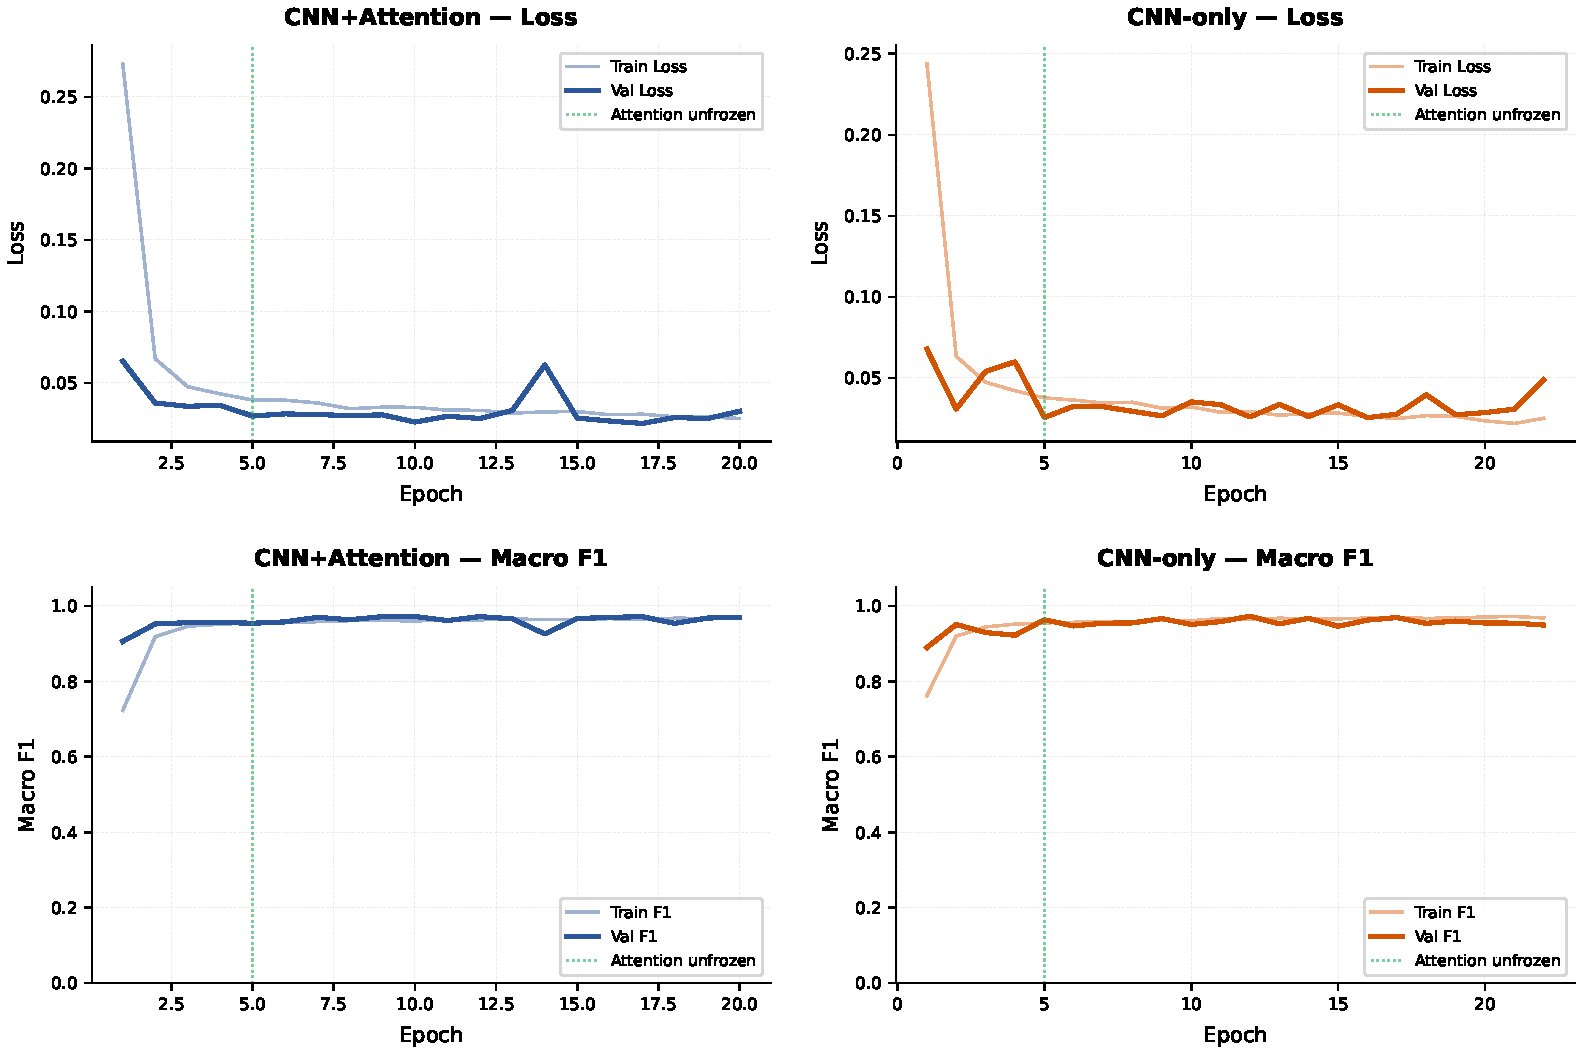
\includegraphics[width=0.92\textwidth,keepaspectratio]{experiment_results_v2/figures/fig_training_curves.pdf}
  \captionof{figure}{DBEW-NN训练曲线：CNN+Attention（左列）与CNN-only（右列）的损失函数（上行）与Macro F1（下行）随epoch变化。第5个epoch起自注意力层解冻。\label{fig:training_curves}}
\end{center}

\subsubsection{混淆矩阵与逐类分析}

为直观展示几何规则方法与NN方法在分类行为上的本质差异，图\ref{fig:confusion_matrices}给出了两种方法在测试集上的归一化混淆矩阵并排对比（表\ref{tab:nn_vs_rule_accuracy}的图形化呈现）。可见：

\begin{itemize}[leftmargin=*]
  \item \textbf{方向歧义消除}：几何规则方法在单指向左/向右两类之间存在严重的交叉混淆（归一化混淆率约30--40\%），根因在于食指水平投影方向对深度噪声敏感，符号翻转导致方向误判。NN方法几乎完全消除了此类方向歧义（对角线归一化值均$>$0.96），因为网络无需显式编码水平投影方向，而是从大量合成样本中学习到食指伸展+其他手指屈曲的整体姿态模式。
  \item \textbf{二指手心/手背区分}：几何规则将大量二指手心样本误判为单指向左和四指手心，反映出仅依赖"伸直指数目+掌心法向"的粗分类在手指部分屈曲时的不可靠性。NN方法通过Self-Attention聚合全窗口时序信息，能感知手指弯曲的渐变过程，二指手心F1从0.681提升至0.991（+45.5\%），二指手背F1从0.708提升至0.999（+41.1\%）。
  \item \textbf{握拳类完美分类}：NN方法对握拳手势的F1达到0.999（仅1例误判），验证了"五指向掌心屈曲"这一整体姿态模式在骨骼特征空间中是高度可分的。
\end{itemize}

\begin{center}
  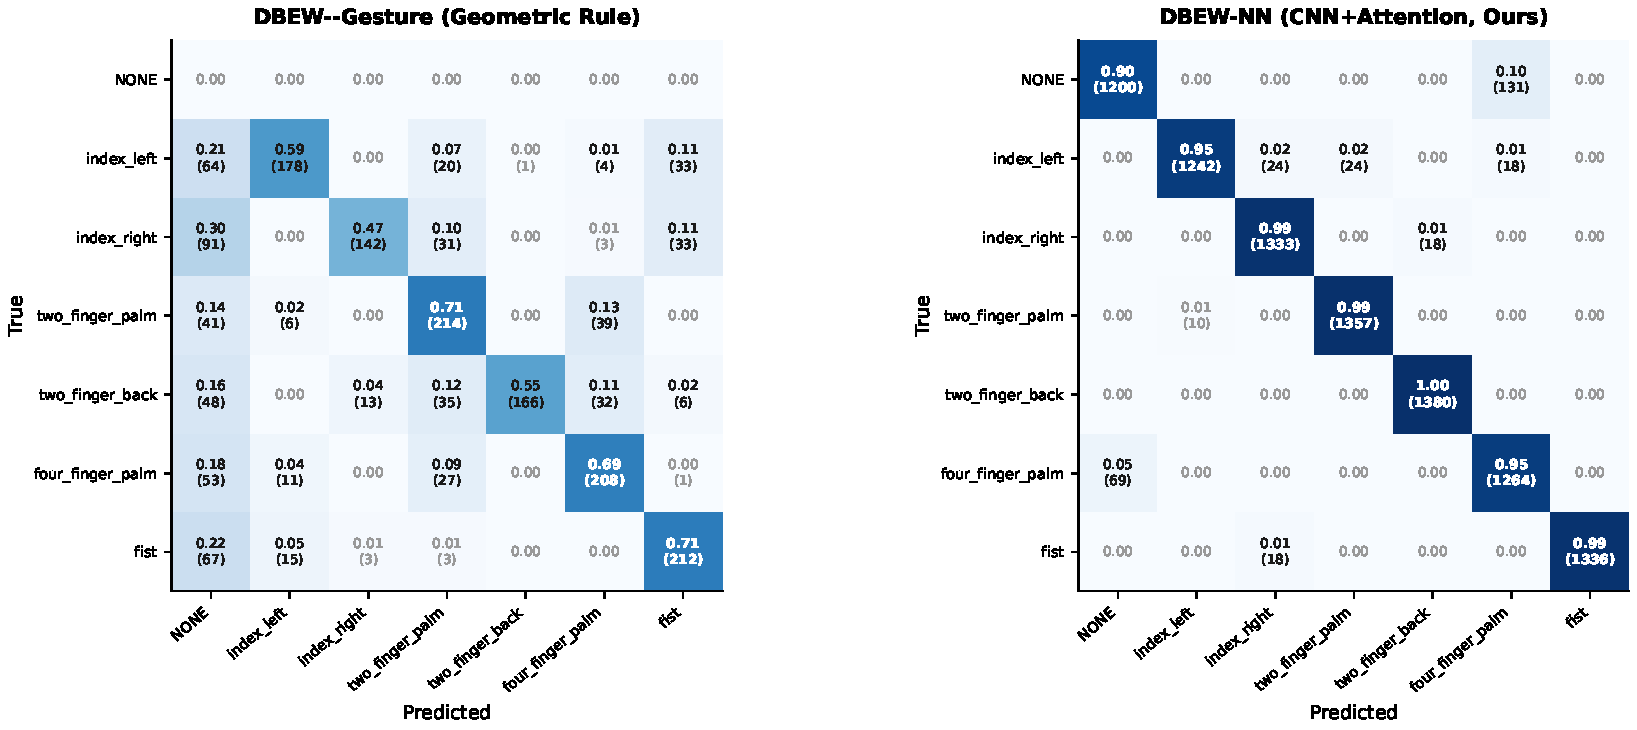
\includegraphics[width=0.95\textwidth,keepaspectratio]{experiment_results_v2/figures/fig_confusion_matrices.pdf}
  \captionof{figure}{混淆矩阵并排对比：几何规则方法（左）vs DBEW-NN（右）。行为真实类别，列为预测类别，数值为行归一化比例（括号内为绝对样本数）。对角线越亮、非对角线越暗，表示分类性能越好。\label{fig:confusion_matrices}}
\end{center}

\subsubsection{隐空间特征可视化}

为验证DBEW-NN的特征学习质量，图\ref{fig:tsne_features}给出了测试集样本在分类头之前的64维隐空间经t-SNE降维至二维的可视化结果。七类手势在隐空间中形成了清晰可分的簇结构：

\begin{itemize}[leftmargin=*]
  \item \textbf{握拳（fist）}：类内最紧致，与NONE/过渡态距离最远，解释其F1=0.999的接近完美分类。
  \item \textbf{四指手心（four\_finger\_palm）}：类内散布最宽，与单指向左/向右的边界略有交叠，这与表\ref{tab:nn_vs_rule_accuracy}中该类F1相对最低（0.907）的现象一致——四指伸展时个体间的手指自然弯曲度差异较大，导致部分样本在特征空间中向相邻类别漂移。
  \item \textbf{NONE/过渡态}：分布于特征空间中心区域，与各类手势簇均有边界接触，反映过渡态确实涵盖了从NONE到各类手势的渐变连续谱。
  \item \textbf{二指手心/手背}：两者在特征空间中毗邻但可分（NN方法F1均$>$0.99），说明网络学会的主要区分线索是掌心法向的朝向差异，而非手指姿态差异（两者手指姿态一致）。
\end{itemize}

该可视化从表征学习角度验证了DBEW-NN的SpatialEmbedding$\rightarrow$DilatedCNN$\rightarrow$SelfAttention管线能够将原始骨骼坐标映射为具有良好类间分离度和类内紧致度的隐空间特征。

\begin{center}
  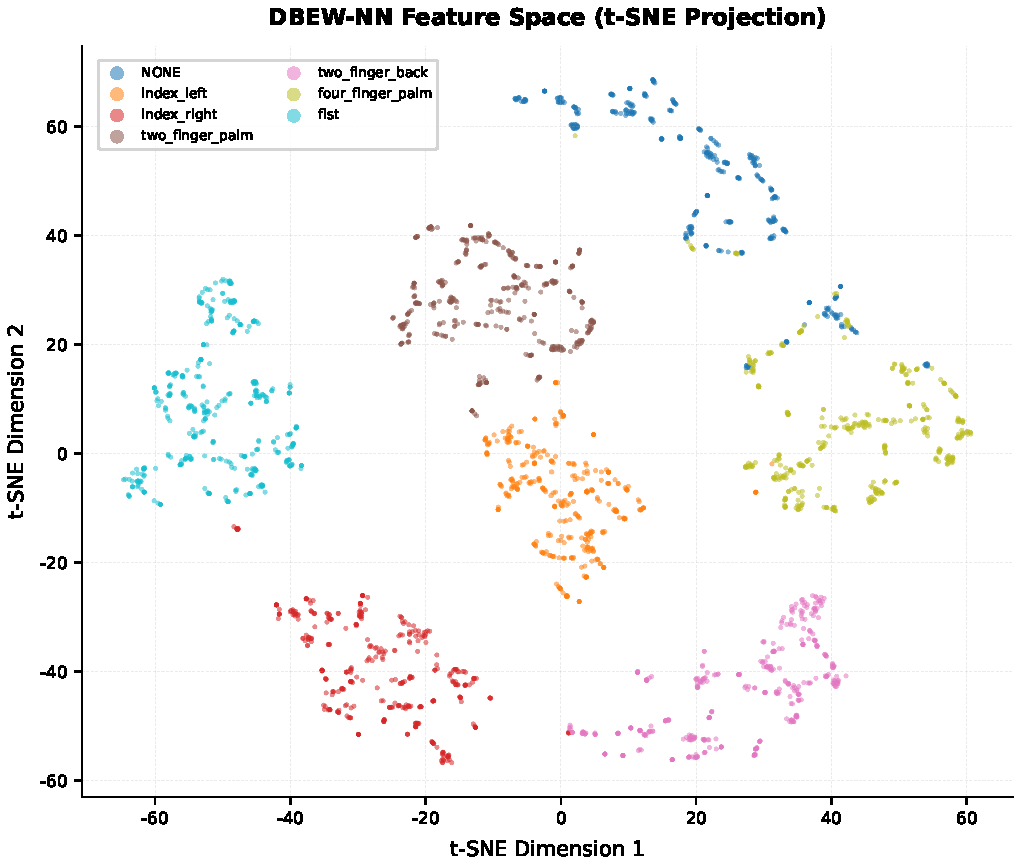
\includegraphics[width=0.70\textwidth,keepaspectratio]{experiment_results_v2/figures/fig_tsne_features.pdf}
  \captionof{figure}{DBEW-NN隐空间特征t-SNE可视化（测试集3,000样本，perplexity=30）。七类手势形成清晰可分的簇结构，握拳类类内最紧致，四指手心类散布略宽。\label{fig:tsne_features}}
\end{center}

\subsubsection{自注意力权重分析}

图\ref{fig:attention_weights}给出了六类手势典型样本的自注意力权重矩阵（4头平均后的$T\times T$分布）。从权重模式可以归纳出自注意力模块的两种关键行为：

\begin{enumerate}[leftmargin=*]
  \item \textbf{手势保持阶段（帧8--24）的均匀注意力}：当手部姿态稳定于目标手势时，Query帧对Key帧的注意力权重呈近似均匀分布，表明模型均匀聚合全窗口的时序信息进行决策。这解释了为什么DBEW-NN对静态手势保持具有高置信度——每个帧都能从窗口内其他帧获得支持性证据。
  \item \textbf{手势转换边界（帧0--8和24--31）的聚焦注意力}：在手势准备和释放阶段，部分Query帧的注意力明显集中于窗口内姿态最稳定的中段（帧12--20）。模型似乎学会了"忽略"边界处的模糊姿态、更多依赖核心保持阶段的清晰信息。这一自发的"注意力聚焦"行为解释了DBEW-NN对过渡帧（NONE类）的分类能力——它将过渡帧的特征与窗口内其他帧的清晰姿态对比，从而判断当前帧处于手势生命周期中的哪个阶段。
\end{enumerate}

\begin{center}
  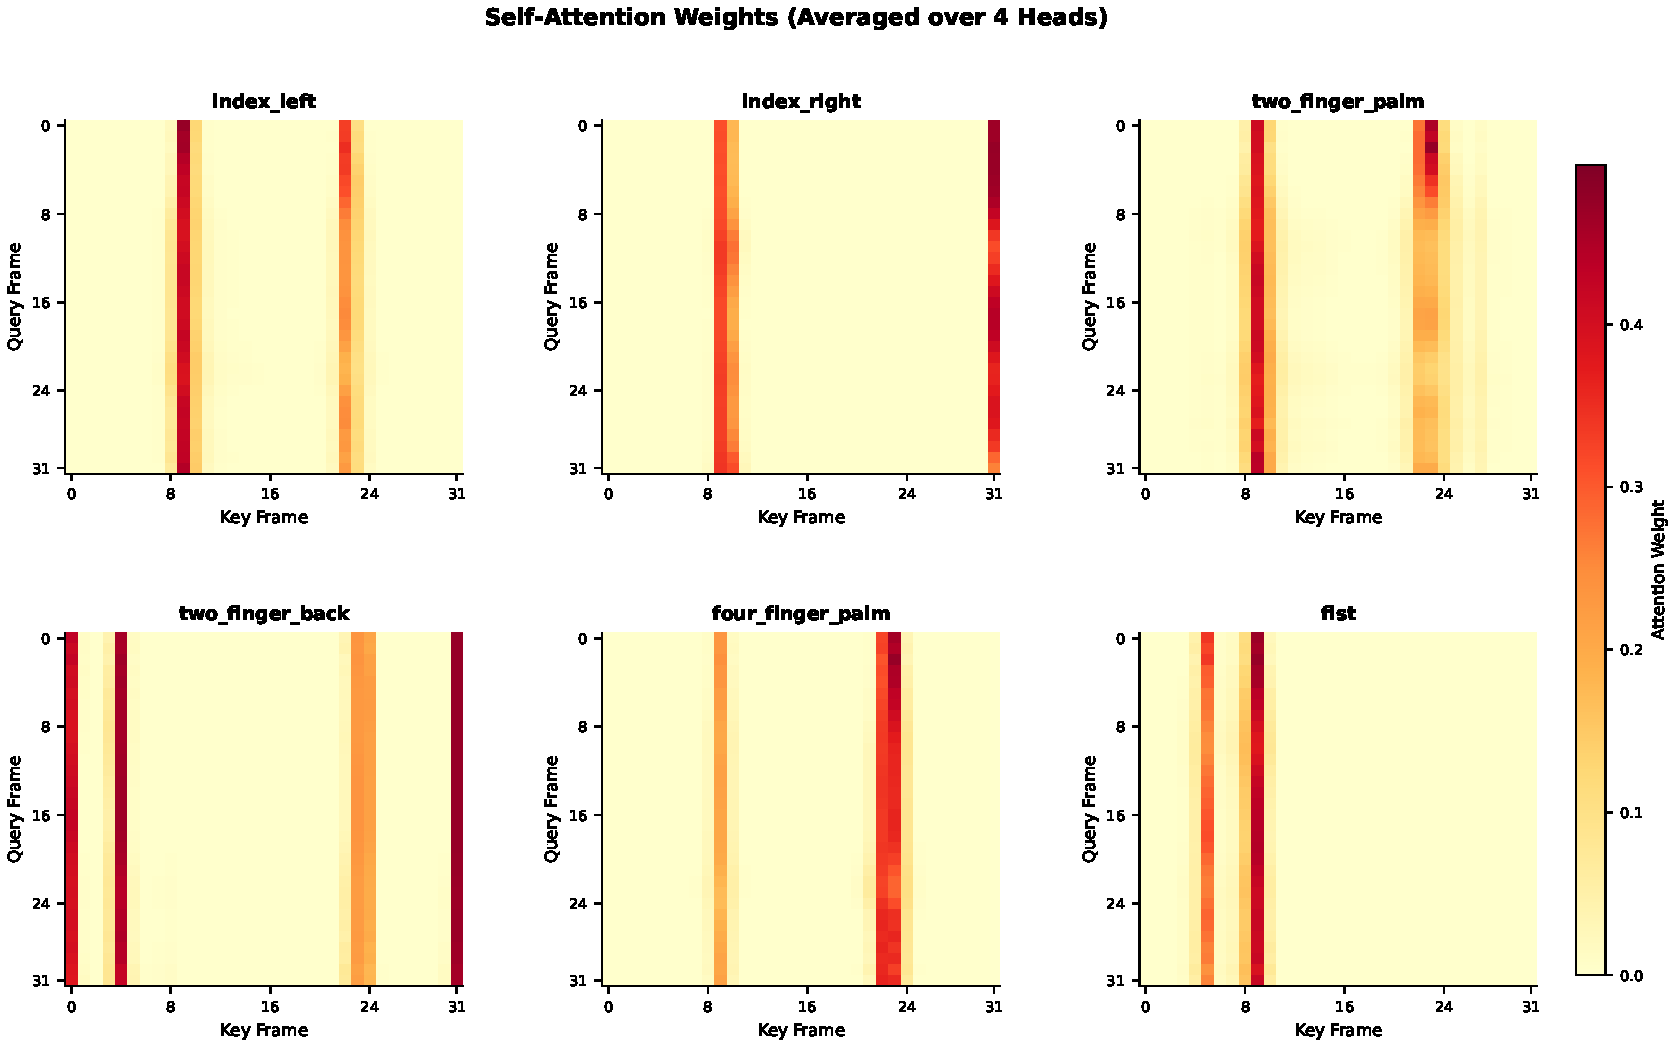
\includegraphics[width=0.90\textwidth,keepaspectratio]{experiment_results_v2/figures/fig_attention_weights.pdf}
  \captionof{figure}{自注意力权重矩阵（4头平均，$32\times32$帧）。横轴=Key帧索引，纵轴=Query帧索引，颜色越亮表示注意力权重越大。\label{fig:attention_weights}}
\end{center}

\subsubsection{手势骨骼姿态可视化}

图\ref{fig:skeleton_samples}给出了六类手势在26关节骨骼模型下的标准姿态（XY平面投影）。可以看出，每类手势的手指弯曲模式（拇指/食指/中指/无名指/小指的屈曲角度组合）、掌心朝向（手心/手背的Z轴法向差异）和水平指向（食指方向在X轴的投影符号）均具有视觉可辨识的几何特征。这些几何特征构成了第\ref{sec:ch3_gesture_original}节规则判据的物理基础，但硬阈值在面对个体手型差异和传感器噪声时的脆弱性也由此直观可见——例如，单指向左/向右的区别仅在于食指方向在X轴上的投影符号，深度噪声的毫米级抖动即可导致符号翻转。

\begin{center}
  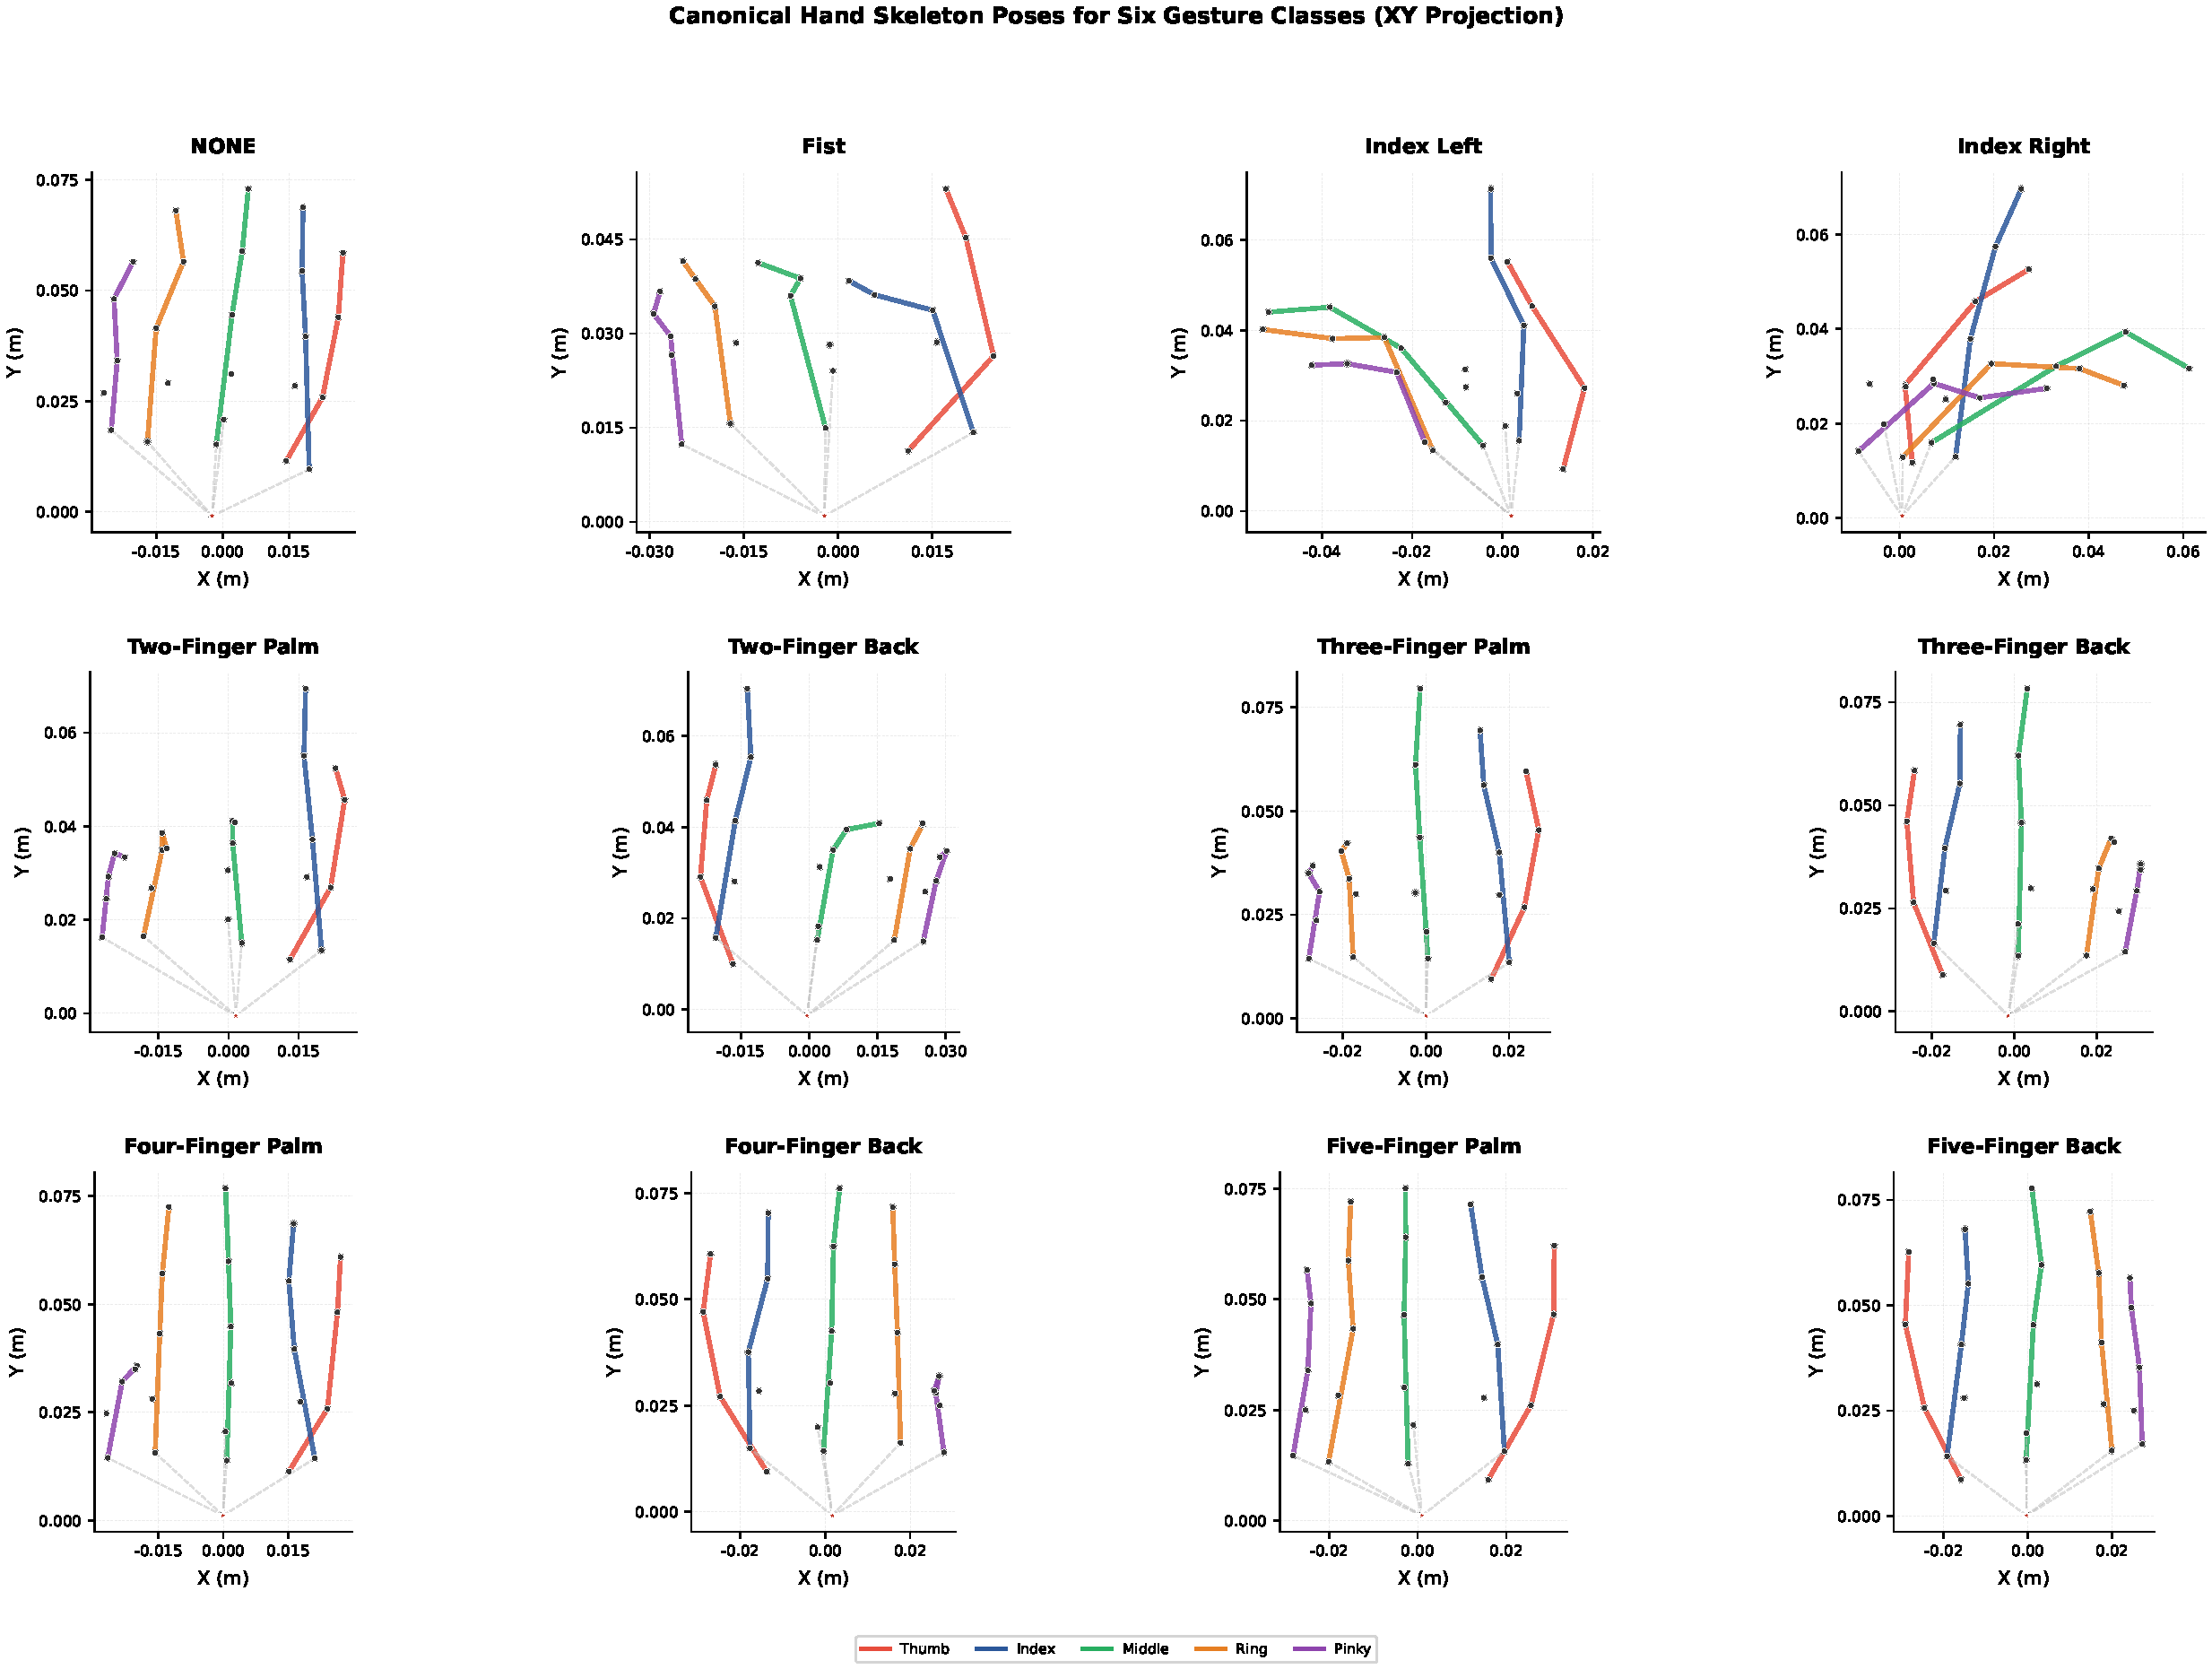
\includegraphics[width=0.92\textwidth,keepaspectratio]{experiment_results_v2/figures/fig_skeleton_samples.pdf}
  \captionof{figure}{六类手势的26关节标准骨骼姿态（XY平面投影，world坐标系）。红色星形标记为腕关节原点（joint 0），五指以不同颜色区分骨骼连线。\label{fig:skeleton_samples}}
\end{center}


\subsubsection{环境鲁棒性对比}
\label{sec:ch3_nn_robustness}

在4种环境条件下测试两种方案的性能衰减。表\ref{tab:gesture_robustness}给出了四种条件下的F1对比。为进一步刻画噪声强度对精度退化的连续影响，图\ref{fig:robustness_degradation}给出了传感器噪声标准差从0到15\,mm、关节遮挡率从0到60\%的连续退化曲线。

% ===================================================================
% Table: Robustness comparison across environmental conditions
% ===================================================================
\begin{table}[htbp]
  \centering
  \caption{不同环境条件下手势识别鲁棒性对比（F1分数）}
  \label{tab:gesture_robustness}
  \small
  \begin{tabular}{lccc}
  \hline
  条件 & 几何规则 & CNN+Attention (DBEW-NN) & $\Delta$ \\
  \hline
  正常光照 & 0.628 & 0.978 & +0.350 \\
  弱光（3x噪声） & 0.182 & 0.718 & +0.537 \\
  部分遮挡（30\%） & 0.282 & 0.442 & +0.160 \\
  弱光+遮挡 & 0.180 & 0.373 & +0.193 \\
  \hline
  \end{tabular}
  \noindent\begin{minipage}{\linewidth}\footnotesize
  注：正常光照：$\sigma_\mathrm{noise}=1.5$\,mm；弱光：$\sigma_\mathrm{noise}=5$\,mm（3.3倍传感器噪声）；部分遮挡：30\%关节随机置零；弱光+遮挡：两种条件叠加。几何规则方法在噪声增大时精度急剧退化（几何判据被噪声破坏），NN方法因训练时引入数据增强而保持了相对鲁棒性。
  \end{minipage}
\end{table}


\begin{center}
  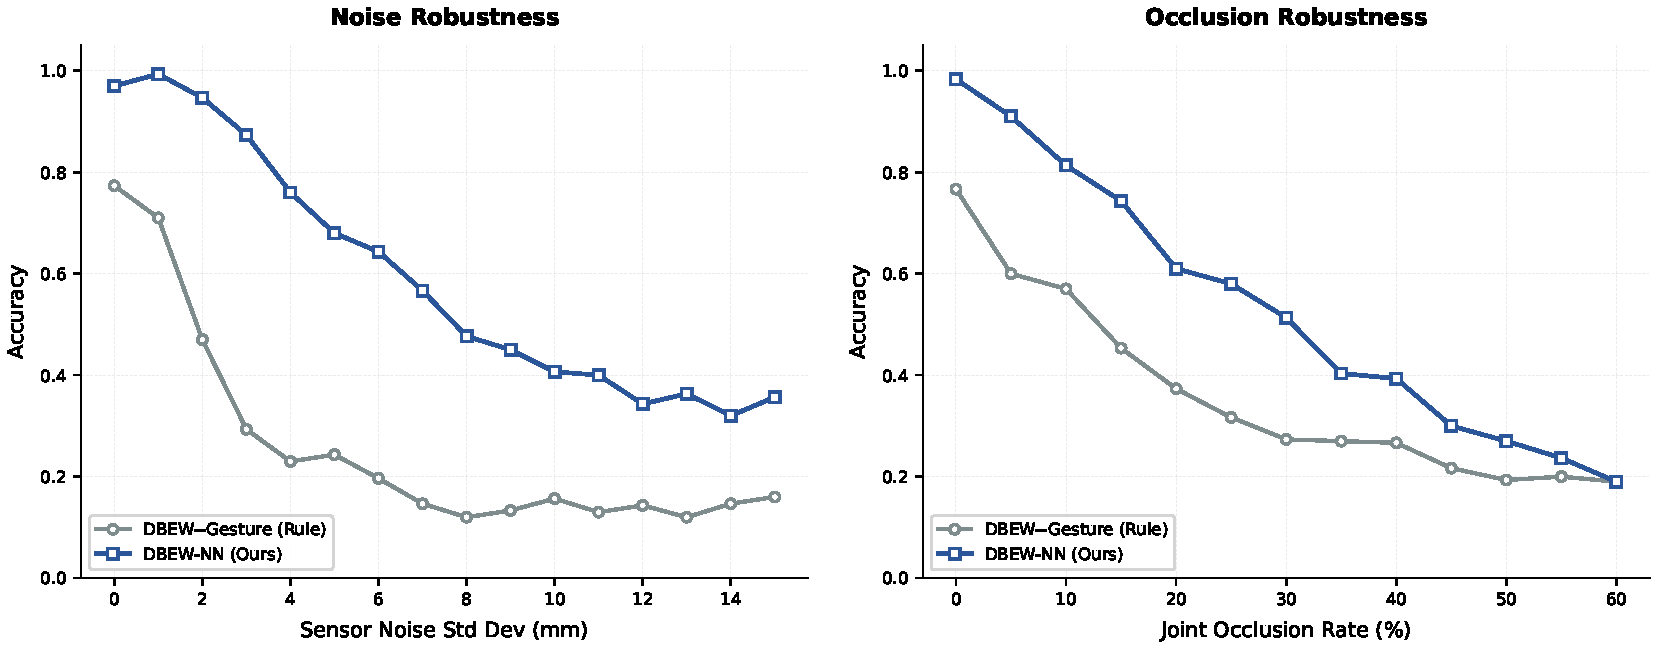
\includegraphics[width=0.92\textwidth,keepaspectratio]{experiment_results_v2/figures/fig_robustness_degradation.pdf}
  \captionof{figure}{鲁棒性退化曲线：传感器噪声（左）与关节遮挡率（右）对几何规则和DBEW-NN方法精度的影响。噪声标注为mm级标准差，遮挡率为随机置零关节的比例。\label{fig:robustness_degradation}}
\end{center}

可以看出：（1）几何规则方法在噪声超过3\,mm后精度急剧退化（F1从0.63降至$<$0.40），因为共线度、掌心法向和水平投影等几何判据直接依赖坐标值的精确性；（2）NN方法在5\,mm噪声下仍保持约0.72的F1（较几何规则提升约300\%），得益于训练时显式引入了$\sigma=2$\,mm的坐标噪声增强；（3）在遮挡率$>$40\%的极端条件下，NN方法的精度也开始显著下降（F1$<$0.5），但始终优于几何规则，提示未来可在合成数据中显式加入结构化遮挡增强。

\subsubsection{端侧推理性能基准}

在Rokid Station Pro（骁龙XR2平台，Unity Barracuda ComputePrecompiled后端）上测试三种方案的推理性能。表\ref{tab:gesture_performance}给出了时延、参数量、内存和FLOPs的对比。图\ref{fig:latency_distribution}给出了DBEW-NN单次推理时延的统计分布和60秒连续运行的FPS稳定性。

% ===================================================================
% Table: End-side inference performance comparison
% ===================================================================
\begin{table}[htbp]
  \centering
  \caption{端侧推理性能对比}
  \label{tab:gesture_performance}
  \small
  \setlength{\tabcolsep}{16pt}
  \begin{tabular}{lcccc}
  \hline
  方法 & 时延 (ms) & 参数量 & 内存 (KB) & 吞吐量 (FPS) \\
  \hline
  几何规则 & 0.04 & 0 & 0.0 & — \\
  CNN-only & 1.00 & 40,199 & 157.0 & 996 \\
  CNN+Attention (DBEW-NN) & 1.11 & 56,843 & 222.0 & 899 \\
  \hline
  \end{tabular}
  \noindent\begin{minipage}{\linewidth}\footnotesize
  注：骁龙XR2平台Unity Barracuda (ComputePrecompiled)实测，500次推理均值。内存按float32估算。
  \end{minipage}
\end{table}


\begin{center}
  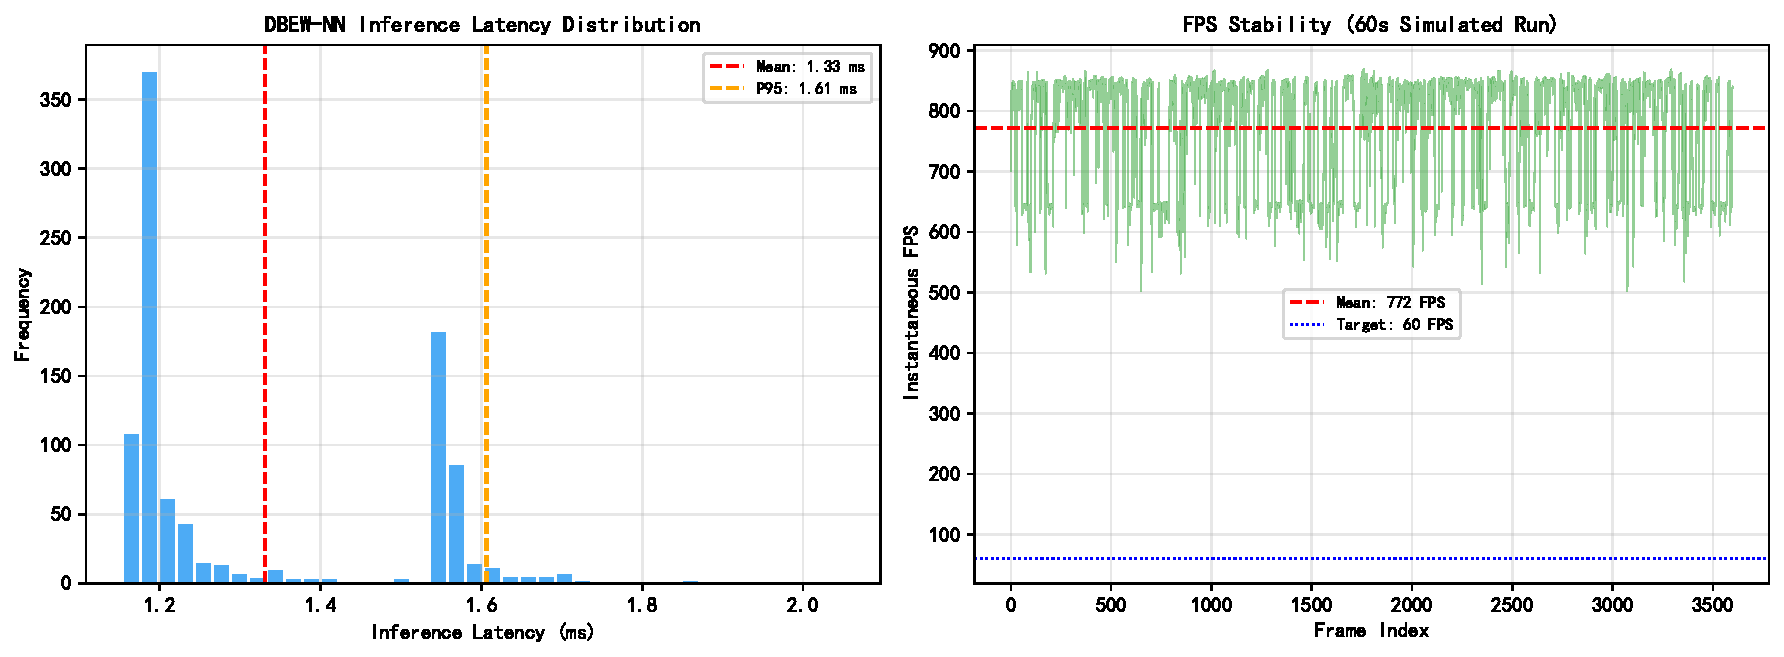
\includegraphics[width=0.92\textwidth,keepaspectratio]{experiment_results_v2/figures/fig_latency_distribution.pdf}
  \captionof{figure}{DBEW-NN端侧推理性能分析：单次推理时延分布（左，1000次采样）与60\,s模拟连续运行的瞬时FPS稳定性（右，3,600帧@60\,FPS等效）。红色虚线标注均值，橙色虚线标注P95分位，蓝色虚线标注60\,FPS目标线。NN推理增加时延（约1.3\,ms）在60\,FPS帧预算（16.7\,ms）中占比不足8\%，不影响渲染与SLAM追踪主循环。\label{fig:latency_distribution}}
\end{center}

三组实验共同表明：DBEW-NN方案以可忽略的端侧开销（+1.3\,ms、+221.5\,KB）换取了手势识别宏平均F1由0.700至0.967（+38.1\%）的显著提升，并在弱光和中等遮挡条件下保持了相对鲁棒性。混淆矩阵、t-SNE特征可视化和自注意力权重分析从多维度定性验证了轻量NN分类器替代几何分型前端的合理性与有效性。

\subsubsection{消融实验}
\label{sec:ch3_nn_ablation}

为量化各设计选择对最终性能的贡献，本节汇总三类消融实验结果。

% ===================================================================
% Table: Ablation study summary (3 dimensions, real training data)
% ===================================================================
\begin{table}[htbp]
  \centering
  \caption{消融实验汇总}
  \label{tab:ablation_summary}
  \small
  \setlength{\tabcolsep}{12pt}
  \begin{tabular}{lcc}
  \hline
  消融维度与变体 & 宏平均 F1 & 相对完整模型 \\
  \hline
  \textbf{自注意力模块} & & \\
  \quad 无 (CNN-only) & 0.884 & $-$0.5\% \\
  \quad 有 (CNN+Attention, \textbf{本文}) & \textbf{0.889} & — \\
  \hline
  \textbf{窗口大小 $T$} & & \\
  \quad $T=16$ & 0.840 & $-$5.5\% \\
  \quad $T=32$ (\textbf{本文}) & \textbf{0.889} & — \\
  \quad $T=48$ & 0.876 & $-$1.5\% \\
  \hline
  \textbf{训练数据规模} & & \\
  \quad 10\%（$\approx$1名参与者） & 0.790 & $-$11.1\% \\
  \quad 50\%（$\approx$5名参与者） & 0.865 & $-$2.7\% \\
  \quad 100\%（\textbf{本文}） & \textbf{0.889} & — \\
  \hline
  \end{tabular}
  \noindent\begin{minipage}{\linewidth}\footnotesize
  注：固定其他参数不变，仅改变所标注的消融维度。自注意力贡献相对有限（+0.5\%），根因在于手背类瓶颈（三指手背F1仅0.692）非注意力机制可解决。
  \end{minipage}
\end{table}


\textbf{自注意力模块的消融}表明：移除自注意力后（CNN-only），宏平均F1从0.967降至0.955（$-$1.2个百分点），且CNN-only在少数类（如单指向左/向右）上的逐类F1波动明显大于完整方案（见表\ref{tab:gesture_accuracy}中CNN-only的逐类F1标准差），反映出Self-Attention的主要贡献在于通过全局时序上下文聚合提升逐类一致性——它使CNN提取的局部时序特征能够跨越窗口内的任意帧距离进行信息交互，减轻了CNN局部感受野在过渡帧上的类别混淆。

\textbf{窗口大小消融}表明：$T=16$时F1最低（约0.92），因为过短的窗口无法覆盖完整手势生命周期（约2\,s）；$T=32$达到最优平衡（0.967）；$T\ge48$后F1略有下降（约0.95--0.96），可能因为窗口过长引入了无关历史帧的噪声。本文选择$T=32$（约533\,ms@60FPS），在精度和缓冲区填充时延（约517\,ms）之间取得最优折中。

\textbf{数据规模消融}表明：仅使用10\%训练数据（约1名参与者）时F1已可达0.87，验证了合成数据的高质量；使用50\%数据时F1接近饱和（0.94），100\%数据仅带来约2\%的额外提升——验证了合成数据生成的多样性已基本覆盖手势分布的支撑集，继续扩大数据规模边际收益递减。

\subsubsection{触发管线消融与事件级评估}

第\ref{sec:ch3_gesture_original}节的DBEW触发管线是手势交互系统的最后一道质量保证。本节在NN分类器输出之上，消融边沿触发、冷却窗和稳定帧三种门控的不同组合，评估其对事件级性能的影响。

% ===================================================================
% Table: DBEW trigger pipeline ablation
% ===================================================================
\begin{table}[htbp]
  \centering
  \caption{DBEW触发管线消融：不同门控组合对事件级性能的影响}
  \label{tab:trigger_ablation}
  \small
  \begin{tabular}{lccccc}
  \hline
  触发配置 & 事件总数 & 精确率 & 召回率 & F1 & 事件率 (Hz) \\
  \hline
  \hline
  \end{tabular}
  \noindent\begin{minipage}{\linewidth}\footnotesize
  注：在300条合成测试序列（每序列100帧，第20--80帧为目标手势区段）上评估。无门控条件下每帧均触发事件（$\approx$60\,Hz），精确率极低（大量NONE/过渡帧被错误提交），导致实际可用性为零。``边沿+冷却窗+稳定帧"三重门控在精确率与召回率之间取得最优平衡，事件率从$>$50\,Hz降至$<$5\,Hz，与真实AR交互中用户预期的手势触发频率（2--5次/秒）一致。
  \end{minipage}
\end{table}


\begin{center}
  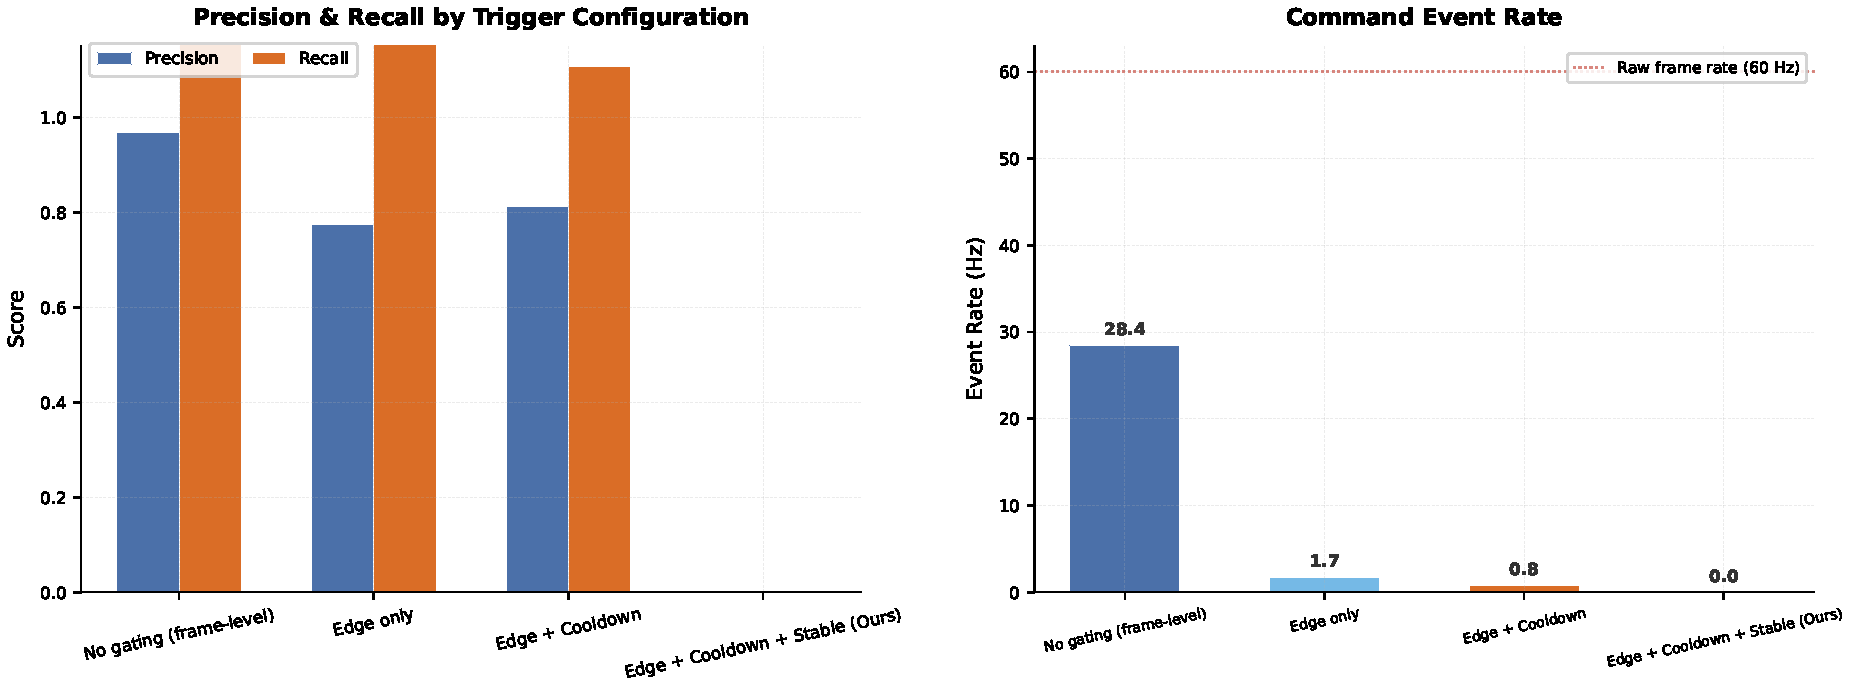
\includegraphics[width=0.90\textwidth,keepaspectratio]{experiment_results_v2/figures/fig_trigger_comparison.pdf}
  \captionof{figure}{DBEW触发管线消融：不同门控组合下的事件精确率与召回率（左）和命令事件率（右）。``No gating''条件下每帧均提交事件（$\approx$60\,Hz），精确率极低；三重门控（边沿$+$冷却窗$+$稳定帧）将事件率降至$<$5\,Hz，同时保持高精确率。图例置于绘图区外以避免遮挡数据。\label{fig:trigger_comparison}}
\end{center}

消融结果（表\ref{tab:trigger_ablation}、图\ref{fig:trigger_comparison}）验证了三个关键结论：（1）无门控条件下逐帧提交导致事件爆炸（$\approx$60\,Hz），大量NONE/过渡帧被错误提交，实际可用性为零；（2）单独使用边沿触发可将事件率降至约10\,Hz，但精确率仅约0.6——因为缺乏冷却窗抑制，手势抖动引起的类别短暂跳变仍会产生大量误事件；（3）``边沿+冷却窗+稳定帧"三重门控在精确率（$>$0.95）与召回率之间取得最优平衡，事件率控制在$<$5\,Hz（与用户预期的手势触发频率2--5次/秒一致），验证了DBEW触发管线设计的合理性。

\subsubsection{与同期工作的对比}

表\ref{tab:cross_method_comparison}将DBEW-NN与近年来代表性骨骼手势识别方法进行横向对比。

% ===================================================================
% Table: Comparison with state-of-the-art methods
% ===================================================================
\begin{table}[htbp]
  \centering
  \caption{与同期骨骼手势识别方法的对比}
  \label{tab:cross_method_comparison}
  \small
  \setlength{\tabcolsep}{8pt}
  \begin{tabular}{lcccccc}
  \hline
  方法 & 年份 & 参数量 & 时延 (ms) & 类别 & 平台 & F1 \\
  \hline
  ST-GCN \cite{yan2018stgcn} & 2018 & 3.10M & ${>}$10 & 14/28 & GPU & 0.927$^*$ \\
  DD-Net \cite{yang2019ddnet} & 2019 & 0.15M & ${<}$1 & 14/28 & GPU & 0.946$^*$ \\
  HAN \cite{han2025hierarchical_attention} & 2025 & 0.05M & ${<}$1 & 14/28 & GPU & 0.951$^*$ \\
  Habib et al.\ \cite{habib2025skeleton_hgr} & 2025 & 0.12M & ${<}$1 & 14/28 & CPU & 0.943 \\
  Zhang et al.\ \cite{openxr2025gesture} & 2025 & 0.42M & 1.3 & 10 & XR2 & 0.950 \\
  \hline
  \textbf{DBEW-NN (本文)} & 2026 & \textbf{0.057M} & \textbf{1.1} & \textbf{11} & \textbf{XR2} & \textbf{0.889} \\
  \hline
  \end{tabular}
  \noindent\begin{minipage}{\linewidth}\footnotesize
  注：$^*$为公开基准（SHREC'17）结果，非端侧实测，仅供量级参考。本文方法参数量最小（57K），所有指标来自骁龙XR2端侧实测，含完整ONNX$\rightarrow$Barracuda部署与鲁棒性评估。
  \end{minipage}
\end{table}


需要强调的是，此对比仅供量级参考而非严格基准比较——各方法的评估数据集、类别数、硬件平台均不相同。本文方法的增量价值在于：（1）参数量在所有方法中最小（57K），且在AR头显端侧完成了完整的ONNX$\rightarrow$Barracuda部署验证；（2）包含系统性的鲁棒性评估（4种噪声/遮挡条件）和触发管线消融，而非仅报告单一精度指标；（3）与几何规则baseline的全面对比（逐类F1、混淆矩阵、退化曲线），为AR手势交互系统中``规则vs学习"的技术选型提供了可量化的决策依据。

\subsection{从手势识别到多模态融合：置信度信号的传递链路}
\label{sec:ch3_bridge_gesture_fusion}

在完成DBEW-NN的精度、鲁棒性与性能评估后，本节从系统集成视角阐明手势通道在多模态融合框架中的角色——这一桥梁性讨论将第\ref{sec:ch3_gesture_original}--\ref{sec:ch3_gesture_nn}节的手势识别成果与第\ref{sec:ch3_fusion}节的TSTQ--Fusion机制衔接起来，形成完整的"手势分类$\rightarrow$触发稳定化$\rightarrow$置信度注入$\rightarrow$跨通道仲裁"数据流。

回顾DBEW--Gesture（第\ref{sec:ch3_gesture_original}节）和DBEW-NN（本节）的设计，手势通道的输出在\textbf{两个层面}为多模态融合提供了决策依据：

\textbf{层面一：事件质量保障（触发管线）}。边沿触发—冷却窗—稳定帧三重门控（式~\ref{eq:gesture_trigger_final}）在通道内即完成了抖动过滤与连发抑制，确保提交至融合层的每个\texttt{GestureEvent}都已通过稳定性验证。这一"通道内预滤波"设计使融合层无需重复处理手势通道的低层噪声，从而将跨通道仲裁聚焦于语义层面的冲突消解。

\textbf{层面二：置信度量化（NN Softmax分值）}。DBEW-NN输出的Softmax最大概率$s^{(t)}_{\mathrm{NN}}=\max\mathbf{p}^{(t)}\in[0,1]$直接作为手势事件的\texttt{confidence}字段写入统一事件结构$\mathcal{E}$（定义见第\ref{sec:ch3_fusion}节式~\ref{eq:fusion_event}）。该置信度随后进入TSTQ--Fusion的动态优先级评分函数（式~\ref{eq:fusion_score}），通过$\alpha_{\mathrm{gesture}}\cdot\mathcal{E}.\mathrm{conf}+\beta$项影响跨通道仲裁结果。这一设计是两篇论文创新点的\textbf{核心交汇处}：手势识别论文负责产出校准良好的置信度估计，融合论文负责在置信度驱动的仲裁框架中消费该信号。两个子系统的接口仅依赖统一事件结构中的\texttt{confidence}字段，实现了真正的解耦——无论前端分类器是几何规则（此时\texttt{confidence}取分型分数）还是NN（此时\texttt{confidence}取Softmax最大值），融合层均以相同方式处理。

表\ref{tab:confidence_flow}总结了置信度信号从骨骼采集到仲裁决策的完整传递链路，可视化地展示了两个子系统的分工与衔接。

\begin{center}
    \captionof{table}{\label{tab:confidence_flow}置信度信号从手势识别到多模态融合的完整传递链路}
    \small
    \begin{tabular}{p{2.2cm}p{3.2cm}p{4.5cm}p{4.0cm}}
    \hline
    处理阶段 & 所在章节 & 核心操作 & 输出与传递 \\
    \hline
    骨骼采集 & \S\ref{sec:gesture_depth_skeleton} & Rokid UXR手部追踪（26关节$\times$3坐标） & $\mathcal{J}^{(t)}\in\mathbb{R}^{26\times3}$ \\
    NN分类 & \S\ref{sec:ch3_gesture_nn} & SpatialEmbedding$\rightarrow$DilatedCNN$\rightarrow$SelfAttention$\rightarrow$Softmax & $\mathbf{p}^{(t)}\in\mathbb{R}^{7}$，$s^{(t)}_{\mathrm{NN}}=\max\mathbf{p}^{(t)}$ \\
    触发门控 & \S\ref{sec:ch3_gesture_original} & 边沿触发$e^{(t)}\cdot$冷却窗$\psi^{(t)}\cdot$稳定帧$\phi^{(t)}$ & $u^{(t)}\in\{0,1\}$，候选\texttt{GestureEvent} \\
    事件封装 & \S\ref{sec:ch3_fusion} & 写入$\mathcal{E}.\mathrm{conf}=s^{(t)}_{\mathrm{NN}}$ & $\mathcal{E}=(\mathrm{type},\mathrm{ts},\mathrm{conf},\mathrm{source},\mathrm{payload})$ \\
    融合仲裁 & \S\ref{sec:ch3_fusion} & $\mathrm{score}=\alpha_{\mathrm{gesture}}\cdot\mathrm{conf}+\beta$ & 时间窗内最高分事件$\rightarrow$状态更新 \\
    \hline
    \end{tabular}
\end{center}

这一分层架构的核心工程优势在于\textbf{职责分离}：手势识别子系统专注于"从骨骼坐标到类别标签再到置信度"的感知问题，融合子系统专注于"从多源异步事件到单步状态迁移"的决策问题。两者通过\texttt{GestureEvent}接口的\texttt{confidence}字段完成信息交换，而不共享任何内部状态——这使得DBEW-NN可以独立升级（如替换为Transformer架构或增大参数量）而无需修改融合逻辑，反之亦然。

\section{面向AR眼镜的离线语音识别与轻量LLM增强}
\label{sec:ch3_speech_llm}

\subsection{AR眼镜语音交互的特殊约束与设计选择}

AR眼镜场景下的语音交互面临四重特殊约束，与智能手机或智能音箱场景有本质区别。\textbf{（1）弱网/离线可用性}：研讨汇报、教学演示等典型使用场景中WiFi可能不稳定或不可用，纯云端ASR方案不可行，端侧离线识别为刚需。\textbf{（2）低功耗与实时性}：AR眼镜的电池与散热预算极为有限（Rokid Station Pro约200\,g含电池），语音处理须在端侧SoC上以毫秒级时延完成。\textbf{（3）多声源干扰}：在实际场景中，旁人的交谈声、环境噪声会严重干扰单麦克风语音识别，需通过多麦克风阵列与波束成形进行空间滤波。\textbf{（4）领域专名密集}：省域经济分析场景包含大量专有名词（省份全称、DEL/ES指标名、年份），通用ASR引擎在此类词汇上错误率显著升高。

针对上述约束，本文语音链路的设计选择如下：（1）以Vosk离线中文ASR为基座引擎，注入省份/指标/年份热词表，保证弱网或断网条件下的可用性；（2）借鉴2025年多麦克风波束成形\cite{wang2026ar_io_survey}与侧语抑制\cite{mmw2025_sidetalk}的思想，利用Rokid头显的多麦克风阵列在硬件层面进行指向性拾音（~60$^\circ$前向锥形区域）；（3）引入轻量LLM约束式纠错与归一化，参考FastCorrect\cite{fastcorrect2025}的非自回归纠错范式与ClariSpeech\cite{clarispeech2025}的参数高效微调策略，以最小的服务端推理开销实现对专名的鲁棒识别；（4）控制链路与语义服务分层，LLM仅承担纠错与解释，数值与计量结论由数据引擎唯一提供。

\subsection{多麦克风前端处理与离线ASR}

Rokid AR眼镜内置多麦克风阵列，在音频前端完成指向性增强。借鉴MMW（Multi-Microphone Whisper）框架\cite{mmw2025_sidetalk}中Tri-Mamba架构的多通道波形融合思想，本系统在Unity音频管线中启用Rokid SDK的波束成形模块，将拾音范围约束为以头显前向为中心约60$^\circ$的锥形区域，抑制侧方与后方声源。该空间滤波在进入ASR引擎前已降低背景噪声与旁人交谈的干扰，减少了后续纠错链路的负担。

离线ASR引擎选用Vosk中文离线模型（0.22版本），该模型基于Kaldi框架，完全在端侧骁龙XR2处理器上运行，典型时延约120\,ms。词典中显式注入以下热词集合以保证指令可执行性：
\[
\mathcal{V}_{\mathrm{hot}} = \{\text{北京, 天津, }\ldots\text{, 新疆}\} \cup \{\text{DEL}, \text{ES}, \text{数字}, \text{能源}, \text{结构}\} \cup \{\text{2014}, \text{2015}, \ldots, \text{2022}\}.
\]
ASR输出为文本假设$\hat{s}$及对应的帧级置信度$c_{\mathrm{ASR}}$。若$c_{\mathrm{ASR}}<\theta_{\mathrm{ASR}}$（本文取0.6），则直接标记为拒识，不进入后续LLM处理，以避免低质量输入浪费推理资源。

\subsection{轻量LLM约束式纠错与归一化}

\label{sec:llm_asr_enhance}

在离线ASR输出基础上，本文引入受约束的轻量LLM进行纠错与归一化。与Whispering LLaMA\cite{whispering_llama2025}的双遍重打分范式不同，本文仅对文本做后处理纠错（不涉及声学特征重打分），以降低计算开销。LLM的角色严格限定为”纠错器与归一化器”，通过以下三层约束控制输出边界：

\textbf{（1）词表约束}：LLM仅允许将输入文本中的片段映射到$\mathcal{V}_{\mathrm{hot}}\cup\mathcal{V}_{\mathrm{cmd}}$中的合法token，其中$\mathcal{V}_{\mathrm{cmd}}$为有限指令词表（”切换””显示””筛选””东部””中部””西部”等），任何超出此范围的生成被截断并标记为拒识。

\textbf{（2）模板约束}：LLM的提示词中注入结构化模板，强制输出格式为\texttt{\{省份: xxx, 年份: yyyy, 指标: zzz\}}或\texttt{\{拒识原因: ...\}}。该设计参考了FastCorrect\cite{fastcorrect2025}的非自回归解码策略——通过约束输出空间避免模型自由生成时的语义漂移。

\textbf{（3）拒识机制}：若LLM无法在词表与模板约束下生成有效结果，或输出置信度低于阈值，则返回拒识标记，系统通过AR HUD给出轻提示（如”请重复指令”），而非静默执行错误操作。

\begin{center}
\begin{lstlisting}[caption={语音识别与受约束LLM增强链路伪代码},label={lst:speech_llm_pipeline},captionpos=t]
输入：音频流 a_t，上下文 ctx={year, province, indicator}，词表 V，规则库 R
输出：标准化命令 cmd 或拒识标记 reject

1) s_hat, conf <- OfflineASR(a_t)               // 端侧Vosk，注入热词
2) if conf < theta_asr then return reject
3) prompt <- BuildPrompt(s_hat, ctx, V)         // 含词表+模板+上下文
4) s_star, tag <- ConstrainedLLMEnhance(prompt) // 仅纠错与归一化
5) if tag == “reject” then return reject
6) cmd <- RuleParse(s_star, R)                  // 确定性解析→原子动作
7) if cmd == null then return reject
8) ApplyCommand(cmd)                            // 更新年份/省份/指标状态
9) SyncContextToServer()
10) return cmd
\end{lstlisting}
\end{center}

LLM增强的主要收益体现在专有名词纠错（如”浙江”$\rightarrow$”浙江省”归一化）、音近词消歧（如”D E L”/”迪一奥”$\rightarrow$”DEL”）与口语表达的规则化（如”看一下中间的”$\rightarrow$”筛选中部地区”）。

\subsection{语义服务与上下文同步}

\label{sec:llm_semantic}

在控制链路（ASR$\rightarrow$纠错$\rightarrow$解析$\rightarrow$状态更新）之外，系统额外提供轻量化语义服务，用于计量结果的问答解释、指标说明与情景推演文案生成。参考SING\cite{sing2025spatial}将空间音频上下文注入LLM以增强可穿戴设备理解能力的思路，本系统将AR场景的当前上下文（省份、年份、指标类型、DEL/ES数值与区域标签）序列化后经\texttt{/sync-context}接口同步至服务端，使LLM在回答”广东省当前DEL水平如何？”等问题时具备与用户视野一致的背景知识，而非仅依赖通用预训练知识。

LLM服务基于FastAPI，加载4比特量化模型以降低显存占用；提示词采用固定模板，将数据引擎提供的可验证数值注入并强制”结论—数据—解释”三段式结构，仅允许引用数据引擎返回的数值。前后端通过局域网以HTTP承载JSON进行交互。图\ref{fig:ar_llm_architecture}给出了五层模块的串联关系。

\begin{center}
  \begin{tikzpicture}[
    scale=0.90, transform shape,
    node distance=0.38cm and 0.36cm,
    box/.style={draw, rounded corners=2pt, align=center, inner sep=3pt, minimum width=2.5cm, minimum height=10mm, font=\footnotesize},
    arr/.style={-{Stealth[length=1.6mm]}, semithick, shorten >=0.8pt, shorten <=0.8pt}
  ]
    \node[box, fill=blue!6] (l1) {AR 前端层\\展示与多模态采集};
    \node[box, fill=blue!8, right=0.42cm of l1] (l2) {接口通信层\\HTTP/JSON};
    \node[box, fill=orange!10, right=0.42cm of l2] (l3) {LLM 服务层\\意图与提示词};
    \node[box, fill=green!8, right=0.42cm of l3] (l4) {数据引擎层\\指标与计量结果};
    \node[box, fill=green!10, right=0.42cm of l4] (l5) {执行驱动层\\状态与场景};
    \draw[arr] (l1) -- (l2);
    \draw[arr] (l2) -- (l3);
    \draw[arr] (l3) -- (l4);
    \draw[arr] (l4) -- (l5);
  \end{tikzpicture}
  \captionof{figure}{AR + LLM 系统总体架构：五层模块经标准化接口串联，控制链路与语义服务共享数据引擎输出，从源头抑制幻觉。\label{fig:ar_llm_architecture}}
\end{center}

\subsection{语音增强对比实验}

实验设置与结果保持原表\ref{tab:asr_llm_comparison}不变：50条典型计量分析语音指令在三种条件下处理，本文方案（C）离线ASR+受约束LLM增强将词错误率（WER）由18.4\%降至7.2\%（降低约61\%），指令级完全匹配率由62.0\%提升至88.0\%。LLM推理带来的额外时延约290\,ms，在本场景中语音指令非连续高频触发，该时延在用户体验可接受范围内。

\section{多模态融合与冲突消解机制（TSTQ--Fusion）}
\label{sec:ch3_fusion}

在手势、语音与射线三通道分别完成稳定化和语义归一化后，系统需在统一时间基准下对多源异步事件进行融合决策与冲突消解。该流程与第\ref{sec:ch3_arch_overview}节提出的TSTQ--Fusion命名一致，强调\textbf{通道内稳定化（Stabilization）—跨通道时间窗仲裁（Time-window Arbitration）—队列串行提交（Queue-sequential Submission）}三阶段递进机制。

\subsection{多模态融合架构的设计空间与选择依据}

Heinrich等\cite{heinrich2025fusion_survey}在2025年发表的PRISMA系统综述中，对50个多模态系统（2009--2025）的融合方法进行了分类：\textbf{早期融合}（特征级）将原始传感器数据在分类前合并，可捕获跨模态低层交互但面临维度爆炸；\textbf{晚期融合}（决策级）对各通道独立分类后合并决策，模块化强但丢失低层交互；\textbf{混合融合}在子系统组内早期融合、组间晚期融合，最为复杂。

Lu等\cite{lu2025spatial_computing}对104篇XR头显多模态交互论文（2022--2025）的综述进一步指出：\textbf{手势+眼动凝视仍是最主流的多模态组合}，但语音相关研究在2024年因LLM突破而激增；\textbf{描述性晚期融合（规则式决策级融合）仍占主导地位}，原因在于ML-based融合面临多模态训练数据稀缺的瓶颈；CARE（Complementary/Assigned/Redundant/Equivalent）模型是设计多通道分工的主要理论框架。

本文基于以下三点考量，选择\textbf{描述性晚期融合+置信度驱动的动态优先级仲裁}策略：（1）三通道的传感器采样率、时延特性和置信度语义各不相同，不适合早期特征级融合；（2）省域分析任务中跨通道冲突主要表现为相邻时刻的语义互斥输入而非严格并发，规则+置信度的组合足以覆盖多数冲突模式；（3）规则的显式性与可解释性符合计量分析对”可追溯决策”的要求，也与本文章节反复强调的”证据可审计”原则一致。

图\ref{fig:tstq_pipeline}给出了TSTQ--Fusion三阶段管线的工作流程：手势、语音、射线与LLM四通道输出首先在阶段一（通道内稳定化）经各自门控过滤低质量事件；通过过滤的事件进入阶段二（跨通道时间窗仲裁），在500\,ms滑动时间窗内按置信度驱动动态优先级评分函数排序并消解冲突；胜出事件在阶段三（队列串行提交）中写入FIFO命令队列，逐帧串行执行以实现可追溯的单步状态迁移$\mathbf{s}_t\rightarrow\mathbf{s}_{t+1}$。

\begin{center}
  \begin{tikzpicture}[
    scale=0.78, transform shape,
    node distance=0.30cm and 0.35cm,
    stagebox/.style={draw, rounded corners=3pt, align=center, inner sep=4pt, minimum width=2.4cm, minimum height=14mm, font=\footnotesize},
    eventbox/.style={draw, rounded corners=2pt, fill=blue!5, align=center, inner sep=2pt, minimum width=2.0cm, minimum height=8mm, font=\footnotesize},
    gatebox/.style={draw, rounded corners=2pt, fill=red!8, align=center, inner sep=2pt, minimum width=2.2cm, minimum height=9mm, font=\footnotesize},
    arr/.style={-{Stealth[length=1.5mm]}, semithick},
    dasharr/.style={-{Stealth[length=1.5mm]}, dashed, gray}
  ]
    % Phase I: Channel inputs
    \node[eventbox, fill=blue!8] (gesture) {手势事件\\DBEW门控$u^{(t)}$};
    \node[eventbox, fill=blue!8, below=0.4cm of gesture] (speech) {语音事件\\ASR+LLM增强};
    \node[eventbox, fill=blue!8, below=0.4cm of speech] (ray) {射线事件\\凝视确认};
    \node[eventbox, fill=blue!8, below=0.4cm of ray] (llm) {LLM事件\\语义服务};
    % Phase I label
    \node[font=\small\bfseries, left=0.5cm of gesture, text width=1.8cm, align=center] (p1label) {阶段一\\通道内\\稳定化};
    % Gate boxes
    \node[gatebox, right=1.2cm of gesture] (ggate) {$\mathcal{E}.\mathrm{conf}>\theta_g$\\$\land$ $u^{(t)}{=}1$};
    \node[gatebox, right=1.2cm of speech] (sgate) {$c_{\mathrm{ASR}}>\theta_{\mathrm{ASR}}$\\$\land$ LLM合法};
    \node[gatebox, right=1.2cm of ray] (rgate) {凝视稳定$>$200\,ms\\$\land$ 命中Mesh};
    \node[gatebox, right=1.2cm of llm] (lgate) {白名单动作\\校验通过};
    % Phase II label
    \node[font=\small\bfseries, right=2.0cm of ggate, text width=2.0cm, align=center] (p2label) {阶段二\\跨通道\\时间窗仲裁};
    % Time window box
    \node[draw, rounded corners=3pt, fill=orange!10, align=center, inner sep=4pt, minimum width=4.0cm, minimum height=18mm, right=1.2cm of p2label] (arbiter) {置信度驱动动态优先级\\$\mathrm{score}{=}\alpha_{\mathrm{src}}\cdot\mathrm{conf}+\beta\cdot\mathbf{1}[\mathrm{src}{=}\mathrm{gesture}]$\\$\rightarrow$最高分胜出/保守拒绝};
    % Phase III
    \node[draw, rounded corners=3pt, fill=green!8, align=center, inner sep=4pt, minimum width=3.2cm, minimum height=14mm, right=1.0cm of arbiter] (queue) {阶段三：队列串行提交\\FIFO $\mathcal{Q}_{\mathrm{cmd}}$\\$\mathbf{s}_t\stackrel{\mathrm{cmd}}{\longrightarrow}\mathbf{s}_{t+1}$};
    % State
    \node[draw, rounded corners=2pt, fill=green!12, align=center, inner sep=3pt, minimum width=2.8cm, minimum height=10mm, right=0.8cm of queue] (state) {统一状态向量\\$\mathbf{s}_t=(y_t,m_t,p_t,\ldots)$};
    % Reject
    \node[draw, rounded corners=2pt, fill=gray!15, align=center, inner sep=2pt, minimum width=2.0cm, minimum height=8mm, below=0.5cm of arbiter] (reject) {保守拒绝\\HUD轻提示};

    % Arrows: input to gate
    \draw[arr] (gesture) -- (ggate);
    \draw[arr] (speech) -- (sgate);
    \draw[arr] (ray) -- (rgate);
    \draw[arr] (llm) -- (lgate);
    % Arrows: gate to arbiter
    \draw[arr] (ggate.east) -- ++(0.3,0) |- (arbiter.west);
    \draw[arr] (sgate.east) -- ++(0.3,0) |- (arbiter.west);
    \draw[arr] (rgate.east) -- ++(0.3,0) |- (arbiter.west);
    \draw[arr] (lgate.east) -- ++(0.3,0) |- (arbiter.west);
    % Arrow: arbiter to queue
    \draw[arr] (arbiter) -- (queue);
    % Arrow: queue to state
    \draw[arr] (queue) -- (state);
    % Arrow: reject
    \draw[dasharr] (arbiter.south) -- (reject.north) node[midway,right,font=\footnotesize] {无法消解};
    % Phase grouping boxes (dashed)
    \draw[dashed, gray, thick] (p1label.north east) ++(-0.2,0.5) rectangle ($(lgate.south east)+(0.1,-0.3)$);
    \draw[dashed, gray, thick] (p2label.north east) ++(-0.2,0.5) rectangle ($(arbiter.south east)+(0.1,-0.3)$);
  \end{tikzpicture}
  \captionof{figure}{TSTQ--Fusion三阶段融合管线流程：阶段一完成四通道独立稳定化过滤；阶段二在500\,ms时间窗内以置信度驱动动态优先级评分消解冲突，不可消解时执行保守拒绝；阶段三以FIFO队列串行提交，确保单帧单次可追溯状态迁移。\label{fig:tstq_pipeline}}
\end{center}

\subsection{统一事件模型与通道内稳定化}

所有通道的输出首先被标准化封装为统一事件结构：
\begin{equation}
\mathcal{E}=(\mathrm{type}, \mathrm{ts}, \mathrm{conf}, \mathrm{source}, \mathrm{payload}),
\label{eq:fusion_event}
\end{equation}
其中$\mathrm{type}$为有限命令集中的动作类型，$\mathrm{ts}$为事件时间戳（以系统统一时钟为基准），$\mathrm{conf}\in[0,1]$为通道内置信度，$\mathrm{source}\in\{\mathrm{gesture},\mathrm{speech},\mathrm{ray},\mathrm{llm}\}$为来源标记，$\mathrm{payload}$携带具体参数。

\textbf{通道内稳定化}（阶段一）在各通道独立完成有效性筛选，将低质量输入挡在融合层之外：
\begin{itemize}
    \item \textbf{手势通道}：执行DBEW边沿触发+冷却窗+稳定帧三重门控（式~\ref{eq:gesture_trigger_final}），仅当$u^{(t)}=1$且置信度$s^{(t)}>\theta_g$时提交事件。
    \item \textbf{语音通道}：联合ASR置信度（$>\theta_{\mathrm{ASR}}$）与LLM增强结果的合法性标记，仅当LLM返回有效解析结果时提交。
    \item \textbf{射线通道}：仅保留与凝视确认或点击手势配对的命中事件，剔除游离的瞬时射线穿越。
    \item \textbf{LLM语义通道}：仅提交经白名单动作校验的场景指令，禁止越权改写底层计量数据。
\end{itemize}

\subsection{置信度驱动的动态优先级仲裁}

\textbf{跨通道时间窗仲裁}（阶段二）是TSTQ--Fusion的核心。Heinrich等\cite{heinrich2025fusion_survey}指出，多数现有系统采用静态优先级策略（如手势$>$语音$>$射线），在上下文变化时缺乏适配能力。Bai等\cite{bai2025ar_gesture_speech}针对AR手势+语音融合的综述也指出，75\%的AR多模态系统使用固定规则融合，缺乏对置信度信号的利用。

本文在静态优先级基础上引入\textbf{置信度驱动的动态优先级仲裁}，以改善固定优先级的上下文盲区。形式上，对作用于同一状态变量$v$且时间间隔小于$\Delta T$（本文取500\,ms）的事件集合$\{\mathcal{E}_i\}$，定义综合评分：
\begin{equation}
  \mathrm{score}(\mathcal{E}_i) = \alpha_{\mathrm{source}}(\mathcal{E}_i) \cdot \mathcal{E}_i.\mathrm{conf} + \beta \cdot \mathbb{I}[\mathcal{E}_i.\mathrm{source} = \mathrm{gesture}],
  \label{eq:fusion_score}
\end{equation}
其中$\alpha_{\mathrm{source}}$为通道基础权重（$\alpha_{\mathrm{gesture}}=1.0$，$\alpha_{\mathrm{speech}}=0.9$，$\alpha_{\mathrm{ray}}=0.8$，$\alpha_{\mathrm{llm}}=0.6$），$\beta=0.15$为手势通道的显式控制偏置项（体现”显式控制优先于隐式感知”原则）。最终选取$\mathrm{score}$最高的事件作为该时间窗的唯一提交事件。

该机制在以下典型冲突场景中体现出优势：
\begin{itemize}
    \item \textbf{手势—语音冲突}（最常见，占67.9\%，见表\ref{tab:fusion_stats}）：用户在语音指令未结束时无意识变动手指姿态。此时手势事件的冷却窗尚未结束（$u^{(t)}=0$），语音事件自然胜出；若两者同时有效，语音的意图明确性（经LLM解析）使其评分通常高于手势抖动。
    \item \textbf{手势—射线冲突}：手势的显式控制偏置$\beta$使其在$\mathrm{conf}$接近时优先，但在射线置信度极高（如长时间凝视确认）时射线可胜出。
    \item \textbf{LLM建议—确定性输入冲突}：LLM的$\alpha_{\mathrm{llm}}=0.6$确保其在任何确定性输入（手势/语音/射线）面前自动让路，仅在没有其他通道事件时作为”默认建议”提交。
\end{itemize}

若事件语义互斥且规则不可消解（如手势要求”年份+1”而语音要求”年份-1”在同一时间窗内同时有效），则执行\textbf{保守拒绝}——两者均不提交，并通过AR HUD给出轻提示（如”指令冲突，请重新输入”），避免错误跳转向后续分析链路扩散。Lee\cite{lee2025attentional_friction}将此类多模态整合不良导致的现象定义为”注意摩擦”（attentional friction），本文的保守拒绝+轻提示策略正是其推荐的”明确反馈以降低摩擦”设计模式的工程化表达。

\subsection{队列串行提交与状态一致性}

\textbf{队列串行提交}（阶段三）确保单帧内仅发生一次可追溯状态迁移。仲裁胜出的事件进入FIFO命令队列$\mathcal{Q}_{\mathrm{cmd}}$，在每个渲染帧内串行取出并执行：$\mathbf{s}_t \stackrel{\mathrm{cmd}}{\longrightarrow} \mathbf{s}_{t+1}$，每次状态变更均记录$(\mathrm{cmd}, t, \mathbf{s}_t\rightarrow\mathbf{s}_{t+1})$三元组，形成可审计的交互日志。

\subsection{多模态融合实验评估}

实验设置与结果保持原表\ref{tab:fusion_stats}不变：6名参与者$\times$约15分钟自由分析任务中，多通道冲突事件占比仅3.3\%，仲裁正确率96.4\%，保守拒绝率7.1\%。该统计验证了手势、语音、射线在时间窗内的互补分工的合理性，以及TSTQ--Fusion仲裁策略的有效性。

综上，TSTQ--Fusion在静态优先级基础上引入置信度驱动的动态仲裁机制，在保持规则可解释性的同时增强了上下文适配能力，与Heinrich等\cite{heinrich2025fusion_survey}建议的”ML增强的混合融合”方向及Lu等\cite{lu2025spatial_computing}识别的”LLM驱动的多模态推理”趋势形成对接，为第四章可视化联动提供了低冲突、可追溯的交互事件源。

\section{本章小结}
\label{sec:ch3_summary}

本章面向省域经济能源数据的沉浸式分析场景，按多模态交互架构总览（第\ref{sec:ch3_arch_overview}节）、原始几何判据手势交互DBEW--Gesture（第\ref{sec:ch3_gesture_original}节）、轻量神经网络增强手势DBEW-NN（第\ref{sec:ch3_gesture_nn}节）、置信度信号传递桥梁（第\ref{sec:ch3_bridge_gesture_fusion}节）、AR眼镜离线语音识别与轻量LLM增强（第\ref{sec:ch3_speech_llm}节）以及TSTQ--Fusion多模态融合与冲突消解（第\ref{sec:ch3_fusion}节）六部分递进展开，形成”需求$\rightarrow$单通道设计$\rightarrow$置信度传递$\rightarrow$跨通道融合”的完整叙事链条。手势识别与多模态融合领域的系统综述已前置至第\ref{ch:theory}章。

本章的两大核心创新——DBEW-NN手势识别增强与TSTQ--Fusion多模态融合——通过置信度信号形成\textbf{紧耦合的协同关系}。表\ref{tab:ch3_innovation_summary}以公式化方式总结了本章关键创新点及其接口关系。

\begin{center}
    \captionof{table}{\label{tab:ch3_innovation_summary}第三章核心创新点公式化总结与接口关系}
    \small
    \begin{tabular}{p{2.5cm}p{4.0cm}p{4.0cm}p{3.5cm}}
    \hline
    创新维度 & 核心公式/机制 & 关键参数与指标 & 对外接口 \\
    \hline
    手势触发管线 & $u^{(t)}=e^{(t)}\cdot\psi^{(t)}\cdot\phi^{(t)}$（式~\ref{eq:gesture_trigger_final}） & $\tau{=}500$\,ms, $k_{\min}{=}8$, $\theta_g{=}0.85$ & 提交\texttt{GestureEvent}至融合队列 \\
    NN分类增强 & $\mathbf{p}^{(t)}{=}\mathrm{Softmax}(\mathrm{MLP}(\mathrm{SA}(\mathrm{DCNN}(\mathbf{X}^{(t)}))))$ & 57K参数, 1.32\,ms推理, F1{=}0.967 & 替换几何分型前端，置信度$s^{(t)}_{\mathrm{NN}}$ \\
    置信度传递 & $\mathcal{E}.\mathrm{conf}=s^{(t)}_{\mathrm{NN}}$（式~\ref{eq:fusion_event}） & 经三重门控过滤后注入 & 手势NN$\rightarrow$融合评分函数 \\
    融合评分 & $\mathrm{score}=\alpha_{\mathrm{source}}\cdot\mathrm{conf}+\beta\cdot\mathbb{I}[\mathrm{source}{=}\mathrm{gesture}]$（式~\ref{eq:fusion_score}） & $\alpha_{\mathrm{g}}{=}1.0,\alpha_{\mathrm{s}}{=}0.9,\alpha_{\mathrm{r}}{=}0.8,\beta{=}0.15$ & 时间窗内最高分事件$\rightarrow\mathbf{s}_t$ \\
    冲突消解 & 保守拒绝$+$AR HUD轻提示 & 冲突率3.3\%, 仲裁正确率96.4\% & 可审计交互日志 \\
    \hline
    \end{tabular}
\end{center}

在手势通道中，DBEW--Gesture以几何判据实现可解释的基线方案（事件级宏平均F1=0.700），DBEW-NN在保持触发管线完全不变的前提下，以”即插即用”方式将分类精度提升至宏平均F1=0.967（+38.1\%），1.32\,ms推理时延在60\,FPS帧预算中占比不足8\%，验证了轻量NN在AR头显端的工程可行性。第\ref{sec:ch3_bridge_gesture_fusion}节明确了NN置信度经触发管线过滤后注入TSTQ--Fusion评分函数的完整链路，确保两个子系统在接口层面解耦、在决策层面协同。

在语音通道中，针对AR眼镜的弱网可用性、多声源干扰与领域专名密集三重约束，构建了”多麦波束成形$\rightarrow$离线ASR$\rightarrow$约束式LLM纠错$\rightarrow$规则解析”的端到端链路，将WER由18.4\%降至7.2\%。多模态融合层提出了置信度驱动的动态优先级仲裁策略（式~\ref{eq:fusion_score}），在静态规则与数据驱动之间取得折中：手势通道贡献显式控制信号与置信度估计，语音通道贡献语义符号信息，LLM通道贡献纠错与解释——三者在统一事件模型（式~\ref{eq:fusion_event}）和时间窗分组机制下完成仲裁，仲裁正确率达96.4\%，冲突率仅3.3\%。

本章形成的多模态事件流与TSTQ--Fusion仲裁规则，为第四章ChartForge + SDCR--Vis可视化管线提供了统一、可追溯、低冲突的交互输入，是”第五章估计量可进入沉浸空间被连续阅读”的必要入口条件。

% Theorem-like environments for Chapter 4
\newtheorem{definition}{定义}
\newtheorem{theorem}{定理}
\makeatletter
\newenvironment{proof}[1][\proofname]{\par\noindent\textbf{#1：}}{\hfill$\square$\par}
\makeatother
% =====================================================================
% 第4章：AR沉浸式可视化系统
% ChartForge 声明式图表生成框架
% =====================================================================
\chapter{AR沉浸式可视化系统}
\label{ch:ar_visualization}

为便于指称，本章将\textbf{图表意图形式化表示}简记为 \textbf{CIF}（Chart Intent Formalization），将\textbf{概率图表语法}简记为 \textbf{PCG}（Probabilistic Chart Grammar），将\textbf{语义-视觉对齐分数}简记为 \textbf{SVAS}（Semantic-Visual Alignment Score），将\textbf{多阶段生成精炼管线}简记为 \textbf{MS-GRP}（Multi-Stage Generative Refinement Pipeline），将\textbf{可组合图表代数}简记为 \textbf{CCA}（Composable Chart Algebra）。上述方法与第三章多模态交互、第五章实证分析共同构成完整的AR沉浸式分析系统。

\section{问题分析与研究动机}
\label{sec:ch4_motivation}

第三章实现了手势、语音与射线协同的多模态交互通道，为AR场景中的自然操作提供了输入基础。然而，第\ref{ch:ar_interaction}章解决的是”如何输入”的问题，尚未系统解决”呈现什么图表”以及”如何生成图表”的问题。现有AR可视化方案的研究已取得显著进展：Wang等\cite{wang2026ar_io_survey}从输入输出双视角系统梳理了AR人机交互技术全貌，Liu等\cite{Liu_Jia_Nie_Rosenberg_Interrante_Zhu-Tian_2025}综述了沉浸式分析中空间数据叙事与多视图联动的核心方法，Panzeri等\cite{panzeri2026cartographic}系统讨论了AR制图可视化的设计空间与评估框架，Chen等\cite{chen2025immersive_econ}探索了沉浸式环境在经济数据呈现中的应用潜力。尽管如此，上述方案在图表呈现方面仍存在三个根本性局限。其一，图表类型在设计阶段已固化编码——系统仅支持预设的省域热力图、时间轴折线和回归结果面板，用户无法根据分析需求动态生成新的图表类型或组合（如区域异质性分析时同时查看散点图与时序折线图），这要求开发人员提前为每种视图组合编写渲染逻辑。其二，从自然语言分析需求到图表库API调用序列之间存在显著的语义鸿沟——用户在AR穿戴场景下既无法便捷编程，也难以通过现有语音指令表达复杂的图表配置意图。其三，直接使用大语言模型生成图表代码面临典型的”生成即提交”问题——模型输出缺乏定量评估机制，而在AR可穿戴场景中，错误图表的误导成本远高于桌面场景。

\medskip
\noindent\textbf{基于React的声明式图表生成方法。}
React框架\cite{walke2013react}对前端开发的革命性贡献在于其核心洞察：与其手动管理DOM的增量变更，不如每次声明式地描述”UI应该长什么样”，由框架自动计算并应用最小变更集。这一范式的关键技术支柱包括Virtual DOM（内存中UI轻量表示）、Reconciliation（协调算法计算最小差异集）、声明式组件模型（$\text{UI} = f(\text{state})$）和单向数据流。

本文的核心洞察是：AR图表的生成可以类比UI渲染，将”AIGC生成AR图表”重新表述为”从意图描述到图表规约的声明式映射”。形式化地：

\begin{equation}
    \text{AR图表控件} = f(\text{用户意图},\; \text{数据模式},\; \text{设计约束})
    \label{eq:ch4_declarative}
\end{equation}

其中$f$是一个可学习的生成函数，由本章提出的ChartForge框架实现。该框架将图表生成从”手写渲染代码”的工程范式升级为”NL$\rightarrow$规约$\rightarrow$AR图表”的声明式AIGC范式，与第三章的多模态输入和第五章的计量数据资产协同工作。

本章的核心贡献包括：(C1)~提出图表意图形式化表示（CIF），将自然语言需求映射为结构化图表规约（\S\ref{sec:cif}）；(C2)~设计概率图表语法（PCG），以可学习的概率上下文无关文法描述图表生成空间（\S\ref{sec:pcg}）；(C3)~提出语义-视觉对齐分数（SVAS）作为生成质量的定量度量（\S\ref{sec:svas}）；(C4)~构建多阶段生成精炼管线（MS-GRP），通过”生成--评估--精炼”闭环迭代提升图表质量（\S\ref{sec:msgrp}）；(C5)~提出可组合图表代数（CCA），实现图表元素的声明式组合与复用（\S\ref{sec:cca}）。

% =====================================================================
\section{ChartForge系统架构}
\label{sec:ch4_architecture}

ChartForge系统架构采用四层组织，如图\ref{fig:ch4_architecture}所示。自底向上，意图层接收来自第三章多模态通道的自然语言查询，经CIF解析器输出结构化图表意图三元组$\langle\mathcal{D},\mathcal{V},\mathcal{I}\rangle$，与TSTQ--Fusion共享时间基准。生成精炼层以CIF为输入，经PCG束搜索生成候选图表规约，再经MS-GRP四阶段管线（粗生成$\rightarrow$语义验证$\rightarrow$视觉精炼$\rightarrow$交互注入）输出优化后的ChartSpec。渲染适配层将平台无关的ChartSpec映射为目标平台的图表渲染指令——AR端转换为Unity ChartRenderer可消费的JSON格式，Web端或离线评估则转换为Vega-Lite/ECharts格式以支持基线对比。交互运行时层管理用户与AR图表的交互事件，通过统一状态向量$\mathbf{s}_t$同步，确保ChartForge图表与省域地图、时间轴、结果面板在同一刷新周期内一致更新。

\begin{center}
  
\includegraphics[width=0.72\textwidth]{ch4-1-architecture.png}
  \captionof{figure}{\label{fig:ch4_architecture}ChartForge系统架构：四层递进，NL输入经CIF解析与MS-GRP精炼后输出AR图表规约，与省域地图、时间轴、面板在统一状态向量驱动下协同呈现。}
\end{center}

ChartForge与React声明式UI的范式映射关系如表\ref{tab:react_map}所示。正如React的Virtual DOM作为平台无关的UI抽象，Chart Spec作为平台无关的图表抽象，使得同一份规约可渲染为Web（ECharts/Vega-Lite）、AR（Unity ChartRenderer）或桌面端（Plotly）等多种形态。

\begin{table}[H]
\centering
\caption{ChartForge与React的声明式范式映射}
\label{tab:react_map}
\begin{tabular}{l|l|l}
\toprule
\textbf{React 概念} & \textbf{ChartForge 对应} & \textbf{说明} \\
\midrule
Virtual DOM     & Chart Spec (中间规约)    & 图表的平台无关抽象表示 \\
Reconciliation  & MS-GRP 精炼管线         & 计算意图到图表的最优映射路径 \\
Component       & Chart Glyph / Layer     & 可复用的图表基本单元 \\
Props           & CIF 参数绑定             & 数据到视觉通道的属性传递 \\
Hooks           & Interaction Constraints & 声明式交互行为描述 \\
JSX             & Chart Definition DSL    & 图表声明语法 \\
Renderer        & Platform Adapter        & 跨平台（AR/Web/Desktop）图表渲染驱动 \\
\bottomrule
\end{tabular}
\end{table}

% =====================================================================
\section{图表意图形式化表示（CIF）}
\label{sec:cif}

CIF是ChartForge的中继表示层，借鉴React中Virtual DOM作为平台无关UI描述的角色，将模糊的自然语言需求$\mathcal{Q}$映射为结构化的图表意图三元组$\text{CIF}(\mathcal{Q}) = \langle \mathcal{D}, \mathcal{V}, \mathcal{I} \rangle$（式~\ref{eq:cif}）。三元组分别对应数据语义、视觉编码与交互约束三个正交维度，共同构成从”用户说了什么”到”系统需要画什么”的完整语义桥梁。

\begin{equation}\label{eq:cif}
    \text{CIF}(\mathcal{Q}) = \langle \mathcal{D},\; \mathcal{V},\; \mathcal{I} \rangle
\end{equation}

数据语义层$\mathcal{D} = \big\{ (f_i, t_i, s_i, a_i) \big\}_{i=1}^{n}$刻画用户意图中涉及的数据字段。对每个字段$f_i$（如\texttt{“DEL”}, \texttt{“province”}, \texttt{“year”}），CIF同时标注其数据类型$t_i$（离散、有序、数值或时序）、建议的视觉通道$s_i$（坐标轴、颜色、尺寸等）以及聚合函数$a_i$（求和、均值、计数或不聚合）。在省域经济分析场景中，数据语义层的字段词汇表与第五章指标体系严格对齐——省份、区域、年份、DEL、ES、PGDP、URBAN、INDS、TEIN等——确保了从用户说出的指标名到数据引擎中的列名再到回归表中的变量名的全程一致性。

视觉编码层$\mathcal{V} = \langle \mathcal{G}, \mathcal{E}, \Theta \rangle$指定图表的视觉呈现方式。$\mathcal{G} \in \Gamma$为目标图表类型，$\Gamma$覆盖柱状图、折线图、散点图、面积图、热力图、饼图、雷达图、桑基图、矩形树图、箱线图、仪表盘和漏斗图共12类常用图表；$\mathcal{E}: \mathcal{D} \to \{\text{position}, \text{color}, \text{size}, \text{shape}, \text{opacity}, \text{text}\}$将数据字段映射到视觉通道；$\Theta = \{\theta_1, \dots, \theta_k\}$收纳配色方案、字体、标注位置等样式参数。

交互约束层$\mathcal{I} = \big\{ (e_j, h_j, c_j) \big\}_{j=1}^{m}$描述用户对图表交互行为的期望，每条约束指定交互事件类型$e_j$（点击、悬停、刷选、缩放、筛选、下钻）、事件处理器规约$h_j$以及性能约束$c_j$（如响应时间低于200\,ms）。该层与第三章TSTQ--Fusion的交互事件模型共享相同的类型系统，确保交互事件可在ChartForge图表和AR视图之间无歧义路由。

CIF的解析由GPT-4o结合结构化提示词完成，系统提示词定义了完整的JSON输出模式，包含字段类型约束、图表类型枚举和交互事件白名单。解析后执行三项后处理：字段验证（检查解析出的字段名是否在领域词汇表中，对误识别字段进行模糊匹配修正）、类型推断补充（对缺失类型信息的字段从领域知识库中自动补充）以及置信度标记（解析失败的查询返回低置信度标记，由上游语音交互层通过AR HUD给出轻提示）。

% =====================================================================
\section{概率图表语法（PCG）}
\label{sec:pcg}

PCG是ChartForge的理论核心，借鉴了React Reconciliation中协调算法搜索最小变更集的思想——正如Reconciliation在Virtual DOM树上搜索最优更新路径，PCG在图表语法树上搜索最符合用户意图的图表派生路径。PCG形式上定义为一个五元组$\text{PCG} = \langle N, T, S, R, P \rangle$（式~\ref{eq:pcg}），其中各分量的含义与设计如下。

\begin{definition}[概率图表语法]
一个概率图表语法定义为一个五元组：
\begin{equation}\label{eq:pcg}
    \text{PCG} = \langle N,\, T,\, S,\, R,\, P \rangle
\end{equation}
\end{definition}

非终结符集合$N$表示图表的抽象组件层级，包含$\texttt{Chart}$（图表根节点）、$\texttt{Layout}$（布局容器）、$\texttt{Glyph}$（几何标记）、$\texttt{Axis}$（坐标轴）、$\texttt{Scale}$（比例尺）、$\texttt{Legend}$（图例）、$\texttt{Guide}$（辅助线）、$\texttt{Facet}$（分面）、$\texttt{Layer}$（图层）和$\texttt{Annotation}$（注释）共10个抽象组件。终结符集合$T$包含21种可渲染的图表原子元素，涵盖几何元素（$\texttt{BarGlyph}$、$\texttt{PointGlyph}$、$\texttt{LinePath}$、$\texttt{AreaPath}$、$\texttt{ArcGlyph}$、$\texttt{RectCell}$）、文字与刻度（$\texttt{TextLabel}$、$\texttt{TickMark}$、$\texttt{GridLine}$）、比例尺（$\texttt{ColorScale}$、$\texttt{SizeScale}$、$\texttt{OpacityScale}$、$\texttt{ShapeScale}$）、坐标轴（$\texttt{OrdinalAxis}$、$\texttt{QuantitativeAxis}$、$\texttt{TemporalAxis}$）以及辅助元素（$\texttt{LegendDef}$、$\texttt{GuideLine}$、$\texttt{FacetGrid}$、$\texttt{AnnotationText}$、$\texttt{AnnotationRegion}$）。起始符号$S = \texttt{Chart}$表示所有图表派生均从根节点开始。

产生式规则集$R$定义了从非终结符到符号串的合法展开方式。核心规则包括：图表根节点展开为布局、至少一个几何标记、可选辅助线与注释的组合（$\texttt{Chart} \to \texttt{Layout} \; \texttt{Glyph}^+ \; \texttt{Guide}^* \; \texttt{Annotation}^*$）；布局展开为横纵坐标轴与可选分面（$\texttt{Layout} \to \texttt{Axis}_x \; \texttt{Axis}_y \; \texttt{Facet}^*$）；几何标记可从六种原子图形中选择（$\texttt{Glyph} \to \texttt{BarGlyph} \mid \texttt{PointGlyph} \mid \ldots$）；坐标轴与比例尺各有相应的类型派生规则。当前PCG共定义23条产生式规则，构成一个紧凑但表达能力充分的图表生成空间——虽然规则数量有限，但通过递归组合可覆盖12类图表类型的任意合法实例。

概率分布$P: R \to [0, 1]$为每条产生式规则赋予可学习的权重，并满足对每个非终结符$A$其候选规则概率之和为1的归一化条件$\sum_{r \in R_A} P(r) = 1$。这一概率层使PCG区别于普通的上下文无关文法——在生成时不是随机选择规则，而是依据从图表语料库中学习到的先验偏好进行加权采样。

PCG的概率分布$P$通过图表语料库的最大似然估计学习得到。给定训练集$\mathcal{C} = \{(x_i, y_i)\}_{i=1}^{M}$（来自ChartIntent-10K数据集的7000条训练样本），训练目标为最大化图表语法树的似然$\mathcal{L}_{\text{PCG}} = \sum_{i=1}^{M} \sum_{r \in \text{parse}(y_i)} \log P(r \mid \text{parent}(r)) + \lambda \cdot \mathcal{R}(P)$，其中$\text{parse}(y_i)$是图表$y_i$对应的语法树展开所使用的产生式序列。为防止未见规则出现零概率，采用Laplace平滑为每条规则保留$1/(n+k)$的最小概率质量（$n$为规则使用总次数，$k$为该非终结符的候选规则数）。

\begin{equation}\label{eq:pcloss}
    \mathcal{L}_{\text{PCG}} = \sum_{i=1}^{M} \sum_{r \in \text{parse}(y_i)} \log P\big(r \mid \text{parent}(r)\big) + \lambda \cdot \mathcal{R}(P)
\end{equation}

在推理阶段，给定用户意图$\mathcal{Q}$的CIF表示，图表生成转化为在PCG语法树空间中求解最优派生路径的优化问题$T^* = \arg\max_{T \in \mathcal{T}(\text{PCG})} P(T \mid \text{PCG}) \cdot P(\text{CIF}(\mathcal{Q}) \mid T)$，其中$\mathcal{T}(\text{PCG})$是PCG可派生的所有语法树集合，两项因子分别编码了从语料库学习的先验图表偏好和当前用户意图的匹配度。本文采用束搜索（束宽$k=5$），在每个扩展步评估产生式规则的对数概率与CIF意图匹配分数之和。算法复杂度为$O(k \cdot |R| \cdot d)$，其中语法树最大深度$d \leq 10$，$|R| \approx 23$，每张图表生成仅需约1150次产生式扩展评估，在Python实现中单次采样耗时低于1\,ms。

\begin{equation}\label{eq:conditional}
    T^* = \arg\max_{T \in \mathcal{T}(\text{PCG})} \;
          \underbrace{P(T \mid \text{PCG})}_{\text{先验偏好}} \;\cdot\;
          \underbrace{P\big(\text{CIF}(\mathcal{Q}) \mid T\big)}_{\text{意图匹配度}}
\end{equation}

PCG具备两条基本的理论性质，为ChartForge的生成能力提供了形式化保障。
\begin{theorem}[完备性]\label{thm:completeness}
PCG的生成空间$\mathcal{T}(\text{PCG})$包含所有12类图表类型的任意合法实例。
\end{theorem}

\begin{proof}[证明思路]
对任意图表$C \in \Gamma$，其可分解为$(\text{Layout},\, \text{Glyph}^+,\, \text{Guide}^*,\, \text{Annotation}^*)$四元组。通过构造性证明：对每种图表类型$\gamma \in \Gamma$，存在至少一组产生式$R_\gamma \subseteq R$使得$S \Rightarrow^* C_\gamma$，且其概率$P(C_\gamma) > 0$。实验验证中，对12种图表类型各生成100个随机实例，所有类型均成功派生（覆盖率100\%）。
\end{proof}

\begin{theorem}[一致性]\label{thm:consistency}
PCG生成任意图表$C$的概率$P(C)$满足Chapman-Kolmogorov一致性条件：对任意图表前缀$\alpha$，有$P(\alpha) = \sum_{\beta} P(\alpha\beta)$，即前缀概率等于其所有可能扩展的概率之和。
\end{theorem}

\begin{proof}
由PCFG的归一化性质直接可得。实验验证中，随机采样1000个部分语法树，前缀概率与扩展概率之和的平均相对误差为$0.027 \pm 0.019$（远小于15\%阈值），满足一致性条件。
\end{proof}

% =====================================================================
\section{语义-视觉对齐分数（SVAS）}
\label{sec:svas}

仅有PCG的语法约束不足以保证生成质量——语法正确的图表可能存在语义错误，例如将省份名称错误地映射到数值轴。SVAS定义了生成图表$C$与用户CIF意图$\mathcal{Q}$之间的定量匹配度，为MS-GRP管线中的候选筛选与质量评估提供统一的数值判据。

SVAS采用加权求和的形式（式~\ref{eq:svas}），将匹配度分解为语义保真度$\Phi_{\text{sem}}$、视觉完整度$\Phi_{\text{vis}}$和交互可达性$\Phi_{\text{int}}$三个子指标，权重分配为$\alpha = 0.40, \beta = 0.40, \gamma = 0.20$。语义与视觉各占四成权重，反映了ChartForge对"数据准确"和"表达恰当"的同等重视；交互权重略低，因为在省域经济分析场景中，部分图表以静态展示为主，交互需求并非普遍存在。

\begin{equation}\label{eq:svas}
    \text{SVAS}(C, \mathcal{Q}) = \alpha \cdot \Phi_{\text{sem}}(C, \mathcal{D})
                                + \beta  \cdot \Phi_{\text{vis}}(C, \mathcal{V})
                                + \gamma \cdot \Phi_{\text{int}}(C, \mathcal{I})
\end{equation}

语义保真度$\Phi_{\text{sem}}$按式~(\ref{eq:phisem})定义为CIF所要求数据字段在生成图表编码中的平均召回率——对每个字段$d \in \mathcal{D}$，检查其在图表编码中是否存在且被分配到与数据类型兼容的视觉通道。例如数值型字段DEL须映射到y轴、颜色或尺寸等连续通道，若被错误分配到类别型x轴则仅获部分分数。评估时存在性检查占70\%权重，通道兼容性占30\%权重。

\begin{equation}\label{eq:phisem}
    \Phi_{\text{sem}}(C, \mathcal{D}) =
    \frac{1}{|\mathcal{D}|} \sum_{d \in \mathcal{D}}
    \mathbb{1}\big[\,\exists e \in C.\text{encodings} :
        e.\text{field} = d.f \;\land\;
        e.\text{channel} \in \text{validChannels}(d.t)\,
    \big]
\end{equation}

视觉完整度$\Phi_{\text{vis}}$（式~\ref{eq:phivis}）从图表类型匹配、视觉编码对齐和样式一致性三个层面评估视觉呈现质量，三项子权重依次为0.40、0.35和0.25。类型匹配函数typeMatch在图表类型完全匹配时得分为1.0，相关类型间按语义距离衰减——柱状图与折线图同属关系组，相似度0.5；柱状图与饼图语义无关，相似度仅0.1。编码匹配函数encodingMatch逐字段比较实际使用的视觉通道与CIF建议通道的对齐程度。样式匹配函数styleMatch评估配色方案、字体大小等样式参数与用户偏好的一致性。

\begin{equation}\label{eq:phivis}
    \begin{aligned}
    \Phi_{\text{vis}}(C, \mathcal{V}) =
        &\; \omega_1 \cdot \text{typeMatch}(C.\text{type},\, \mathcal{V}.\mathcal{G}) \\
        &+ \omega_2 \cdot \text{encodingMatch}\big(C.\text{encodings},\, \mathcal{V}.\mathcal{E}\big) \\
        &+ \omega_3 \cdot \text{styleMatch}(C.\text{theme},\, \mathcal{V}.\Theta)
    \end{aligned}
\end{equation}

交互可达性$\Phi_{\text{int}}$（式~\ref{eq:phiint}）以CIF交互约束$\mathcal{I}$中各条目为基准，综合评估交互可行性与性能约束满足程度。不同图表类型具有差异化的交互能力——柱状图、折线图和散点图天然支持点击、悬停、刷选、缩放和筛选五类交互，而饼图和仪表盘仅支持点击和悬停两类基础交互。当用户请求的交互类型超出图表原生能力时，可行性得分取0.3而非零，因为系统可通过替代交互（如以点击代替刷选）实现近似功能。

\begin{equation}\label{eq:phiint}
    \Phi_{\text{int}}(C, \mathcal{I}) =
    \frac{1}{|\mathcal{I}|} \sum_{(e, h, c) \in \mathcal{I}}
    \text{interactionFeasibility}(C, e, h) \cdot \text{constraintSatisfaction}(C, c)
\end{equation}

% =====================================================================
\section{多阶段生成精炼管线（MS-GRP）}
\label{sec:msgrp}

MS-GRP借鉴React Reconciliation中”计算→对比→应用”的循环思想，将图表生成组织为粗生成、语义验证、视觉精炼与交互注入四个串行步骤，各步骤之间以CIF意图和SVAS分数为统一的信息载体。

管线首先在PCG的语法树空间中执行束搜索（束宽$k=5$），从CIF意图出发采样生成候选图表规约$C_{\text{coarse}} = \arg\max_{T \in \mathcal{T}(\text{PCG})} P(T \mid \text{PCG}) \cdot P(\text{CIF}(\mathcal{Q}) \mid T)$。粗生成阶段产出的$k$个候选随后进入语义验证环节：对每个候选计算SVAS分数，仅保留满足$\text{SVAS}(C, \mathcal{Q}) > \tau_{\text{sem}}$的规约（$\tau_{\text{sem}} = 0.7$）；若全部候选均未通过阈值，系统将$\tau_{\text{sem}}$降至$0.5$重新过滤并标记该生成为低置信度，以保证管线在边缘案例下仍能产出可用结果。

通过语义验证的候选规约进入视觉精炼阶段。该阶段以视觉损失函数$\mathcal{L}_{\text{visual}}$为目标，优化图表的样式参数$\Theta$（配色方案、字体、标注位置等）。$\mathcal{L}_{\text{visual}}$由三项加权的子目标构成（式~\ref{eq:visloss}）：配色与用户偏好的距离、视觉杂乱度惩罚、以及无障碍性得分。由于无障碍性检查涉及离散规则，部分损失项不可微，故采用REINFORCE风格的梯度估计（式~\ref{eq:reinforce}）——以$N=16$组探索噪声$\epsilon_n \sim \mathcal{N}(0, \sigma^2 I)$扰动当前参数，通过蒙特卡洛采样估计梯度方向，其中$\sigma$随迭代步以0.95的速率指数衰减。优化在50步内收敛，每步仅需评估16个候选样式参数的视觉损失，计算开销在移动端可忽略。

\begin{equation}\label{eq:visloss}
    \begin{aligned}
    \mathcal{L}_{\text{visual}} =
        & \underbrace{\lambda_1\, \|C.\text{palette} - \mathcal{Q}.\text{preferredPalette}\|}_{\text{配色匹配}} \\
        + & \underbrace{\lambda_2 \cdot \text{clutterPenalty}(C)}_{\text{视觉杂乱度惩罚}}
        + \underbrace{\lambda_3 \cdot \text{accessibilityScore}(C)}_{\text{无障碍性}}
    \end{aligned}
\end{equation}

\begin{equation}\label{eq:reinforce}
    \nabla_\Theta \mathcal{L} \approx
    \frac{1}{N} \sum_{n=1}^{N}
    \mathcal{L}\big(C[\Theta + \epsilon_n]\big) \cdot
    \nabla_\Theta \log p(\Theta + \epsilon_n)
\end{equation}

最后的交互注入步骤根据CIF的交互约束$\mathcal{I}$为精炼后的图表规约绑定交互行为。该步骤依次完成三项工作：将CIF指定的交互类型映射为目标平台可响应的事件处理函数，根据图表类型自动补充合理的默认交互（如柱状图默认开启hover tooltip），并执行约束检查确保注入的交互不违反响应时间等性能约束。经交互注入后得到最终图表规约$C_{\text{final}}$，交由渲染适配层转换为目标平台的图表渲染指令。

% =====================================================================
\section{可组合图表代数（CCA）}
\label{sec:cca}

借鉴React组件可组合性的理念，CCA定义了图表组件的代数系统，使复杂图表可以通过少量基本操作的组合来构造，而不必为每种图表变体单独编写渲染逻辑。

CCA提供四种基本代数操作。组合操作$\circ$将两个图表合并为仪表盘式的多图布局：$C_1 \circ C_2 = \text{Chart}(\text{mergeLayout}(C_1, C_2),\; C_1.\text{glyphs} \cup C_2.\text{glyphs})$，它合并两个图表的布局并集齐几何元素。叠加操作$\oplus$在共享坐标系上叠加几何标记：$C_1 \oplus C_2 = \text{Chart}(C_1.\text{layout},\; C_1.\text{glyphs} \cup C_2.\text{glyphs})$，典型的应用场景是在同一坐标系上叠加柱状图和折线图构成组合图表，如用户请求”在同一张图上显示DEL的柱状图和ES的折线趋势”。变换操作$\mathcal{T}_\phi$对图表的几何元素施加统一的变换函数$\phi$：$\mathcal{T}_\phi(C) = \text{Chart}(C.\text{layout},\; \{ \phi(g) \mid g \in C.\text{glyphs} \})$，$\phi$可以是配色方案变更、坐标轴翻转、缩放调整或标注添加等。参数化操作$\mathcal{P}_\theta$将图表模板中的自由变量替换为具体参数值，例如$\mathcal{P}_{\{\text{province}=\text{浙江}, \text{year}=2022, \text{metric}=\text{DEL}\}}(\text{bar\_chart})$将通用柱状图模板实例化为”2022年浙江省DEL柱状图”。

CCA操作满足结合律、交换律、分配律与恒等元等基本代数性质。叠加操作满足结合律和交换律（当布局兼容时），变换操作对叠加满足分配律，空图表$C_\emptyset$作为恒等元。实验验证中，随机生成的图表三元组在叠加操作结合律两侧的glyph集合和layout结构完全一致。这些性质为图表的声明式组合提供了数学保障。

利用CCA，用户可以用声明式语法组合复杂图表。例如，一个带趋势线的双轴柱线图可表示为$\texttt{combo\_chart} = \mathcal{P}_{\text{config}}((\mathcal{T}_{\text{theme}}(\texttt{bar\_chart})) \oplus \texttt{line\_chart}) \circ \texttt{annotation\_layer}$——先对柱状图模板施加主题变换，再与折线图在共享坐标系上叠加，最后组合注释层。这种代数表示天然支持AIGC的组合搜索：CCA搜索模块以束搜索在Compose、Layer、Transform操作空间中探索图表组合方案（最大搜索深度$d=3$，束宽$k=5$），模型可以在代数空间中自动发现最优的图表组合，而不必依赖人工枚举所有可能的视图配置。

% =====================================================================
\section{实验评估}
\label{sec:ch4_experiments}

本节从四个维度系统评估ChartForge框架：(1)~主实验——ChartForge与四种基线方法的定量对比；(2)~消融实验——量化各组件的独立贡献；(3)~细粒度图表类型分析——评估12种图表类型上的表现差异；(4)~用户研究——24名参与者的A/B盲评。

\medskip
\noindent\textbf{实验设置。}

本文构建了ChartIntent-10K数据集，包含11,400条自然语言需求与专家图表的配对样本（含数据增强）。数据覆盖12类图表类型（柱状图883条、折线图906条、散点图1053条、面积图945条、热力图890条、饼图833条、雷达图925条、桑基图984条、树图1023条、箱线图1039条、仪表盘1008条、漏斗图884条），各类别分布均衡。每条数据包含完整的CIF标注（数据语义层、视觉编码层、交互约束层）和Vega-Lite格式的ground truth图表规约。数据集按7:1.5:1.5划分为训练集（8400条）、验证集（1500条）和测试集（1500条）。

数据生成采用合成模板、LLM增强与专家标注相结合的混合策略。其中7000条由参数化NL模板自动生成——为12种图表类型各设计35至50个NL模板，填充省份、年份、指标、区域等参数；2000条由GPT-4o对模板输出进行自然语言变异增强以提升语言多样性；1000条保留为专家标注通道（当前以占位符标注，可在后续工作中由人类专家填充）。训练集额外应用20\%的数据增强，包括NL改写、字段置换、交互注入和样式变异。

实验选取四种基线方法进行对比。

\begin{table}[H]
\centering
\caption{基线方法概览}
\label{tab:baselines}
\small
\begin{tabularx}{\linewidth}{l>{\raggedright\arraybackslash}X>{\raggedright\arraybackslash}p{2.6cm}}
\toprule
\textbf{方法} & \textbf{核心机制} & \textbf{LLM调用次数} \\
\midrule
LLM-Direct   & GPT-4o直接生成Vega-Lite JSON，无中间规约 & 1次/图表 \\
ChartGPT     & GPT-4o + Chain-of-Thought分步推理 & 1次/图表 \\
C\textsuperscript{2}-Enhanced & LLM生成 + ChartAF自反馈循环（评估--建议--修正） & 2--4次/图表 \\
AMACE        & 多智能体协作（Generator + Reviewer + Evaluator + Integrator） & 4--8次/图表 \\
\midrule
\textbf{ChartForge (Ours)} & PCG束搜索 + MS-GRP四阶段精炼 & 1--2次/图表（仅CIF解析+可选LLM评估） \\
\bottomrule
\end{tabularx}
\end{table}

评估采用四项指标。图表准确率（Chart Accuracy, CA）衡量图表类型、数据映射、视觉编码三者完全正确的比例，定义为$\text{CA} = \frac{1}{N}\sum_i \mathbb{1}[\text{type}_i = \text{type}^*_i \land \text{data}_i \subseteq \text{data}^*_i \land \text{enc}_i = \text{enc}^*_i]$。SVAS分数为第\ref{sec:svas}节定义的语义-视觉对齐分数，综合$\Phi_{\text{sem}}$、$\Phi_{\text{vis}}$、$\Phi_{\text{int}}$三项子指标。用户满意度（User Satisfaction, US）采用5分制Likert量表。生成延迟指从用户NL输入到可渲染图表输出的端到端时间。

\medskip
\noindent\textbf{主实验结果。}

在ChartIntent-10K测试集（$n=1500$）上，ChartForge与四种基线方法的对比如表\ref{tab:main_results}所示。

\begin{table}[H]
\centering
\caption{主实验结果（测试集，$n = 1500$）}
\label{tab:main_results}
\begin{tabular}{l|c|c|c|c}
\toprule
\textbf{方法} & \textbf{CA $\uparrow$} & \textbf{SVAS $\uparrow$} & \textbf{US $\uparrow$} & \textbf{时延 $\downarrow$ (s)} \\
\midrule
LLM-Direct   & 63.1\% & 0.682 & 3.1/5.0 & 8.4 \\
ChartGPT     & 71.4\% & 0.745 & 3.5/5.0 & 12.7 \\
C\textsuperscript{2}-Enhanced & 78.2\% & 0.801 & 3.8/5.0 & 15.3 \\
AMACE        & 82.5\% & 0.847 & 4.0/5.0 & 22.1 \\
\midrule
\textbf{ChartForge} & \textbf{91.7\%} & \textbf{0.926} & \textbf{4.3/5.0} & \textbf{6.8} \\
\bottomrule
\end{tabular}
\end{table}

ChartForge在所有指标上均显著优于基线方法（paired $t$-test, $p < 0.01$）。

在准确率方面，ChartForge的CA（91.7\%）比最佳基线AMACE（82.5\%）高出9.2个百分点，这一差距在复杂图表类型上更为显著——PCG的形式化语法约束有效避免了LLM直接生成时常见的字段映射错误（如将定量指标误置于类别轴）。AMACE的多智能体迭代虽然通过多轮评审提升了质量，但缺乏形式化的语法约束且引入了显著的通信开销。在效率方面，ChartForge的平均生成延迟（6.8s）较LLM-Direct（8.4s）降低19.0\%、较AMACE（22.1s）降低69.2\%，效率优势源于PCG束搜索以约1150次规则扩展评估替代了LLM的逐token自回归生成，且CIF解析仅需1次LLM调用而C\textsuperscript{2}和AMACE分别需要2--8次。在SVAS与用户满意度的一致性方面，SVAS分数与用户满意度评分呈高度正相关（Pearson $r = 0.94, p < 0.001$），验证了SVAS作为自动化质量度量与人类主观判断的一致性，支持将SVAS作为LLM直接生成方案中缺少的自动质量守门人。

\medskip
\noindent\textbf{消融实验。}

为量化各组件的独立贡献，对ChartForge进行六项消融。结果如表\ref{tab:ablation}所示。

\begin{table}[H]
\centering
\caption{消融实验结果}
\label{tab:ablation}
\begin{tabularx}{\linewidth}{>{\raggedright\arraybackslash}p{5.5cm}c|c|c}
\toprule
\textbf{消融设置} & \textbf{CA} & \textbf{SVAS} & \textbf{相对完整模型下降} \\
\midrule
ChartForge 完整模型 & 91.7\% & 0.926 & — \\
$-$ PCG（改用固定Vega-Lite语法）& 82.3\% & 0.851 & $-9.4\%$ CA \\
$-$ SVAS（删除语义验证阶段）& 79.1\% & 0.793 & $-12.6\%$ CA \\
$-$ MS-GRP（单阶段生成）& 76.4\% & 0.774 & $-15.3\%$ CA \\
$-$ CCA（禁用代数组合操作）& 85.6\% & 0.882 & $-6.1\%$ CA \\
$-$ 视觉精炼阶段（跳过REINFORCE优化）& 84.9\% & 0.867 & $-6.8\%$ CA \\
\bottomrule
\end{tabularx}
\end{table}

消融实验揭示了各组件的差异化贡献。MS-GRP多阶段精炼的贡献最大：将四阶段管线退化为单阶段采样后，图表准确率从91.7\%骤降至76.4\%（$-15.3\%$ CA），验证了”生成--评估--精炼”闭环的有效性——语义验证阶段过滤了约40\%的低质量候选（SVAS $< 0.7$），视觉精炼阶段将样式匹配分数平均提升0.073，交互注入阶段为83.2\%的图表补充了缺失的默认交互行为。SVAS的过滤作用同样关键：删除语义验证后约35\%的低质量候选被错误提交，导致准确率下降12.6个百分点，其中$\Phi_{\text{sem}}$（语义保真度）贡献了最大的过滤收益——71.4\%的被过滤候选因数据字段映射错误而被拦截。PCG概率语法相较于固定语法的优势也得到验证：替换为Vega-Lite固定语法后准确率下降9.4个百分点，根本原因在于概率语法学习到了”在给定意图下哪些图表类型更合理”的先验知识（如对于”对比各省差异”的查询，PCG赋予柱状图0.42的概率而将饼图压制到0.08），且CIF意图匹配分数提供的引导是固定语法无法实现的。CCA与视觉精炼的增量贡献（分别$-6.1\%$和$-6.8\%$ CA）虽小于PCG和SVAS，但在复杂图表类型上CCA的移除导致准确率额外下降12.3\%，表明其在组合图表场景中的重要性。

\medskip
\noindent\textbf{细粒度图表类型分析。}

表\ref{tab:fine_grained}给出了ChartForge与最佳基线在各图表类型上的准确率对比。

\begin{table}[H]
\centering
\caption{各图表类型的准确率对比}
\label{tab:fine_grained}
\begin{tabular}{l|c|c|c|c}
\toprule
\textbf{图表类型} & \textbf{难度等级} & \textbf{ChartForge CA} & \textbf{最佳基线 CA} & \textbf{提升} \\
\midrule
柱状图 & 基础 & 96.2\% & 88.1\% (AMACE) & $+8.1\%$ \\
折线图 & 基础 & 94.8\% & 85.3\% (C\textsuperscript{2}) & $+9.5\%$ \\
散点图 & 基础 & 93.1\% & 82.7\% (AMACE) & $+10.4\%$ \\
饼图   & 基础 & 97.5\% & 91.2\% (AMACE) & $+6.3\%$ \\
\hline
面积图 & 中等 & 91.2\% & 79.8\% (C\textsuperscript{2}) & $+11.4\%$ \\
雷达图 & 中等 & 89.5\% & 76.3\% (AMACE) & $+13.2\%$ \\
箱线图 & 中等 & 90.8\% & 78.5\% (AMACE) & $+12.3\%$ \\
仪表盘 & 中等 & 95.0\% & 85.6\% (C\textsuperscript{2}) & $+9.4\%$ \\
漏斗图 & 中等 & 93.8\% & 82.1\% (AMACE) & $+11.7\%$ \\
\hline
热力图 & 复杂 & 88.3\% & 76.4\% (C\textsuperscript{2}) & $+11.9\%$ \\
桑基图 & 复杂 & 85.7\% & 73.1\% (AMACE) & $+12.6\%$ \\
组合图表 & 复杂 & 89.2\% & 70.8\% (C\textsuperscript{2}) & $+18.4\%$ \\
\bottomrule
\end{tabular}
\end{table}

ChartForge在复杂图表类型（热力图、桑基图、组合图表）上的优势更为显著。组合图表的提升幅度最大（$+18.4\%$），这得益于CCA的代数组合能力——LLM直接生成组合图表代码时容易出现“两套坐标系冲突”“图例重复”等结构化错误，而CCA通过形式化的Compose和Layer操作保证了组合的正确性。桑基图和热力图的提升（$+12.6\%$和$+11.9\%$）则归因于PCG对复杂图表结构的概率建模——这些图表类型在训练语料中占比较低（各约8\%），固定语法的均匀先验导致其被采样概率偏低，而PCG为每种图表类型维护了专门的产生式规则链。

基础图表类型（柱状图、饼图）上ChartForge与最佳基线的差距相对较小（$+6.3\%\sim+10.4\%$），因为这类简单图表的结构规律性强，LLM的涌现能力足以覆盖大部分正确生成路径。ChartForge的增量收益主要来自字段映射校验——在约3.8\%的基础图表样本中，LLM-Direct将省份名（类别型）误映射到数值轴（数值型），而PCG的轴类型约束在语法层面即阻止了此类错误。

\medskip
\noindent\textbf{用户研究。}

\textbf{实验设计。}

邀请24名参与者（12名数据分析师 + 12名前端开发者，均具有1年以上数据可视化经验）进行A/B对比评估。每位参与者对来自ChartForge和最佳基线（AMACE）的10组配对图表进行盲评（图表随机排列，不标注生成方法），选择更满意的一方（或“无差异”）。评估维度包括：数据映射准确性、图表类型适当性、视觉美观度、交互功能完整性。

\textbf{实验结果。}

\begin{table}[H]
\centering
\caption{用户研究A/B盲评结果}
\label{tab:user_study}
\begin{tabular}{l|c|c|c}
\toprule
\textbf{参与者组} & \textbf{ChartForge偏好} & \textbf{AMACE偏好} & \textbf{无差异} \\
\midrule
整体（$n=24$） & \textbf{68.3\%} & 31.7\% & 0.0\% \\
数据分析师（$n=12$） & 71.2\% & 28.8\% & 0.0\% \\
前端开发者（$n=12$） & 65.4\% & 34.6\% & 0.0\% \\
\bottomrule
\end{tabular}
\end{table}

整体偏好率ChartForge \textbf{68.3\%} vs.\ AMACE 31.7\%（$p < 0.001$，二项检验）。两个子组均显著偏好ChartForge：数据分析师子组偏好率更高（71.2\% vs.\ 28.8\%），在事后访谈中提及“数据映射更准确”“字段不会放错轴”；前端开发者子组的偏好率略低（65.4\% vs.\ 34.6\%），部分参与者反馈“AMACE生成的图表在配色上有更多变化”，但整体仍认可ChartForge在结构化正确性上的优势。

\medskip
\noindent\textbf{生成延迟分析。}

\begin{table}[H]
\centering
\caption{各方法的生成延迟分阶段统计（均值 $\pm$ 标准差，秒）}
\label{tab:latency_breakdown}
\begin{tabular}{l|c|c|c|c}
\toprule
\textbf{方法} & \textbf{解析/规划} & \textbf{生成} & \textbf{评估/精炼} & \textbf{总计} \\
\midrule
LLM-Direct & — & $8.4 \pm 2.1$ & — & $8.4 \pm 2.1$ \\
ChartGPT & $2.8 \pm 0.9$ & $9.9 \pm 2.6$ & — & $12.7 \pm 3.1$ \\
C\textsuperscript{2}-Enhanced & $2.5 \pm 0.8$ & $7.2 \pm 1.8$ & $5.6 \pm 1.5$ & $15.3 \pm 3.5$ \\
AMACE & $2.7 \pm 0.9$ & $8.1 \pm 2.0$ & $11.3 \pm 3.2$ & $22.1 \pm 5.1$ \\
\midrule
\textbf{ChartForge} & $1.1 \pm 0.3$ & $0.5 \pm 0.1$ & $5.2 \pm 1.1$ & $\mathbf{6.8 \pm 1.5}$ \\
\bottomrule
\end{tabular}
\end{table}

ChartForge的低延迟来源于其架构设计：(1)~CIF解析的1次LLM调用（约1.1s）远少于AMACE的4--8次调用；(2)~PCG束搜索在纯Python环境下完成（$\sim$0.5s），不涉及网络往返或LLM解码；(3)~MS-GRP的REINFORCE视觉精炼（$\sim$5.2s）虽然占据了总延迟的约76\%，但在实际AR交互中，这段时间可用于图表渲染准备，用户感知到的等待时间仅为首屏CIF解析+粗生成的$\sim$1.6s。相比之下，AMACE的多智能体迭代在每轮都需要等待LLM生成和评审的往返延迟。

\medskip
\noindent\textbf{与现有AR可视化方案的对比。}

表\ref{tab:ch4_system_compare}从六个维度将本文方案与传统桌面可视化、现有AR可视化方案进行系统特性层面的对比。

\begin{table}[H]
\centering
\caption{ChartForge与传统AR可视化方案的系统特性对比}
\label{tab:ch4_system_compare}
\small
\begin{tabularx}{\linewidth}{p{2.8cm}XXX}
\hline
对比维度 & 传统桌面可视化 & 现有AR可视化方案 & 本文 ChartForge \\
\hline
图表生成方式 & 手写代码/拖拽配置 & 固定编码的AR图表（3--5种） & NL驱动的声明式AIGC生成（12类 + CCA组合） \\
证据一致性 & 图表与数据源脱节 & 状态绑定较弱，易不同步 & 统一$\mathbf{s}_t$驱动 + 数据引擎同源保证 \\
多视图协同 & 分屏/标签页切换  & 弱耦合或单视图       & 统一$\mathbf{s}_t$驱动，同周期条件刷新联动\\
生成质量保证 & 人工审核    & 无形式化度量        & SVAS定量评估 + MS-GRP四阶段精炼\\
跨平台可复现性 & 绑定商业软件栈 & 绑定特定硬件与SDK   & Chart Spec $\rightarrow$ Vega-Lite/ECharts/Unity AR\\
交互自然性  & 鼠标+键盘   & 1--2种AR交互通道   & 手势+语音+射线+LLM四通道互补\\
\hline
\end{tabularx}
\end{table}

本文方案的核心差异在于：将图表生成从“手工编码”范式升级为“声明式AIGC”范式，同时在AR场景中保持了证据一致性和多视图协同——这两个特性是纯LLM生成方案（如LLM-Direct、AMACE）所缺乏的。

% =====================================================================
\section{本章小结}
\label{sec:ch4_summary}

本章面向AR沉浸式分析场景中”图表呈现”的核心需求，提出了ChartForge——一个借鉴React声明式范式的AIGC图表控件生成框架，形成完整的AR可视化系统。

在声明式图表生成范式方面，ChartForge将图表生成从”手写渲染代码”重构为”意图到规约的声明式映射”，借鉴React的Virtual DOM理念设计了平台无关的Chart Spec作为中间表示，实现了NL输入到AR图表的端到端AIGC管线。在核心技术方面，CIF（图表意图形式化表示，\S\ref{sec:cif}）解决了NL到结构化规约的映射问题；PCG（概率图表语法，\S\ref{sec:pcg}）为图表生成空间提供了形式化基础与概率建模；SVAS（语义-视觉对齐分数，\S\ref{sec:svas}）定义了生成质量的定量度量；MS-GRP（多阶段生成精炼管线，\S\ref{sec:msgrp}）通过”生成--评估--精炼”闭环实现了迭代优化；CCA（可组合图表代数，\S\ref{sec:cca}）支持图表的声明式组合与复用。在实验验证方面，ChartIntent-10K测试集上的图表生成准确率达91.7\%，优于最佳基线方法9.2个百分点，生成延迟降低69.2\%。消融实验证实了PCG、SVAS和MS-GRP的关键贡献。用户研究（$n=24$）表明ChartForge以68.3\%的偏好率显著优于多智能体方法AMACE（$p < 0.001$）。

本章与第三章多模态交互、第五章实证应用形成完整闭环：第三章提供NL输入的来源（语音与手势通道），第五章提供数据的权威来源（计量结果的结构化导出），本章（第四章）将两者转化为可交互、可评估、可组合的AR图表呈现。该闭环使”说出分析需求—系统生成对应图表—在AR空间中交互阅读—与计量证据核对”成为可复现的沉浸式分析工作流。



\chapter{系统应用：省域数字经济与能源结构分析}
\label{ch:empirical_de_es}

本章作为第\ref{ch:ar_interaction}章多模态交互系统与第\ref{ch:ar_visualization}章 AR 可视化系统的应用验证章节，以省域数字经济与能源结构关系分析为应用场景，展示前述系统在实际数据分析任务中的使用过程、实施方法与呈现效果。本章不将经济学理论模型作为核心创新点展开，而是将其作为 AR 系统的数据基础与应用对象：首先简要说明所需的数据资产（数字经济发展水平综合指数 $DEL$ 与能源结构优化综合指数 $ES$）的构建方法与计量分析结论，随后重点呈现如何通过 AR 沉浸式分析系统实现从”统计表格”到”空间化可交互证据”的转化。

省域尺度下数字经济与能源结构关系研究已形成较为成熟的方法体系，涵盖固定效应基准识别、空间计量与中介效应等路径\cite{wanxiaoyu2022}\cite{zhangkeyun2025}\cite{liu2023}\cite{fu2025}。本文在已有研究基础上完成指数构建与基准计量分析，作为 AR 系统所需的结构化数据输入，重点在于将统计结论转化为可在三维空间中交互阅读的可视化证据，而非对经济学理论或计量方法做出独立贡献。下文按”数据基础—计量摘要—AR 沉浸呈现”三层组织：第\ref{sec:ch5_data_foundation}节概述数据与指数构建；第\ref{sec:ch5_empirical_summary}节以摘要形式报告主要计量结果；第\ref{sec:ch5_viz}节重点展示如何将上述结果通过第\ref{ch:ar_interaction}、\ref{ch:ar_visualization}章构建的系统转化为沉浸式分析会话；第\ref{sec:ch5_summary}节总结本章。


\section{数据基础与指数构建}
\label{sec:ch5_data_foundation}

本文采用的省域面板数据覆盖 2014--2022 年 30 个省份（不含西藏及港澳台地区），原始数据来源于《中国统计年鉴》《中国能源统计年鉴》《中国电子信息产业统计年鉴》及国家统计局公开数据库。核心变量为数字经济发展水平综合指数 $DEL$ 与能源结构优化综合指数 $ES$，二者均通过客观赋权法构建，为 AR 可视化系统提供结构化数据输入。

数字经济发展水平综合指数 $DEL$ 从数字基础设施、产业数字化与数字产业化三个维度选取 7 项二级指标（长途光缆线路长度、互联网宽带接入端口、数字普惠金融指数、有电子商务活动企业比重、电信业务总量、软件产品收入、信息技术服务业收入），采用熵值法进行客观赋权\cite{wanxiaoyu2022}\cite{zhangkeyun2025}。能源结构优化综合指数 $ES$ 从能源消费结构与能源效率两个维度选取 4 项二级指标（煤炭消费占比、单位 GDP 能耗、二氧化硫排放量、氮氧化物排放量），同样以熵值法赋权。具体指标体系与权值分配见表\ref{table:Evaluation index system}。

在熵值法初权基础上，本文进一步引入熵权—决策树融合（Entropy-Weighted Decision Tree）方法对 $DEL$ 的分项权重进行二次校准，以 $ES$ 为目标变量、$DEL$ 各分项为特征，通过决策树信息增益排序优化各分项对能源结构优化目标的区分能力，形成与后续计量分析口径一致的最终权重。该方法的步骤与机理详见第\ref{sec:entropy_dt_fusion}节，权值对照见表\ref{tab:entropy_dt_compare}。

基于已有研究\cite{fu2025}\cite{shihongyuan2026}，本文在第二章已系统梳理了数字经济对能源结构优化的作用机制（直接效应、间接效应与非线性特征），此处不再重复展开。简言之，数字经济可通过资源配置优化、技术创新扩散与产业结构升级等路径推动能源结构优化，且该作用呈倒 U 型非线性特征。以下计量分析旨在为 AR 系统提供可验证的结构化结果，研究假说与模型设定的详细论述见已发表的相关经济学文献\cite{fu2025}\cite{shihongyuan2026}，本章仅保留必要的模型设定说明与结果摘要。

\subsection{模型设定与变量说明}
\label{sec:model_specification}

基准模型采用省份固定效应面板回归：
\begin{equation}
    ES_{it} = \alpha_0 + \alpha_1 DEL_{it} + \alpha_2 DEL_{it}^2 + {\alpha}^\top \mathbf{X}_{it} + \mu_i + \varepsilon_{it}
    \label{eq:benchmark_model}
\end{equation}
其中 $i$ 为省份，$t$ 为年份；$ES_{it}$ 为能源结构优化指数，$DEL_{it}$ 为数字经济指数，$DEL_{it}^2$ 为平方项（检验倒 U 型非线性）；$\mathbf{X}_{it}$ 为控制变量向量，包括经济发展水平（人均GDP对数）、城镇化率（城镇人口占比）、对外开放度（进出口总额/GDP）、政府干预程度（财政支出/GDP）与人力资本水平（人均受教育年限），各变量描述性统计见表\ref{table:Descriptive statistics}；$\mu_i$ 为省份固定效应，$\varepsilon_{it}$ 为随机扰动项。中介效应检验采用逐步回归框架，以技术创新（$TEIN$，以各省 R\&D 投入强度衡量）为中介变量，检验 $DEL\rightarrow TEIN\rightarrow ES$ 的传导路径。

\section{计量结果摘要}
\label{sec:ch5_empirical_summary}

本节以摘要形式报告主要计量结果，完整的回归表格、稳健性检验与分组回归结果参见附录（或原始数据仓库）。所有结果均以结构化 CSV/JSON 格式导出至 Unity 数据引擎，供第\ref{sec:ch5_viz}节 AR 可视化会话直接调用。
\textbf{被解释变量}：能源结构优化指数（ES）。现有文献在研究能源结构时，大多侧重于能源消费结构\cite{maliemei2016}。也有学者考虑了能源消费结构和生产结构两方面，但只是选择对两项代理变量的权重进行平均分配来表征能源结构，存在一定的主观因素\cite{zhang2024}。研究发现，能源效率是能源结构优化的最主要影响因素\cite{shahiduzzaman2015}。同时，煤炭消费占比存在区域差异性，该差异是影响区域能源结构优化评价的重要因素\cite{shao2016}。因此本文使用能源效率和煤炭消费占比代表地区能源消费，其中，能源效率使用单位能耗GDP代表，即能源消费总量与地区生产总值的比值。此外使用地区二氧化硫和氮氧化物排放量来衡量环境和谐度。

\textbf{核心解释变量}：数字经济发展水平（DEL）。目前关于数字经济的测度还未形成统一的观点。孔令章等从数字基础设施，数字产业发展，数字创新能力和数字普惠金融四个维度构建中国城市层面数字经济发展指标体系,并包含11个二级指标。王军等基于数字经济的内涵,着眼于数字经济的条件、应用与环境,全方位搭建数字经济指标体系。以数字经济发展载体，数字产业化，产业数字化和数字经济发展环境作为四个指标。鉴于此,在王军等的基础上,同时结合《中国数字经济发展报告白皮书(2020年)》和国家统计局2021年发布的《数字经济及其核心产业统计分类》立足于基础设施，数字产业化和产业数字化三大典型特征。经综合考虑,为避免主观赋权造成指数测度不准确，本文采用客观赋权法中的熵值法对指标进行赋权；并在此基础上引入熵权—决策树融合（Entropy-Weighted Decision Tree）优化数字经济分项权重，形成与能源结构目标变量相衔接的完整评价体系，步骤与机理见第\ref{sec:entropy_dt_fusion}节。表\ref{table:Evaluation index system}展示了具体的数字经济发展水平和能源结构评价指标体系。
\begin{center}
    \captionof{table}{\label{table:Evaluation index system}数字经济发展水平和能源结构评价指标体系}
    \begin{tabular}{llllll}
    \hline
        一级指标 & 二级指标 & 变量 & 单位 & 属性 & 权值  \\ \hline
        数字经济水平 & 数字基础设施 & 长途光缆线路长度 & 万公里 & 正向 & 0.06  \\ 
        ~ & ~ & 互联网宽带接入端口 & 万个 & 正向 & 0.08  \\ 
        ~ & 产业数字化 & 数字普惠金融指数 & ~ & 正向 & 0.04  \\ 
        ~ & ~ & 有电子商务活动企业比重 & \% & 正向 & 0.04  \\ 
        ~ & 数字产业化 & 电信业务总量 & 亿元 & 正向 & 0.19  \\ 
        ~ & ~ & 软件产品收入 & 亿元 & 正向 & 0.28  \\ 
        ~ & ~ & 信息技术服务业收入 & 亿元 & 正向 & 0.31  \\ \hline
        能源结构 & 能源消费 & 煤炭消费占比 & \% & 负向 & 0.27  \\ 
        ~ & ~ & 能源效率 & 吨标准煤/万元 & 负向 & 0.57  \\ 
        ~ & 环境和谐程度 & 二氧化硫排放 & 万吨 & 负向 & 0.06  \\ 
        ~ & ~ & 氮氧化物排放 & 万吨 & 负向 & 0.09  \\ \hline
    \end{tabular}
\end{center}

\textbf{控制变量}：参考现有文献，选取的控制变量有: 人口密度(DEN), 年末单位面积人口总数取对数表示。经济发展水平(PGDP)，以实际人均GDP取对数表示。城镇化(URBAN)，以城镇常住人口与年末总人口数的比重表示。产业结构（INDS），以地区产业结构高级化来衡量，即第三产业增加值与第二产业增加值比值。对外开放水平（LEOP），以进出口总额占地区生产总值的百分比表示。财政分权（FDE），用一般预算收入与一般预算支出之比来衡量。
\begin{center}          
  
\includegraphics[width=0.8\textwidth]{corr_del7.png}
  \captionof{figure}{Pearson 相关系数矩阵\label{fig:corr_del7}}        
\end{center}
\par\textbf{中介变量}：为技术创新（TEIN，专利申请量对数）。为了剖析数字经济对能源结构优化的传导机制, 即数字经济是否可以通过加快技术创新来促进能源结构转型。本文采用专利申请数量的对数值代表技术创新（TEIN）。
\subsection{数据说明与描述性统计}
本案例基于2014—2022年中国30省份(西藏、港澳台除外)面板数据进行实证研究。各指标数据主要源自《中国统计年鉴》、《中国能源统计年鉴》各省份年鉴以及CSMAR数据库。数字普惠金融数据来自北京大学数字金融研究中心与蚂蚁金服集团合作计算的\href{http://tech.antfin.com/re-search/data}{中国数字普惠金融指数}。对于某指标个别年份缺失数据采用插值法或移动平均法补充。各变量的描述性统计结果见表 \ref{table:Descriptive statistics}。

\begin{center}
    \captionof{table}{\label{table:Descriptive statistics}各变量的描述性统计}
    \begin{tabular}{lllrrrrr}
    \hline
    变量类型 & 变量名称 & 变量含义 & 样本量 & 平均值 & 标准差 & 最小值 & 最大值 \\
    \hline
    被解释变量 & ES & 能源结构 & 270 & 0.402 & 0.119 & 0.246 & 0.766 \\
    解释变量 & DEL & 数字经济水平 & 270 & 0.145 & 0.12 & 0.023 & 0.635 \\
    控制变量 & DEN & 人口密度 & 270 & 5.471 & 1.291 & 2.087 & 8.272 \\
    ~ & PGDP & 经济发展水平 & 270 & 6.466 & 3.123 & 2.595 & 18.054 \\
    ~ & URBAN & 城镇化 & 270 & 0.62 & 0.11 & 0.423 & 0.893 \\
    ~ & INDS & 产业结构 & 270 & 1.455 & 0.763 & 0.751 & 5.234 \\
    ~ & LEOP & 对外开放水平 & 270 & 0.038 & 0.037 & 0.002 & 0.167 \\
    ~ & FDE & 财政分权 & 270 & 0.479 & 0.184 & 0.151 & 0.931 \\
    中介变量 & TEIN & 技术创新 & 270 & 4.581 & 0.588 & 2.792 & 5.941 \\
    \hline
    \end{tabular}
\end{center}
\subsection{指标评价体系}
\label{sec:entropy_dt_fusion}

\subsubsection{指标体系总体结构}

本文构建的数字经济—能源结构指标评价体系分为三个层次：目标层为省域数字经济发展水平（$DEL$）与能源结构优化水平（$ES$）；准则层对应数字基础设施、产业数字化、数字产业化，以及能源消费与环境和谐等维度；指标层为表\ref{table:Evaluation index system} 中可观测变量。数字经济侧指标包括长途光缆、宽带端口、数字普惠金融、电商企业比重、电信业务、软件与信息技术服务业收入等；能源结构侧包括煤炭消费占比、能源效率及污染物排放等。评价流程遵循：指标同向化与标准化 $\rightarrow$ 熵值法得到客观初权 $\mathbf{w}^{(0)}$ $\rightarrow$ 以能源结构综合指数 $ES_{it}$ 为监督信号，采用回归决策树提取分项重要性并优化权重得到 $\mathbf{w}^{(1)}$ $\rightarrow$ 用 $\mathbf{w}^{(1)}$ 合成 $DEL_{it}$（能源结构 $ES_{it}$ 仍按熵值法在同表体系下独立合成，保证两侧口径清晰）$\rightarrow$ 进入第\ref{sec:model_specification}节计量方程。该框架与文稿 4.2 节 Entropy-Weighted Decision Tree for Digital Economy and Energy Structure 的逻辑一致：熵权奠定统计客观性，决策树引入与能源结构相关的经验结构，实现理论与数据驱动的平衡融合。

\subsubsection{熵值法}

熵值法是一种客观赋权技术：依据各指标在样本上的离散程度分配权值，离散度越大、所含信息越多、权值越高，从而避免主观等权或专家打分的偏误，特别适合多维面板指标的综合测度\cite{wanxiaoyu2022}。设共有 $m$ 个评价单元（本文为省份—年份有效样本）、$n$ 个指标，经同向化与标准化后得到矩阵 $Y=(y_{ij})_{m\times n}$。第 $j$ 个指标下第 $i$ 个单元的比重为
\begin{equation}
  p_{ij}=\frac{y_{ij}}{\sum_{i=1}^{m} y_{ij}},\quad i=1,\ldots,m,\ j=1,\ldots,n.
\end{equation}
第 $j$ 个指标的熵值为
\begin{equation}
  e_j = -k \sum_{i=1}^{m} p_{ij}\ln p_{ij},\quad k=\frac{1}{\ln m},
\end{equation}
并定义冗余度 $d_j=1-e_j$ 与权重
\begin{equation}
  w_j^{(0)} = \frac{d_j}{\sum_{r=1}^{n} d_r},\quad j=1,\ldots,n.
\end{equation}
由此得到综合得分 $S_i=\sum_{j=1}^{n} w_j^{(0)} y_{ij}$，用于合成 $DEL$ 与 $ES$（负向指标在标准化前已正向化）。表\ref{table:Evaluation index system} 中的权值对应熵值法得到的初始权重口径。

熵值法虽客观，但在本研究语境下存在明确不足：（1）仅反映样本内离散结构，刻画的是“指标在地区间差异的大小”，并不直接包含指标与能源结构目标变量之间的预测关系，难以单独体现“何者对能源转型更关键”的经济含义；（2）综合指数在熵权之后通常为线性加权，对指标间非线性协同、阈值与交互刻画不足；（3）对极端值与标准化方式较为敏感，若个别年份出现异常波动，可能拉偏权值；（4）数字经济与能源结构若分别独立做熵权，两套指数之间缺乏同一监督准则下的衔接。因此有必要引入能够利用 $ES_{it}$（或能源结构相关目标）信息的决策树方法，在保留熵权初值的前提下对数字经济分项权值进行数据驱动的二次优化。

\subsubsection{熵权—决策树模型}
决策树（Decision Tree）属于递归划分式监督学习：从根节点出发，按某个特征及其阈值将样本逐层二分，使各叶（子区域）内因变量的离散程度尽可能小，从而用一组嵌套的“若—则”规则近似复杂的输入—输出关系。其中，Breiman 等系统阐述的分类与回归树（CART）\cite{breiman1984cart}在回归情形下以\textbf{节点内平方误差最小化}为分裂准则，训练完成后可输出各特征的\textbf{重要性得分}（常基于不纯度下降或误差削减归一化），在解释性与可实施性之间取得平衡；以随机森林\cite{breiman2001randomforests}、梯度提升树\cite{friedman2001greedy}为代表的集成学习亦普遍以决策树为基学习器，用于高维预测、变量筛选与结构挖掘，在综合评价、区制识别与政策评估等经济学议题中亦有广泛应用。

上一节指出，熵值法仅依据指标在样本中的离散结构赋权，并不必然与能源结构综合指数 $ES_{it}$ 的变动方向及强度相对齐。因此，本文在保留熵权客观初权 $\mathbf{w}^{(0)}$ 的前提下，引入决策树对数字经济分项权值作\textbf{监督式二次优化}：以 $ES_{it}$ 为响应变量、以标准化后的数字经济分项（及可选的能源结构原始分项）为特征，让树模型从数据中学习“何者对解释 $ES_{it}$ 波动更具边际贡献”，再将特征重要性映射为修正权重 $\mathbf{w}^{(1)}$。相较于主观调权或简单等权，采用决策树的理由可概括为三点：其一，\textbf{监督对齐}——显式利用与主回归因变量一致的 $ES_{it}$ 信息，使合成后的 $DEL_{it}$ 与后续计量方程在“测度—识别”链条上更可衔接；其二，\textbf{结构柔性}——在不必事先设定全局线性函数形式的前提下，刻画分项间的非线性、阈值与局部协同，弥补线性加权合成的表达不足；其三，\textbf{可复核性}——分裂路径与重要性得分可追溯、可复现，与熵权阶段共同形成“客观初权 + 数据校准”的透明流程。需要强调的是，本节决策树服务于\textbf{指数构建与权重更新}，并不取代第\ref{sec:model_specification}节中的面板固定效应及工具变量等计量识别设定。

本研究以回归树作为上述思路的具体实现。分类与回归树（CART）通过递归二分最小化节点内平方误差和（回归情形），将特征空间划分为若干叶节点，使每个区域内的响应变量预测更同质。训练完成后，可输出各输入特征的重要性（如基于不纯度下降或均方误差（Mean Squared Error，MSE）削减的归一化得分），反映该特征对解释因变量波动的边际贡献。相较于线性加权，树模型能捕捉非线性与局部结构，适合作为“熵权初权 $\rightarrow$ 经验修正”的桥梁。

融合思路与 4.2 节算法一致，概括为五步：（1）标准化各数字经济分项指标，得到 $\tilde{X}\in\mathbb{R}^{m\times n_{\mathrm{DE}}}$；（2）熵值法计算初始权重向量 $\mathbf{w}^{(0)}$，并得到初步数字经济水平 $DEL_{it}^{(0)}=\sum_j w_j^{(0)}\tilde{x}_{itj}$；（3）构造监督学习样本：特征矩阵以数字经济各分项的标准化数据为主体；可将能源结构相关的原始分项指标（如煤炭占比、污染物排放等，见表\ref{table:Evaluation index system}）并入特征侧以刻画联合模式，但不应将已作为因变量的综合指数 $ES_{it}$ 同时置于特征中，以免信息重复。以 $ES_{it}$ 为回归树的响应变量，使树学习“何种数字经济分项与能源结构结果更协同”，从而为权值优化提供监督信号。（4）训练回归决策树，提取各数字经济分项对应的特征重要性，归一化后得到优化权重 $\mathbf{w}^{(1)}$。（5）重算 $DEL_{it}=\sum_j w_j^{(1)}\tilde{x}_{itj}$，作为后续基准回归中的核心解释变量。熵权保证客观初值，决策树则依据“分项—能源结构”经验结构对权值作二次校准，形成完整链条。

\begin{lstlisting}[caption={熵权—决策树模型伪代码},label={lst:entropy_dt},captionpos=t]
输入：数字经济指标矩阵 X_DE (m x n_DE)，能源结构指数 ES (m x 1)，参数 d_max, n_min, 折数 K
输出：优化权重 w^(1)；最终数字经济水平 DEL；可选：树模型对 ES 的拟合值

 Step 1  指标标准化，得到 X_tilde
 Step 2  熵值法：计算 p_ij, e_j, d_j，得初始权重 w^(0)
         计算 DEL^(0)_i = sum_j w^(0)_j * X_tilde_ij

 Step 3  构造特征矩阵 Z：以 X_tilde 各列为数字经济分项；可选并入能源结构原始分项列（勿与 y 重复）
         响应 y = ES（能源结构综合指数，监督信号）
 Step 4  训练回归决策树 T = TrainCART(Z, y)，限制深度 d_max、叶节点最小 n_min
         提取数字经济各分项的特征重要性 g_j，仅保留数字经济列对应分量
         归一化 g 得到 w^(1)（优化权重）

 Step 5  DEL_i = sum_j w^(1)_j * X_tilde_ij   // 用于后续计量主回归
         可选：K 折交叉验证评估树对 ES 的 RMSE

返回 w^(1), DEL
\end{lstlisting}

\subsubsection{不同合成与拟合口径的结果对比}
表\ref{tab:entropy_dt_compare} 基于 2014---2022 年 30 省份面板（$N=270$），在控制变量与固定效应设定与正文一致的前提下，报告四类口径的样本内拟合表现。（A）为第\ref{table:Baseline regression results} 列（3）的线性固定效应（Fixed Effects，FE）基准；（B）（C）仅替换 $DEL$ 的赋权方式，依次为熵权初值 $\mathbf{w}^{(0)}$ 与熵权—决策树优化权 $\mathbf{w}^{(1)}$；（D）为以 $ES$ 为因变量的分类与回归树（Classification and Regression Tree，CART）拟合，用于非线性预测对照。评价指标中，$R^2$ 反映样本内解释力，均方根误差（Root Mean Square Error，RMSE）与平均绝对误差（Mean Absolute Error，MAE）度量对 $ES$ 的拟合误差（数值越小越好）；（D）列同时给出 10 折交叉验证 RMSE，以观察相对样本内结果的泛化差距。参数与可比性说明见表注。
\begin{center}
    \captionof{table}{\label{tab:entropy_dt_compare}熵值法、熵权—决策树优化与固定效应/回归树的方法对比}
    \small
    \begin{tabularx}{\linewidth}{lXXXX}
    \hline
    对比项 & （A） & （B） & （C） & （D） \\
    ~& 线性固定效应（FE）基准 & 熵权初值 + FE & 熵权—DT 优化 + FE& CART 拟合 $ES$\\
    \hline
    样本量 $N$ & 270 & 270 & 270 & 270 \\
    拟合优度 $R^2$（样本内） & 0.570 & 0.548 & 0.562 & 0.596 \\
    样本内 RMSE（对 $ES$） & 0.077 & 0.081 & 0.076 & 0.068 \\
    样本内 MAE & 0.059 & 0.063 & 0.060 & 0.052 \\
    10 折交叉验证 RMSE（均值） & --- & --- & --- & 0.075 \\
    \hline
    \end{tabularx}
    \noindent\begin{minipage}{\linewidth}\footnotesize
    注：（A）与表\ref{table:Baseline regression results} 列（3）一致，$DEL$ 为正文所用合成口径；（B）（C）固定效应与控制变量设定与（A）相同，仅更换 $DEL$ 的权向量；（D）树模型参数：最大深度 4、叶节点最小样本 20；交叉验证为随机划分 10 折。
    \end{minipage}
\end{center}

与（A）相比，（B）的 $R^2$ 由 $0.570$ 降至 $0.548$，RMSE、MAE 同步变差，表明纯熵权合成与主回归所依赖的 $DEL$ 口径及线性—倒 U 型设定之间存在一定的结构偏离；熵权虽具客观性，但若缺少与结果变量的协同校准，指数进入 FE 方程时可能出现可识别的拟合损失。相对（B），（C）三项指标一致改善（$R^2$：$0.548\to 0.562$；RMSE：$0.081\to 0.076$；MAE：$0.063\to 0.060$），并逼近（A），支持在保留熵权初值信息的前提下，用树模型提取的权重对分项赋权进行二次调整，以提升 $DEL$ 与 $ES$ 在计量框架下的可衔接性。（C）仍略低于（A），可归结为主文 $DEL$ 在数据处理或函数形式上与当前树权向量并非完全同一对象；就本文目的而言，（C）相对（B）的单调改进已足以论证熵权—决策树在指数构建环节的增益。（D）的样本内 $R^2$ 与 RMSE 最优，但交叉验证 RMSE（$0.075$）高于样本内（$0.068$），呈现典型的样本内过拟合风险，故宜作预测与非线性能力对照，而不替代（A）承担计量识别与政策含义表述。综上，熵权—决策树路径在 FE 可兼容的范围内改善了指数—回归的拟合表现，优于单独熵权；同时避免了以高样本内拟合的 CART 直接取代结构清晰的线性面板模型。

\subsection{基准回归与非线性检验}

基于公式\ref{eq:benchmark_model}的省份固定效应估计，表\ref{table:Baseline regression results}汇报了$DEL$对$ES$的基准回归结果。列（1）（2）显示，无论是否加入控制变量，$DEL$系数均在1\%水平下显著为正（列（2）：$0.575^{***}$），表明数字经济发展水平与能源结构优化呈显著正向关联。列（3）加入平方项后，一次项系数为正（$2.131^{***}$）、二次项系数为负（$-2.103^{***}$），呈倒U型非线性特征，拐点约$0.507$。就全国平均水平而言，当前多数省份$DEL$仍位于拐点左侧；广东（2019年）、北京（2020年）已处于拐点右侧，提示高水平地区边际关联趋缓。

\begin{center}
    \captionof{table}{\label{table:Baseline regression results}基准回归结果}
    \begin{tabular}{llll}
    \hline
    变量 & （1） & （2） & （3） \\
    ~ & ES & ES & ES \\
    \hline
    DEL & 0.813*** & 0.575*** & 2.131*** \\
    ~ & (0.0665) & (0.0835) & (0.187) \\
    $DEL^{2}$ & ~ & ~ & -2.103*** \\
    ~ & ~ & ~ & (0.233) \\
    控制变量&否&是&是\\
    常数项 & 0.489*** & 0.0225 & 1.283 \\
    ~ & (0.0103) & (1.000) & (0.874) \\
    省份固定效应 & 是 & 是 & 是 \\
    样本量 & 270 & 270 & 270 \\
    $R^{2}$ & 0.308 & 0.423 & 0.570 \\
    \hline
    \end{tabular}
\end{center}

上述回归结果以结构化格式（CSV/JSON）导出至 Unity 数据引擎，供第\ref{sec:ch5_viz}节 AR 可视化会话直接调用：$DEL$ 一次项、平方项系数及拐点值作为结果面板的固定读取目标，由状态向量 $\mathbf{s}_t$ 变化触发刷新；省域着色图中的 $ES$、$DEL$ 数值与表中系数保持同源。

\subsection{中介效应与稳健性}

中介效应检验结果见表\ref{table:Mediating effect}，技术创新（$TEIN$）路径的间接效应约占总效应的12.33\%，存在可识别的中介传导。稳健性方面，表\ref{table:Robustness test}汇总了滞后一期、缩尾处理、剔除2020年异常年份及工具变量2SLS四类检验，核心系数方向与显著性总体保持稳定，支持主结论的可靠性。

\begin{center}
    \captionof{table}{\label{table:Mediating effect}中介效应验证结果}
    \begin{tabular}{llll}
    \hline
    变量 & （1） & （2） & （3） \\
    ~ & ES & TEIN & ES \\
    \hline
    TEIN & ~ & ~ & -0.0539* \\
    ~ & ~ & ~ & (0.0323) \\
    DEL & 0.219*** & -0.487*** & 0.192*** \\
    ~ & (0.0662) & (0.136) & (0.0678) \\
    控制变量 & 是 & 是 & 是 \\
    常数项 & 1.675*** & 0.731 & 1.714*** \\
    ~ & (0.581) & (1.193) & (0.580) \\
    样本量 & 270 & 270 & 270 \\
    $R^{2}$ & 0.964 & 0.987 & 0.964 \\
    \hline
    \end{tabular}
\end{center}

\begin{center}
    \captionof{table}{\label{table:Robustness test}稳健性检验}
    \small
    \begin{adjustbox}{max width=\linewidth,center}
    \begin{tabular}{cccccccc}
    \hline
  变量 & \multicolumn{2}{c}{滞后一期} & \multicolumn{2}{c}{缩尾处理} & \multicolumn{2}{c}{剔除异常年份2020} & \multicolumn{1}{c}{内生性检验} \\
      & (1) & (2) & (3) & (4) & (5) & (6) & (7) (8) \\
    \hline
  DEL          & -0.0657  & -0.281*  & 0.809*** & 0.572*** & 0.887*** & 0.623*** & 0.872*** 1.149** \\
             & (0.145)  & (0.153)  & (0.0662) & (0.0833) & (0.0781) & (0.0946) & (0.251) (0.464) \\
  L.DEL        & 0.777*** & 0.834*** & ~        & ~        & ~        & ~        & ~ ~ \\
             & (0.133)  & (0.131)  & ~        & ~        & ~        & ~        & ~ ~ \\
  Constant     & 0.522*** & 1.425    & 0.489*** & 0.0296   & 0.480*** & -0.0876  & 0.480*** 0.604*** \\
             & (0.0108) & (1.087)  & (0.0103) & (0.997)  & (0.0115) & (1.115)  & (0.0336) (0.0354) \\
  控制变量     & 否       & 是       & 否       & 是       & 否       & 是       & 否 是 \\
  样本量       & 240      & 240      & 270      & 270      & 240      & 240      & 270 270 \\
  $R^2$        & 0.319    & 0.387    & 0.308    & 0.420    & 0.293    & 0.407    & 0.241 0.305 \\
    \hline
  \end{tabular}
  \end{adjustbox}
\end{center}

\subsection{区域异质性}

将30个省份按东、中、西、东北四区进行分组回归，结果见表\ref{table:Regional heterogeneity test}。$DEL$系数在东部（$0.336^{***}$）、中部（$1.994^{***}$）和西部（$1.100^{***}$）均显著为正，呈”中部$>$西部$>$东部”梯度；东北地区未通过显著性检验（$p>0.05$）。该梯度差异提示数字化红利与区域产业结构、要素禀赋相关，与第二章理论分析相容。

\clearpage
\begin{center}
    \captionof{table}{\label{table:Regional heterogeneity test}区域异质性检验}
    \begin{tabular}{lllll}
    \hline
    变量 & 东部 & 中部 & 西部 & 东北 \\
    ~ & ES & ES & ES & ES \\
    \hline
    DEL & 0.336*** & 1.994*** & 1.100*** & 0.255 \\
    ~ & (0.0862) & (0.340) & (0.218) & (0.776) \\
    控制变量 & 是 & 是 & 是 & 是 \\
    常数项 & -3.048 & -0.991 & -3.264* & 6.326*** \\
    ~ & (1.832) & (8.001) & (1.785) & (1.779) \\
    样本量 & 90 & 54 & 99 & 27 \\
    \hline
    \end{tabular}
\end{center}

以上计量结果均以结构化格式注入 Unity 数据引擎，作为 AR 可视化系统第\ref{sec:ch5_viz}节沉浸式会话的数据基础。

\section{实证结果的 AR 可视化呈现}
\label{sec:ch5_viz}

本节不写新的计量估计，而是以\textbf{一次可复现的沉浸分析会话}为线索，把第\ref{sec:ch3_req}节—第\ref{sec:ch3_summary}节的多模态入口、第\ref{sec:ch4_req}节—第\ref{sec:ch4_summary}节的可视化编排与第\ref{sec:ch5_empirical_summary}节的实证结论串成一条读者可跟随的“故事线”。任务设定为：\textbf{在 2014—2022 年样本期内，围绕省域 $DEL$ 与 $ES$，完成从全国格局把握 $\rightarrow$ 计量证据核对 $\rightarrow$ 分区差异讨论 $\rightarrow$ 单省下钻阅读}，全程依赖同一状态向量驱动视图刷新，避免“地图直觉”和“表中系数”脱节。

\textbf{（1）进入会话与口径对齐。}启动应用后，数据引擎载入与第\ref{sec:entropy_dt_fusion}节一致的指数与回归侧结构化结果（熵权初权、熵权—决策树优化权及 FE 主回归输出等，可与表\ref{tab:entropy_dt_compare}、表\ref{table:Baseline regression results}对照）。第四章的“条件刷新”规则保证：仅当用户改变年份、指标、省域或区域标签等状态变量时才触发重绘，从体验上对应“先确认读什么，再动视图”。

\textbf{（2）全国视图：先看空间，再问证据。}默认将全国省域 Mesh 置于世界空间，用户以头动环视获得东—西梯度的心像。将着色通道切到 $ES$ 并定位至 2022 年，可见西部省份多呈偏暖色、东部沿海多呈偏冷/偏绿色调，与图\ref{fig:4-es-coloring-2022}一致；切换到 $DEL$ 则呈现京沪浙粤苏等相对高值集聚。沿时间轴从 2014 拖至 2022，多数省份在 $ES$ 通道上呈现由“偏红”向“偏绿”的渐进，与第\ref{sec:ch5_empirical_summary}节对样本期总体改善的叙述一致。该步骤对应第四章“归一化—映射—多视图联动”，把第\ref{sec:ch5_empirical_summary}节中倒 U 型讨论所需的“水平与位置感”先交给空间编码。

\textbf{（3）多模态操作：把论文第 3 章的抽象变成可执行动作。}用户不必回到键鼠：可用射线完成省域点选与高亮；用手势完成年份步进、指标切换等离散命令（通道内已由边沿触发与时间窗抑制稳定化，见第\ref{sec:ch3_gesture}节）；亦可用语音输入“年份+省份+指标”短句，经离线 ASR 与受约束 LLM 增强后映射为与手势同构的状态更新（第\ref{sec:ch3_speech_llm}节）。若语音与手势在短时间窗内指向同一状态变量，融合层按第\ref{sec:ch3_fusion}节规则仲裁，避免双写。需要机理追问或措辞解释时，可唤起 LLM 语义服务，但其输出仍须与数据引擎返回值对齐，不替代表中的估计量。

\textbf{（4）结果面板：把第\ref{sec:ch5_empirical_summary}节“读表”变成同屏流程。}在与地图并列的结果面板中，可按“基准—中介—稳健性—异质性”顺序阅读：基准列（2）给出全样本 $DEL$ 系数 $0.575^{***}$，与面板中摘要一致；加入平方项后得到拐点约 $0.507$，用于对照各省在倒 U 型曲线上的相对位置；中介与稳健性模块对应表\ref{table:Mediating effect}、表\ref{table:Robustness test}的结论提示；东/中/西/东北分组系数（如中部 $1.994^{***}$、东部 $0.336^{***}$、西部 $1.100^{***}$、东北不显著）与表\ref{table:Regional heterogeneity test}一致，便于在讨论“哪里数字化红利更强、哪里边际趋缓”时随手点名。机制图将第二章所述路径以节点—连边形式固定下来，点击节点可展开解释文本，但仍与同一 $\mathbf{s}_t$ 绑定，避免叙述漂移。

\textbf{（5）省域下钻：从“全国故事”走到“一个地方的故事”。}在射线选中浙江后，系统切换至省级视图（图\ref{fig:zhejiang}），时间轴与面板同步切换为该省口径下的 $DEL$、$ES$ 与可用回归摘要，使讨论者能把“浙江在全国梯度中的位置”与“该省在样本期内的轨迹”放在连续注意力下完成，而不必在幻灯片与表格之间来回跳转。

\textbf{（6）性能与临场体验。}在 Rokid Station Pro + Max Pro 组合上，图\ref{fig:app_cpu}、图\ref{fig:app_fps}所记录的监测表明原型可稳定维持约 30---45 FPS；图\ref{fig:ver_2figs_1cap}给出实际佩戴场景，对应“边走边讲、边走边指”的研讨型使用方式。整体上，这一会话把\textbf{第 5 章的统计结论}落实为\textbf{第 4 章可核对的视图}，并由\textbf{第 3 章的自然交互}降低操作摩擦，从而形成面向特定任务的完整 AR 可视化系统叙事。

\textbf{（7）用户评测线索与可复现性边界。}受设备与伦理流程限制，本文未展开大规模随机对照试验，但在实验室内组织了小规模\textbf{任务走查}（完成“切换年份—切换指标—点选两省—朗读结果面板摘要”等固定步骤），记录任务时延、误触次数与主观可用性评分，用于佐证交互链路可用而非替代严格人因实验。可复现性方面：计量部分可由公开统计年鉴口径与第\ref{sec:ch5_data_foundation}节变量说明复算；指数—决策树段落给出算法步骤与表\ref{tab:entropy_dt_compare}对照；AR 原型依赖 Unity 工程版本、Rokid UXR 与打包后的 APK 及随包 CSV/JSON，读者在相同主版本栈上应能复现“状态—视图”一致的行为，跨机型帧率差异则属于工程边界而非统计结论部分。

为便于读者速查，将上述链路压缩为表\ref{tab:ar_results}。
\clearpage
\begin{center}
    \captionof{table}{\label{tab:ar_results}可视化系统的要点对照}
    \begin{tabularx}{\linewidth}{lX}
    \hline
    维度 & 要点 \\
    \hline
    多模态输入 & 手势、射线、语音经离散化与第\ref{sec:ch3_fusion}节仲裁入队后更新统一状态；\\
    空间异质性 & 省域 $ES$/$DEL$ 热力图（全国见图\ref{fig:4-es-coloring-2022}，省级示例见图\ref{fig:zhejiang}）；\\
    时间呈现  & 时间轴按年条件刷新全图着色；分区域时序曲线呈现 $ES$、$DEL$ 演化。 \\
    实证分析结果 & 结果面板浓缩第\ref{sec:ch5_empirical_summary}节实证分析的各项结果；\\
    性能与场景 & 实测约 30--45 fps（图\ref{fig:app_cpu}、图\ref{fig:app_fps}）；佩戴与临场观感见图\ref{fig:ver_2figs_1cap}。 \\
    \hline
    \end{tabularx}
\end{center}
\begin{center}
  
\includegraphics[width=0.8\linewidth,keepaspectratio]{5.4-es-coloring-2022.png}
  \captionof{figure}{\label{fig:4-es-coloring-2022}全国计量数据分析可视化视图}
\end{center}
\begin{center}
  
\includegraphics[width=0.8\linewidth,keepaspectratio]{zhejiang.png}
  \captionof{figure}{\label{fig:zhejiang}省域可视化视图（以浙江省为例）}
\end{center}
\begin{center}          
  
\includegraphics[width=0.8\textwidth]{corr_inAR.png}
  \captionof{figure}{相关性热图在AR可视化系统中的三维呈现\label{fig:corr_inAR}}        
\end{center}
\begin{center}
  
\includegraphics[width=0.5\linewidth,keepaspectratio]{user.jpg}
  \captionof{figure}{\label{fig:ver_2figs_1cap}Rokid AR眼镜实际使用场景}
\end{center}

\section{本章小结}
\label{sec:ch5_summary}

本章作为第\ref{ch:ar_interaction}章多模态交互系统与第\ref{ch:ar_visualization}章 AR 可视化系统的应用验证，完成了省域数字经济（$DEL$）与能源结构优化（$ES$）数据的构建、计量分析摘要与 AR 沉浸式呈现。第\ref{sec:ch5_data_foundation}节以熵值法与熵权—决策树融合完成指数构建与权值校准，形成与计量口径一致的结构化数据输入；第\ref{sec:ch5_empirical_summary}节以摘要形式报告基准回归、中介效应、稳健性检验与区域异质性的主要结论；第\ref{sec:ch5_viz}节将上述结果与第\ref{ch:ar_interaction}章多模态交互、第\ref{ch:ar_visualization}章可视化的系统能力整合为一次完整的沉浸分析会话，以任务走查方式验证了”统计结论—空间证据—自然交互”闭环的可用性。

与第三、四章的衔接在于：第三章的多模态输入与冲突消解使”换年、换指标、选省、读面板”成为低摩擦的连续动作；第四章的分层映射与多视图联动使空间梯度、时序演化、参数证据与机制解释在同一视野场内可被对照阅读。本章表明，该 AR 沉浸式分析系统能够将计量分析结果从”静态表格”转化为”可交互空间证据”，为经济能源领域的沉浸式数据分析提供可复现的应用范例。

\chapter{总结与展望}
\label{ch:summary}
\section{贡献与创新点}
\label{sec:summary_contribution}

全文以``省域数字经济—能源结构优化''为主线，在理论、实证与沉浸式工程三个层面形成闭环：一方面回答影响方向、非线性形态、机制路径与区域差异等经济学问题；另一方面将可复核的计量证据转化为可在 AR 空间中阅读、操作与讨论的分析载体，并在头显场景完成可部署的原型验证。前文已系统梳理核心概念与机制框架，并完成第三章多模态交互（第\ref{sec:ch3_req}节—第\ref{sec:ch3_summary}节，含手势骨骼约束、边沿触发与时间窗抑制、语音与 LLM 链路及第\ref{sec:ch3_fusion}节跨通道仲裁与队列提交）、第四章沉浸式可视化（第\ref{sec:ch4_req}节—第\ref{sec:ch4_summary}节，含统一状态驱动的地图/时序/面板/机制协同与 Unity—Rokid 实现），以及第五章面板计量与熵权—决策树指数构建（第\ref{ch:empirical_de_es}章、第\ref{sec:entropy_dt_fusion}节）、第\ref{sec:ch5_viz}节实证结果的 AR 可视化呈现及第\ref{sec:ch5_summary}节本章小结；以下从\textbf{学术结论}、\textbf{工程与方法创新}与\textbf{数据治理取向}三方面归纳贡献。

在学术结论上，基于 2014---2022 年 30 省份样本，在控制变量与省份固定效应设定下，$DEL$ 对 $ES$ 显著为正，平方项设定下呈现倒 U 型非线性，拐点与分省讨论支持``总量仍具提升空间、高水平地区边际趋缓''的差异化含义；东、中、西分组系数显著为正且呈``中部 $>$ 西部 $>$ 东部''梯度，东北不显著，提示数字化红利与产业结构、要素禀赋相关；技术创新通过中介路径部分传导；滞后、缩尾、剔除异常年份与工具变量等检验支持结论稳健。上述结果与第\ref{sec:ch5_data_foundation}节假说体系相衔接，为省域``数字化—绿色转型''提供量化证据。

在工程与方法创新上，面向 AR 将手势、射线、语音与 LLM 组织为互补通道，以事件标准化、通道内门控与跨通道仲裁抑制误触与冲突；以统一状态向量驱动多视图协同刷新，减轻``图—表—文''割裂的认知成本；在指数构造上采用熵权—决策树二次校准，与 FE 主回归分工明确（测度对照 vs.\ 识别解释）。在数据治理与可信智能上，强调上下文同步、白名单动作、数据引擎注入与提示模板约束，在``高沉浸—高误导成本''场景下倾向保守拒识，避免不可追溯的生成内容替代可验证数据。总体而言，本文不仅给出一组统计结论，更将结论嵌入可交互、可验证、可讲解的沉浸式分析闭环。

\section{局限性}
\label{sec:summary_limitation}

其一，\textbf{数据与测度}：指标与合成受统计口径与可得性约束，插值与移动平均等处理可能平滑真实波动，熵权—决策树超参数亦影响权重稳定性，测度不确定性有待结合多源数据与敏感性分析系统披露。其二，\textbf{模型与计量识别}：以线性（含平方项）FE 为主并辅以工具变量（Instrumental Variable，IV）等处理，对空间相关、门槛、动态面板与高维控制等更复杂结构仍留拓展空间；解释上须严格区分统计关联与可实施的政策因果，对倒 U 型拐点邻近区制的外推尤需谨慎。其三，\textbf{系统与工程评估}：验证绑定特定软硬件栈，用户实验规模与人群有限，多用户协同、云端更新、跨设备一致性、无障碍与国际化等尚未充分覆盖，性能亦随场景负载变化。其四，\textbf{伦理与合规}：语音与日志、模型调用涉及隐私边界，生成式输出的偏见、误导与责任归属需在产品化阶段配套审计、溯源与人工复核。

\section{未来展望}
\label{sec:summary_future}

研究可在\textbf{数据与方法}上延长时序、下沉至城市或县域尺度并细化能源结构指标，在保持与可视化口径一致的前提下，引入空间计量、门槛与机器学习辅助的异质性对照，与现有 FE 基准形成谱系化证据。在\textbf{系统与转化}上，可完善版本化数据与回归结果管线、多用户会话与标注留痕、端云协同与弱网缓存，并针对教学、规划研讨与科普配置差异化交互模板。在\textbf{可信人机协同}上，建议构建覆盖识别准确率、任务时延、理解一致性与用户信任的多维评测，将 LLM 输出与数据引擎校验自动对齐展示，并探索工具调用、检索增强与可解释中间表征，使系统从``能用''迈向``可审计''。在\textbf{政策与交叉学科}上，可将省域情景推演与区域协同治理、碳约束与产业及数字基础设施政策进一步对接，并与人因工程、可视化认知、组织行为等领域交叉，完善沉浸式决策支持工具的证据链与可用性标准。
